\documentclass[a4paper,12pt]{article}
\usepackage[utf8]{inputenc}
\usepackage[portuguese]{babel}
\usepackage[top=3cm, left=2cm, bottom=2cm, right=2cm]{geometry}
\usepackage{setspace}
\usepackage{indentfirst}
\usepackage{siunitx}
\usepackage{physics, amsmath, amsfonts, amssymb}
\usepackage{todonotes}
\usepackage{float}
\usepackage{tikz,lipsum,lmodern}
\usepackage{microtype}
\usepackage{caption}
\usepackage{subcaption}
\usepackage{verbatim}
\usepackage{xcolor}
\usepackage{hyperref}
\hypersetup{
    colorlinks=true,
    linkcolor=blue,
    filecolor=magenta,      
    urlcolor=violet,
    pdftitle={Overleaf Example},
    pdfpagemode=FullScreen,
    citecolor=blue,
    }
%----------------------------------------------------------------------------------------
% Edita cabeçalho e rodapé
%----------------------------------------------------------------------------------------

\usepackage{fancyhdr}
\pagestyle{fancy}
\fancyhf{}

\usepackage{verbatim}
\hypersetup{
    colorlinks=true,
    linkcolor=blue,
    filecolor=blue,      
    urlcolor=blue,
    bookmarks=true,
    % pdfpagemode=FullScreen,
    } 
    
\lhead{
\begin{minipage}{5cm}\vspace{-1.5cm}\hspace{-1cm} 

\includegraphics[width=1.0\linewidth]{header}
% \includegraphics[width=0.2\linewidth]{lnls.png}
\end{minipage}}
\chead{LNLS/Sirius \\ Física de Aceleradores - FAC }
\rhead{}  % Date
\lfoot{}  % Author
\cfoot{\thepage}
% \lfoot{}
\cfoot{\thepage}
\renewcommand{\headrulewidth}{1pt}
\renewcommand{\footrulewidth}{1pt}


\urlstyle{same}

\title{Análise de campos do EPU50-UVX}
\author{Gabriel Rezende da Ascenção}
\date{Novembro 2022}

% \usepackage{fancyhdr}
% \pagestyle{fancy}
% \fancyhf{}



% \lhead{
% \begin{minipage}{5cm}\vspace{-0.7cm}\hspace{-1cm} 
% 
\includegraphics[width=1.0\linewidth]{header}
% % \includegraphics[width=0.2\linewidth]{lnls.png}
% \end{minipage}}
% % \chead{LNLS/Sirius \\ Física de Aceleradores - FAC }
% % \rhead{\today}
% % \lfoot{}
% \rfoot{\thepage}
% \renewcommand{\headrulewidth}{0pt}
% \renewcommand{\footrulewidth}{1pt}


\begin{document}



\makeatletter
\begin{titlepage}
\begin{center}
    {\large Laboratório Nacional de Luz Síncrotron}\\
    \vspace{7cm}
    {\Large\uppercase{\@author}\\
    \vspace{2cm}
    {\uppercase{\textbf{\@title}}}}\\
\end{center}
\vspace{2cm}
\begin{flushright}

\end{flushright}
\vspace{4cm}
\begin{center}
    {\large
    Campinas - SP\\
   \@date}
\end{center}
\end{titlepage}
\makeatother

\newpage
\tableofcontents 
\newpage
\section{Introdução} 
    Este relatório contém os resultados de análises de campos do EPU50, um dispositivo que já foi utilizado no UVX, e deverá ser instalado em novembro no Sirius.
    As análises detalhadas aqui se basearam nos mapas de campo obtidos a partir de medidas realizadas pelo grupo IMA, que disponibilizou os mapas de campo para diferentes fases e gap no seguinte repositório:
    \url{https://github.com/lnls-ima/epu-uvx}
    



\section{Análise de campos}
\subsection{Runge-Kutta}
A primeira etapa da análise dos campos do EPU50 foi a resolução numérica das equações de movimento dos elétrons no ID por meio do método de Runge-Kutta, para isso as condições iniciais das partículas (posições X0, Y0 e ângulos X0', Y0') foram adotadas como nulas, ou seja, as partículas foram "soltas" a partir da órbita ideal, além disso a integração da equação diferencial do movimento foi realizada ao longo da trajetória do feixe considerando os limites de integração em -1800 mm e 1800 mm e um 'step' de 0.2 mm. Ainda considerando a trajetória do feixe ao longo do ID, foram calculadas também as integrais de campo e os termos quadrupolares e sextupolares da expansão em multipolos do campo, bem como suas integrais. Toda essa análise foi realizada para diversas configurações de fase, sendo essas -25.00 mm, -16.39 mm, 00.00 mm, 16.39 mm, 25.00 mm, e diversos valores de gap (22.0 mm, 23.3mm, 25.7mm, 29.3mm e 40.9 mm).

Os resultados da integração Runge-Kutta estão detalhados nas seguintes seções, cada uma com as análises de uma fase em específico.


\subsection{Comparações FOFB x FEEDFORWARD}
Essa seção exibe comparações entre as trajetórias do feixe no ID para diferentes métodos de correção de órbita. Ao final também é feita uma comparação entre os kicks necessários para realizar a correção.
Os gráficos contidos na figura \ref{fig:trajx} exibem o deslocamento horizontal médio em função do gap, após a correção de órbita. Na figura da esquerda a órbita foi corrigida por meio do FOFB, enquanto a figura da direita exibe a trajetória média após a correção de feedforward.

\begin{figure}[H]
\begin{subfigure}{0.5\textwidth}
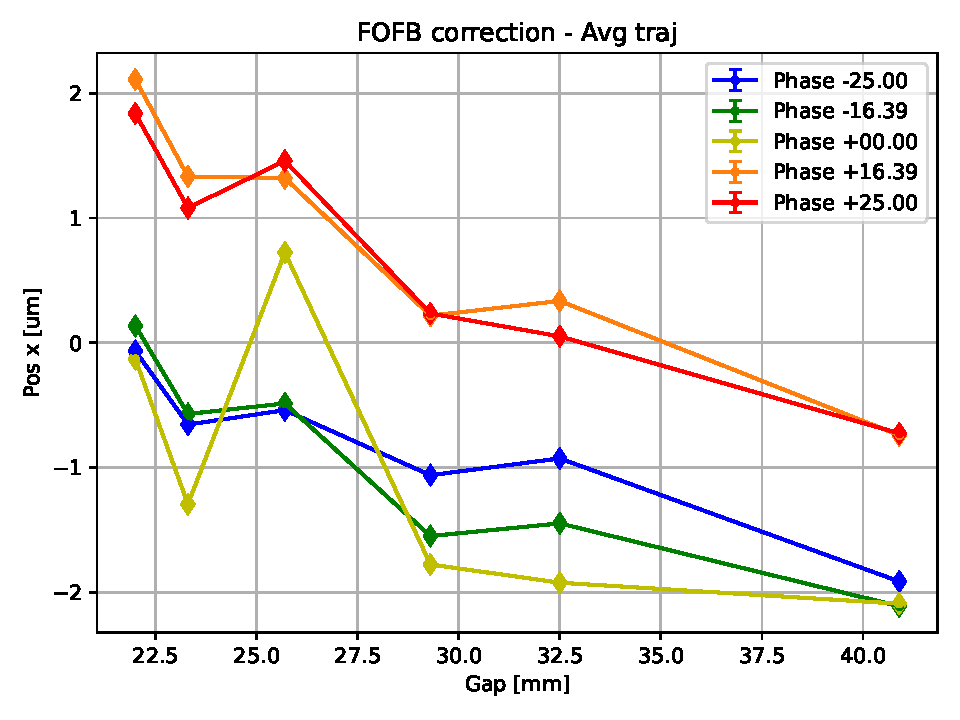
\includegraphics[width=0.9\linewidth, height=7cm]{figs/FOFB-avg-trajx.pdf} 
\label{fig:subimfofbtx}
\end{subfigure}
\begin{subfigure}{0.5\textwidth}
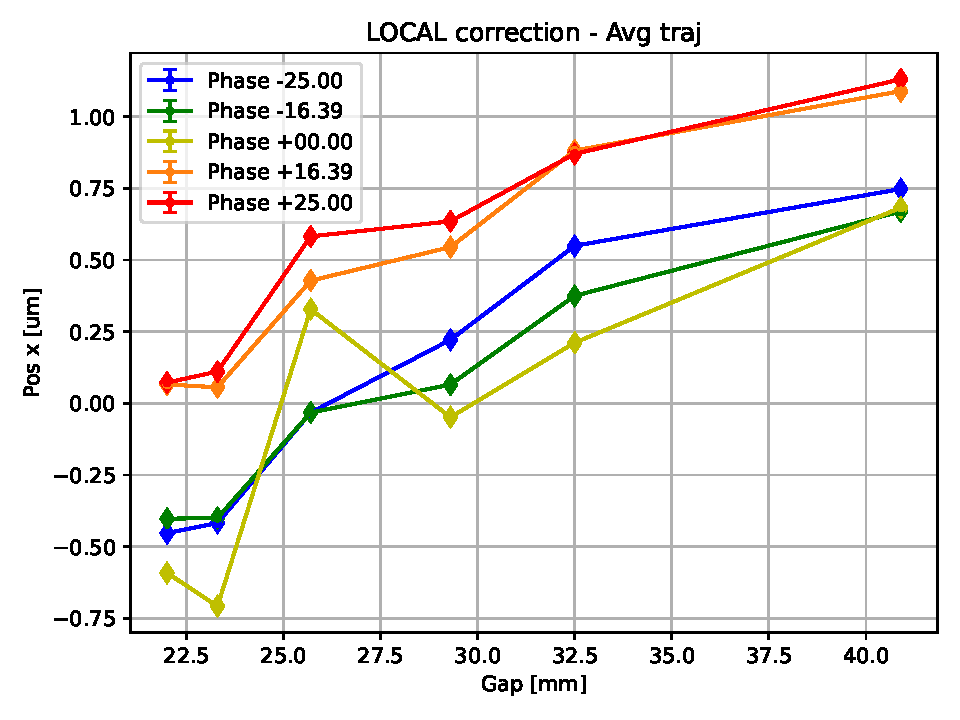
\includegraphics[width=0.9\linewidth, height=7cm]{figs/LOCAL-avg-trajx.pdf}
\label{fig:subimlocaltx}
\end{subfigure}
\caption{Deslocamento horizontal médio no ID após correções}
\label{fig:trajx}
\end{figure}

Os gráficos da figura \ref{fig:trajy} mostram agora o deslocamento vertical médio para cada método de correção. As barras verticais representam o desvio padrão do deslocamento.

\begin{figure}[H]
\begin{subfigure}{0.5\textwidth}
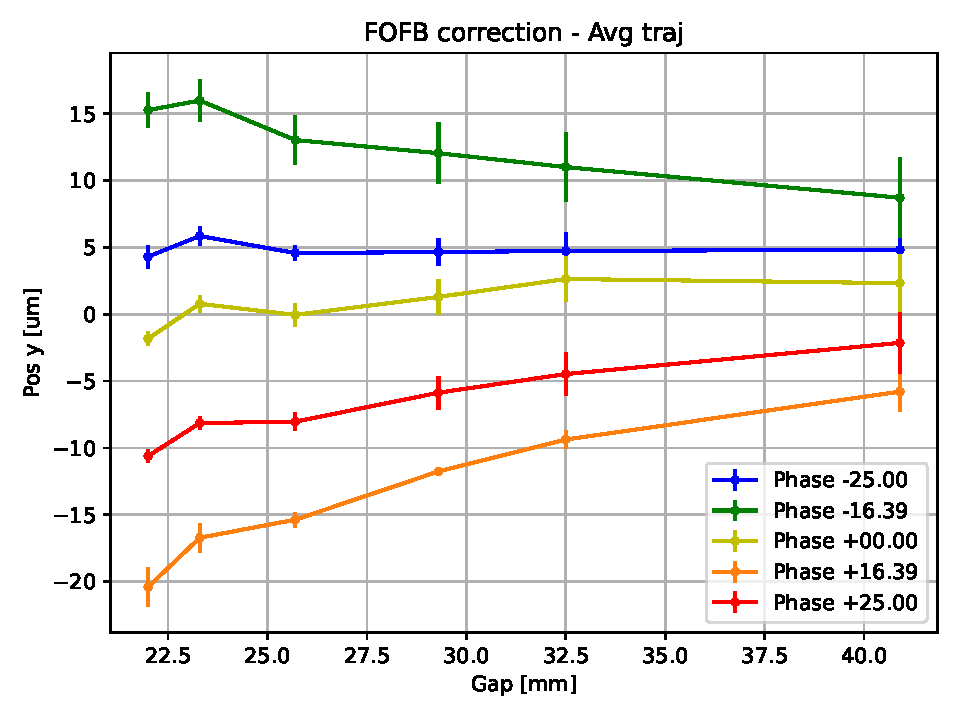
\includegraphics[width=0.9\linewidth, height=7cm]{figs/FOFB-avg-trajy.pdf} 
\label{fig:subimfofbty}
\end{subfigure}
\begin{subfigure}{0.5\textwidth}
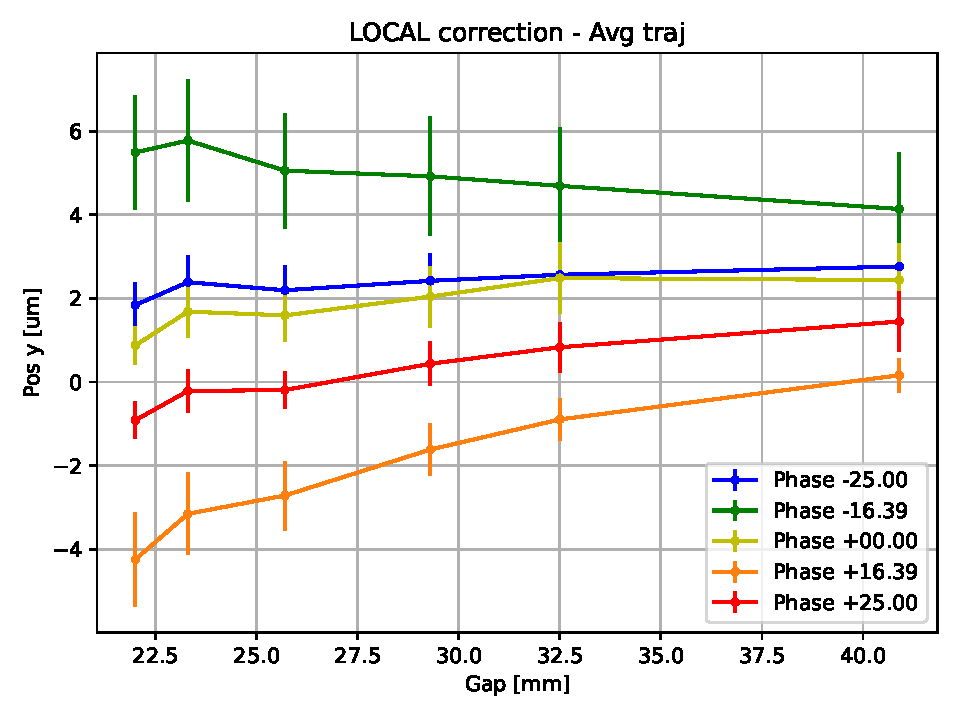
\includegraphics[width=0.9\linewidth, height=7cm]{figs/LOCAL-avg-trajy.pdf}
\label{fig:subimlocalty}
\end{subfigure}
\caption{Deslocamento horizontal médio no ID após correções}
\label{fig:trajy}
\end{figure}

As figuras \ref{fig:angx} e \ref{fig:angy} exibem os ângulos médios do feixe ao realizar sua passagem pelos campos do ID.

\begin{figure}[H]
\begin{subfigure}{0.5\textwidth}
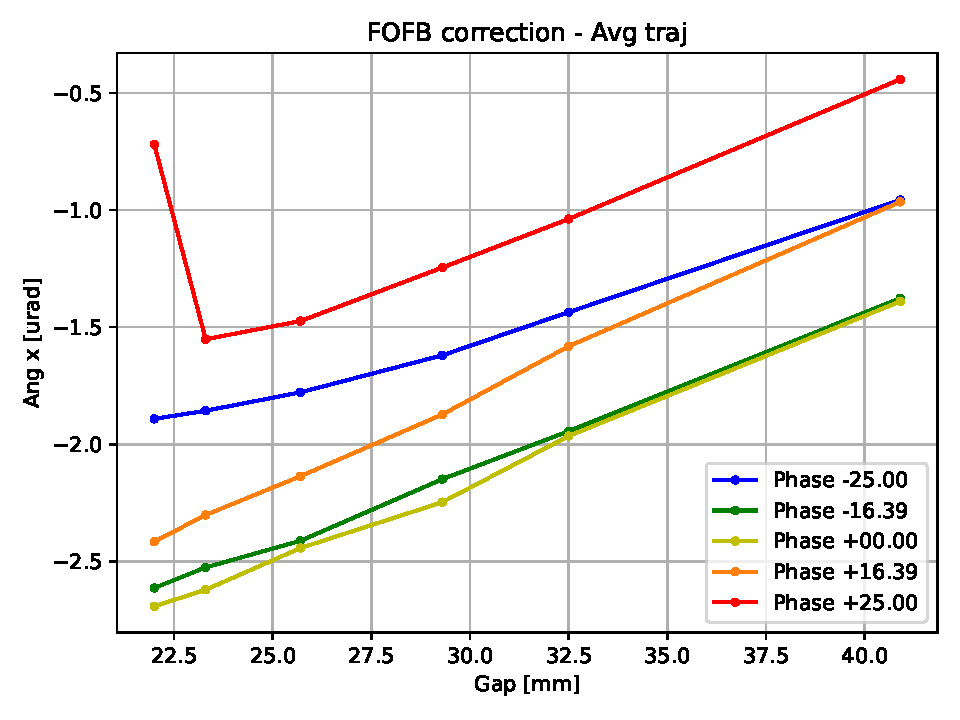
\includegraphics[width=0.9\linewidth, height=7cm]{figs/FOFB-avg-angx.pdf} 
\label{fig:subimfofbangx}
\end{subfigure}
\begin{subfigure}{0.5\textwidth}
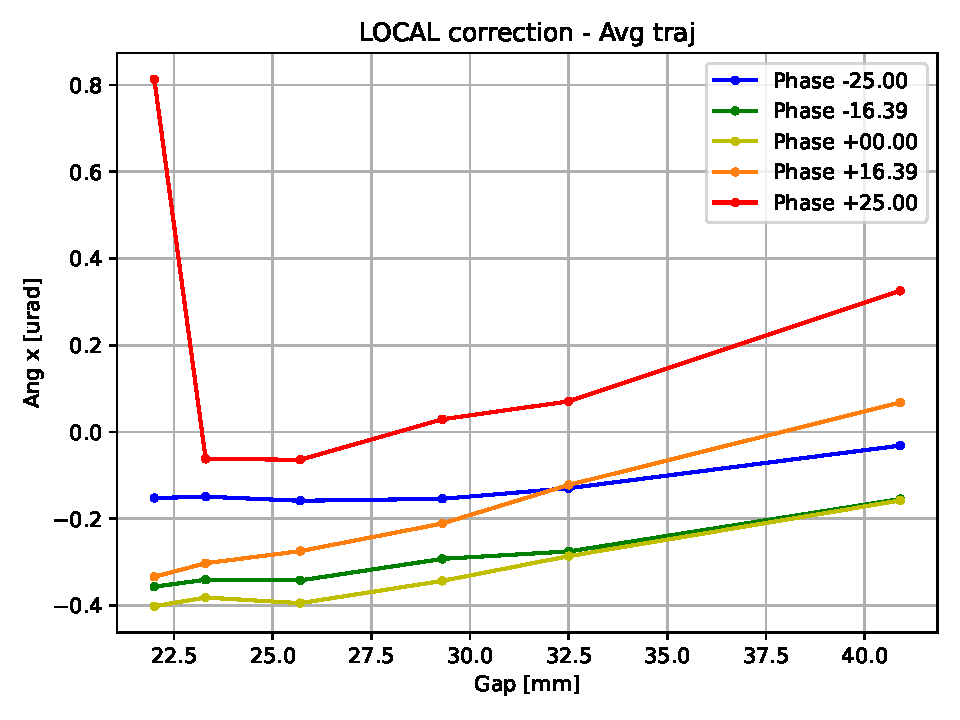
\includegraphics[width=0.9\linewidth, height=7cm]{figs/LOCAL-avg-angx.pdf}
\label{fig:subimlocalangx}
\end{subfigure}
\caption{Ângulo horizontal médio no ID após correções}
\label{fig:angx}
\end{figure}

\begin{figure}[H]
\begin{subfigure}{0.5\textwidth}
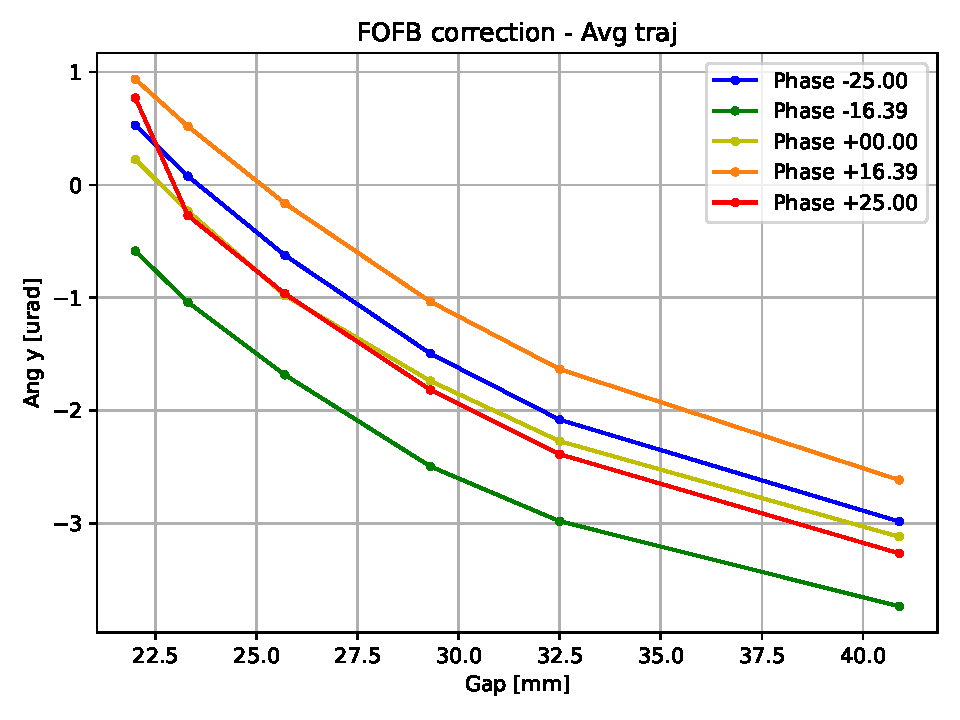
\includegraphics[width=0.9\linewidth, height=7cm]{figs/FOFB-avg-angy.pdf} 
\label{fig:subimfofbangy}
\end{subfigure}
\begin{subfigure}{0.5\textwidth}
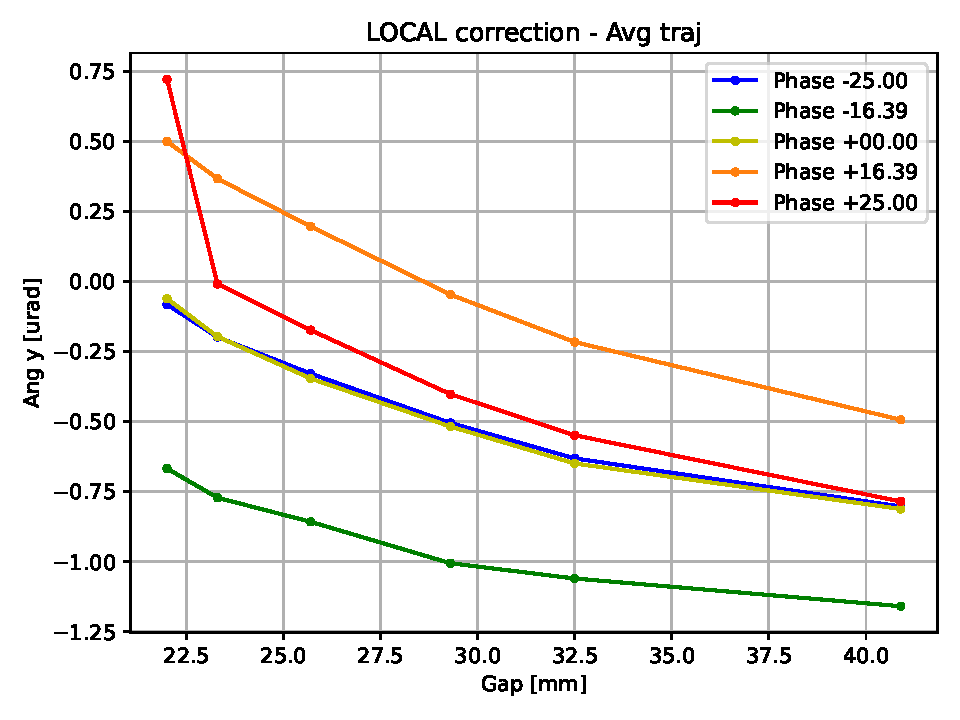
\includegraphics[width=0.9\linewidth, height=7cm]{figs/LOCAL-avg-angy.pdf}
\label{fig:subimlocalangy}
\end{subfigure}
\caption{Ângulo vertical médio no ID após correções}
\label{fig:angy}
\end{figure}

As figuras a seguir exibem uma comparação entre os kicks das corretoras locais e os kicks das corretoras do FOFB mais próximas do ID

\begin{figure}[H]
\begin{subfigure}{0.5\textwidth}
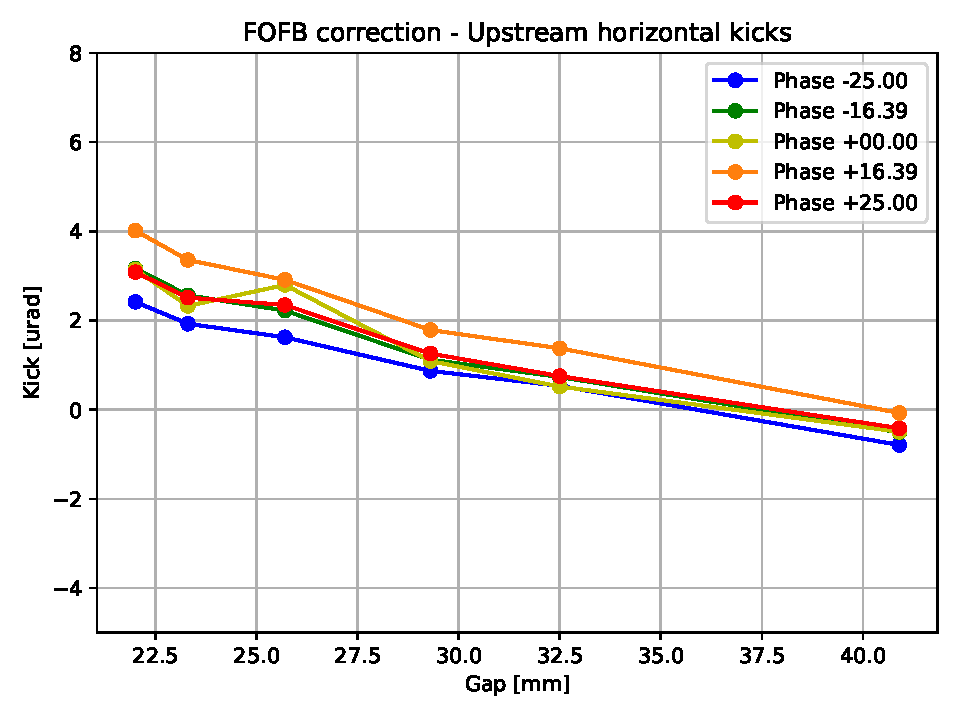
\includegraphics[width=0.9\linewidth, height=7cm]{figs/FOFB-up-kickx.pdf} 
\label{fig:subimfofbup}
\end{subfigure}
\begin{subfigure}{0.5\textwidth}
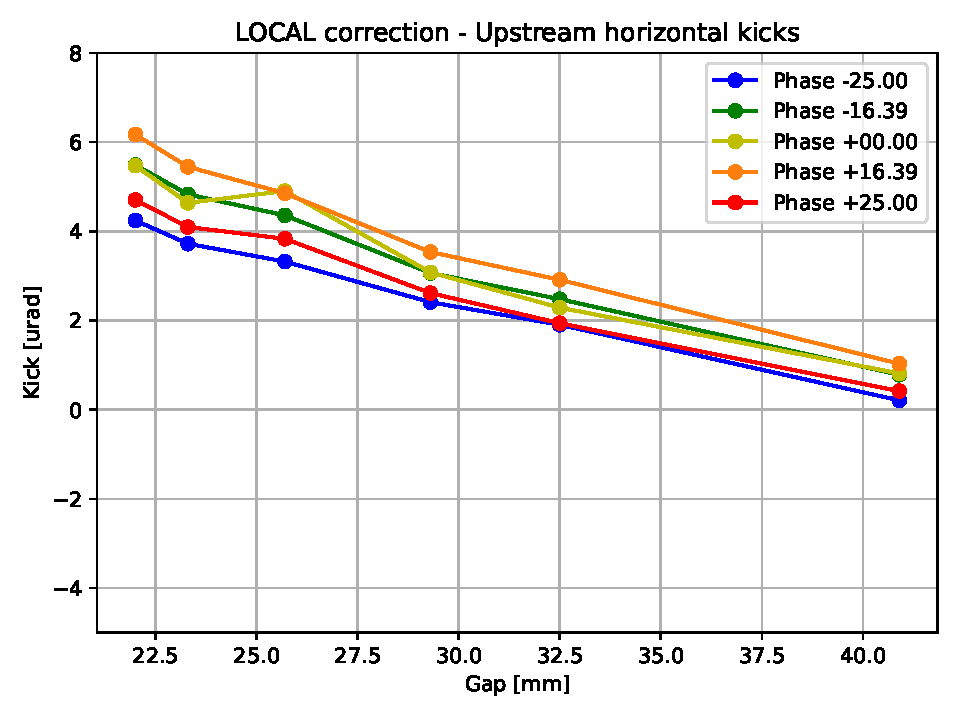
\includegraphics[width=0.9\linewidth, height=7cm]{figs/LOCAL-up-kickx.pdf}
\label{fig:subimlocalup}
\end{subfigure}
\caption{Kicks horizontais nas corretoras upstream do FOFB (esquerda) e locais (direita)}
\label{fig:upx}
\end{figure}

\begin{figure}[H]
\begin{subfigure}{0.5\textwidth}
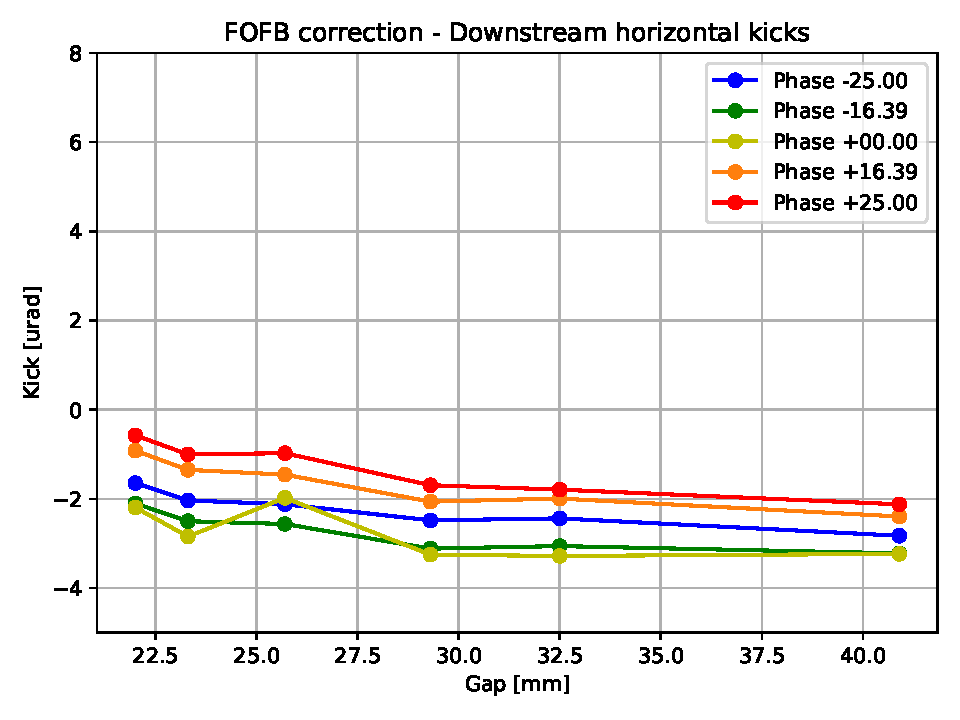
\includegraphics[width=0.9\linewidth, height=7cm]{figs/FOFB-down-kickx.pdf} 
\label{fig:subimfofbdown}
\end{subfigure}
\begin{subfigure}{0.5\textwidth}
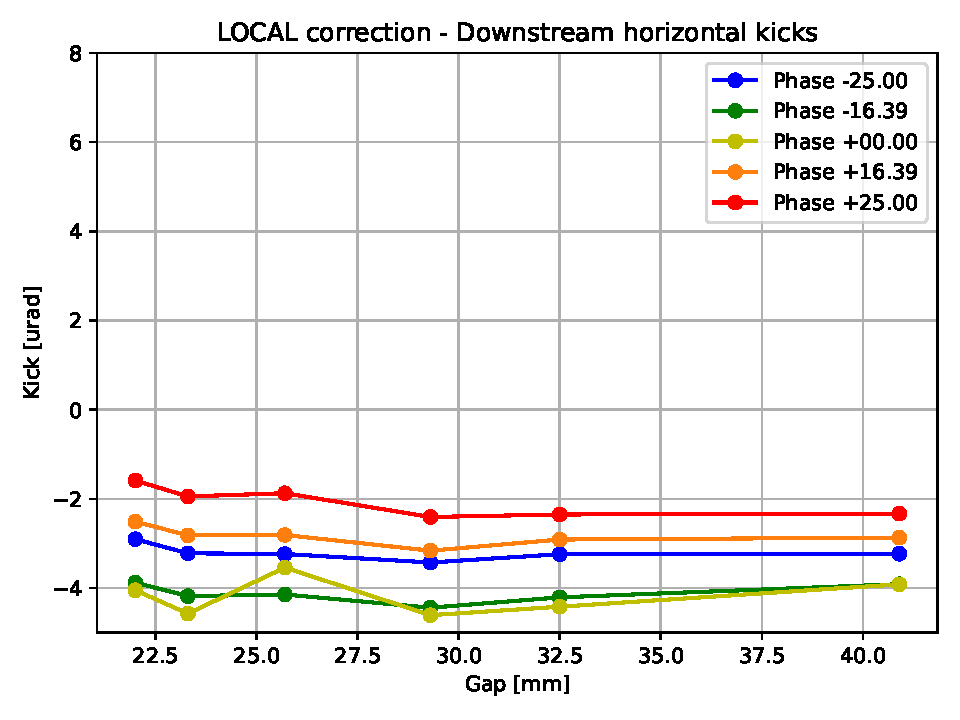
\includegraphics[width=0.9\linewidth, height=7cm]{figs/LOCAL-down-kickx.pdf}
\label{fig:subimlocaldown}
\end{subfigure}
\caption{Kicks horizontais nas corretoras downstream do FOFB (esquerda) e locais (direita)}
\label{fig:downx}
\end{figure}

\begin{figure}[H]
\begin{subfigure}{0.5\textwidth}
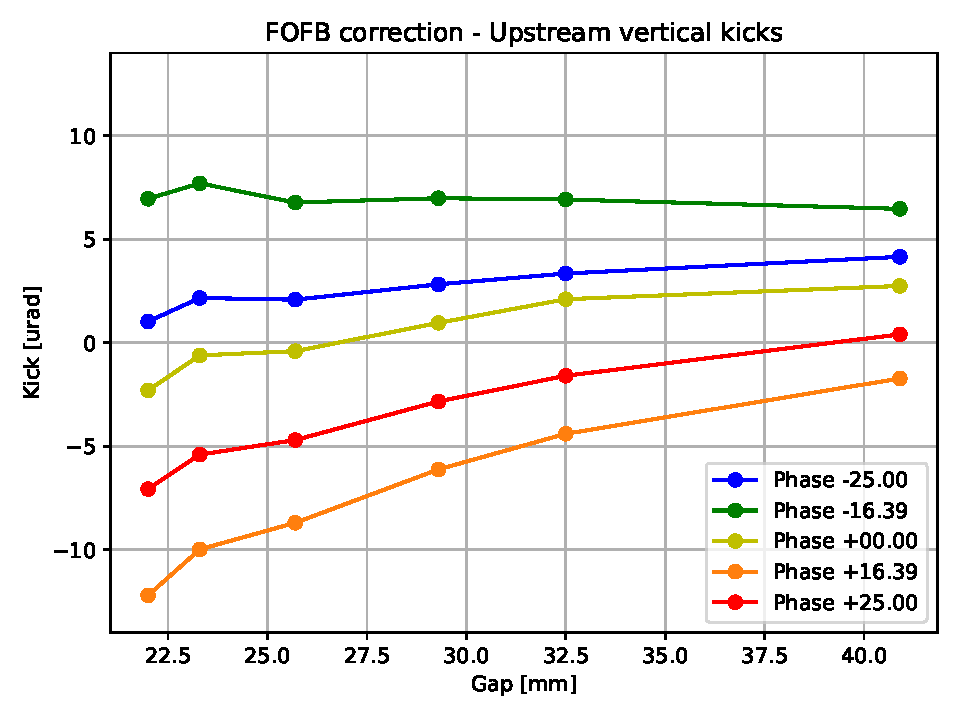
\includegraphics[width=0.9\linewidth, height=7cm]{figs/FOFB-up-kicky.pdf} 
\label{fig:subimfofbupy}
\end{subfigure}
\begin{subfigure}{0.5\textwidth}
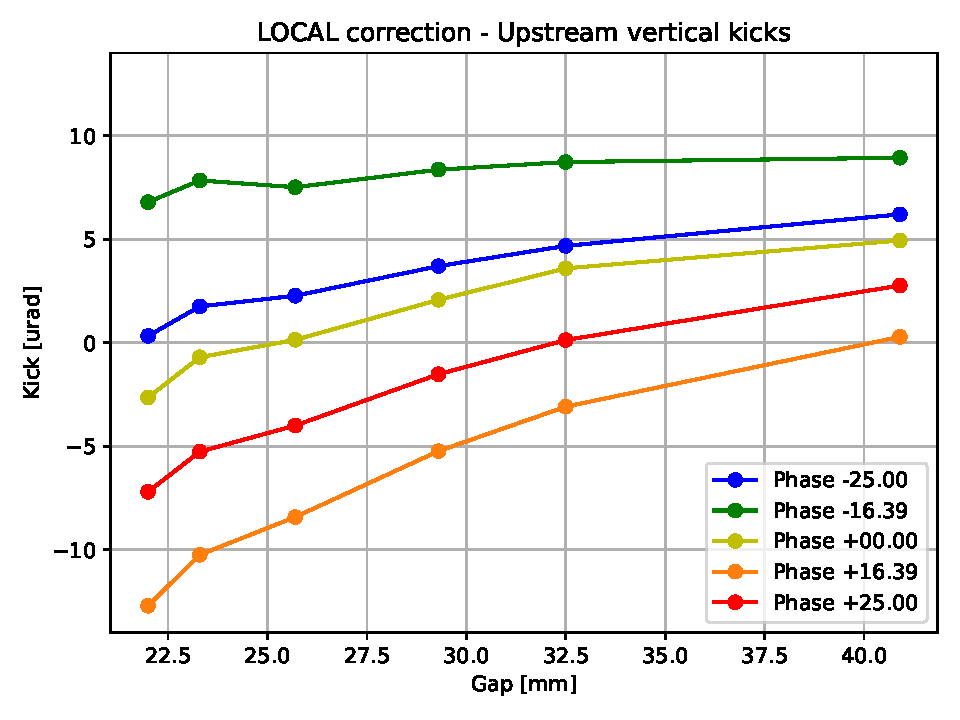
\includegraphics[width=0.9\linewidth, height=7cm]{figs/LOCAL-up-kicky.pdf}
\label{fig:subimlocalupy}
\end{subfigure}
\caption{Kicks verticais nas corretoras upstream do FOFB (esquerda) e locais (direita)}
\label{fig:upy}
\end{figure}

\begin{figure}[H]
\begin{subfigure}{0.5\textwidth}
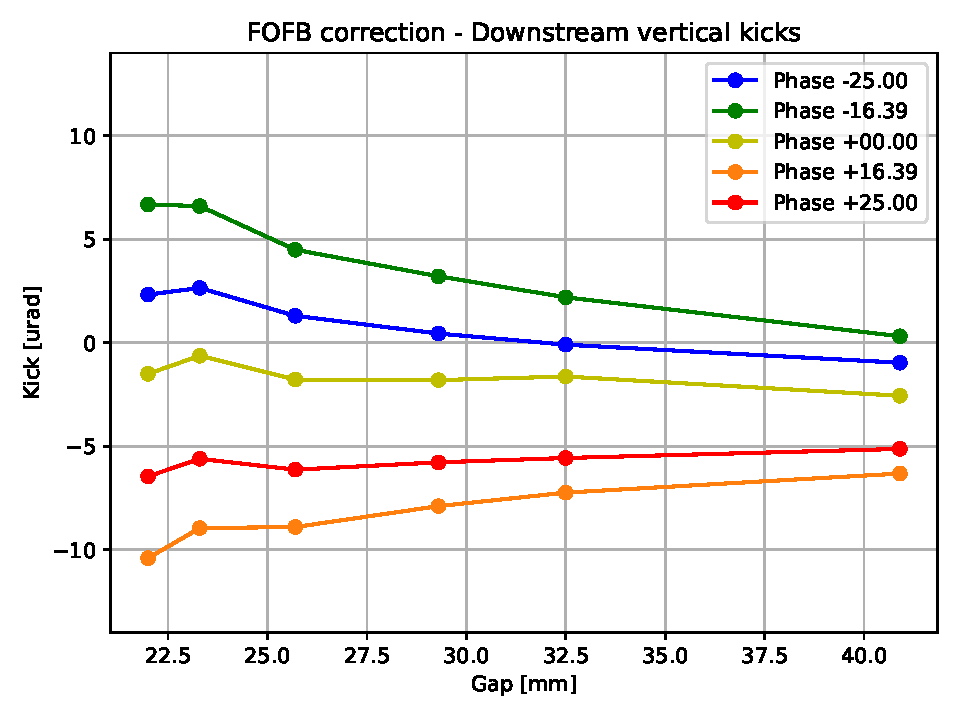
\includegraphics[width=0.9\linewidth, height=7cm]{figs/FOFB-down-kicky.pdf} 
\label{fig:subimfofbdowny}
\end{subfigure}
\begin{subfigure}{0.5\textwidth}
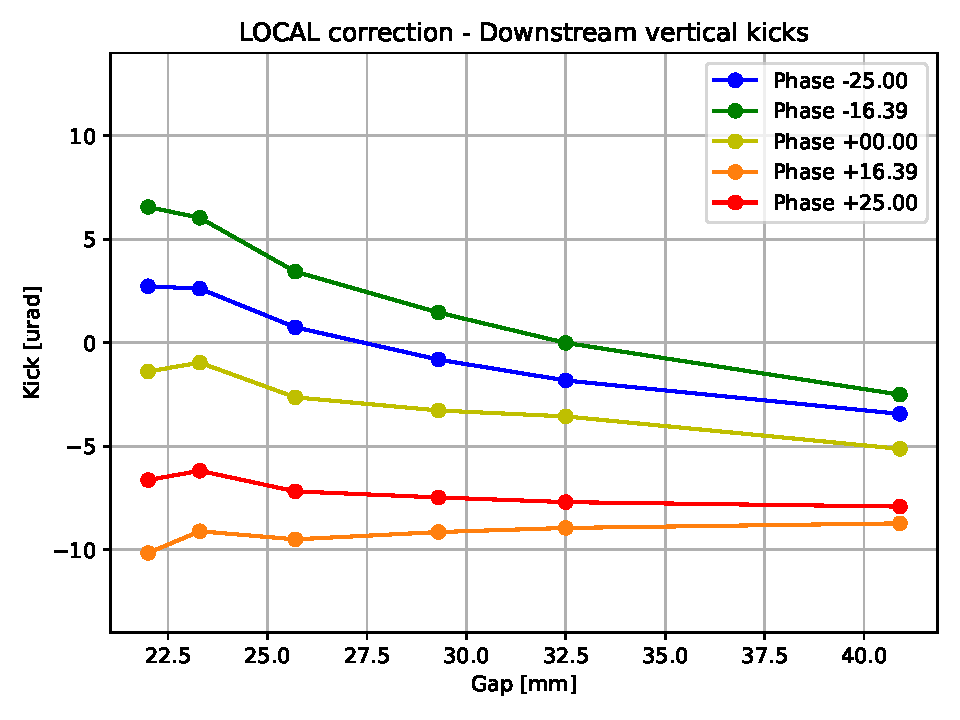
\includegraphics[width=0.9\linewidth, height=7cm]{figs/LOCAL-down-kicky.pdf}
\label{fig:subimlocaldowny}
\end{subfigure}
\caption{Kicks verticais nas corretoras downstream do FOFB (esquerda) e locais (direita)}
\label{fig:downy}
\end{figure}


\subsection{Fase 00.00 mm}

\subsubsection{Campo vs gap}
A figura abaixo exibe a dependência do campo efetivo com o gap, na legenda dos gráficos se encontra a função usada para a realização do "fitting" dos dados, vale ressaltar que esse é o campo ao longo da trajetória dos elétrons, que é muito próximo do campo nominal no eixo central. Abaixo da figura encontra-se a tabela 1,que contém alguns pontos das curvas da figura e pode ser útil durante o comissionamento.
\begin{figure}[H]
\hspace{4cm}
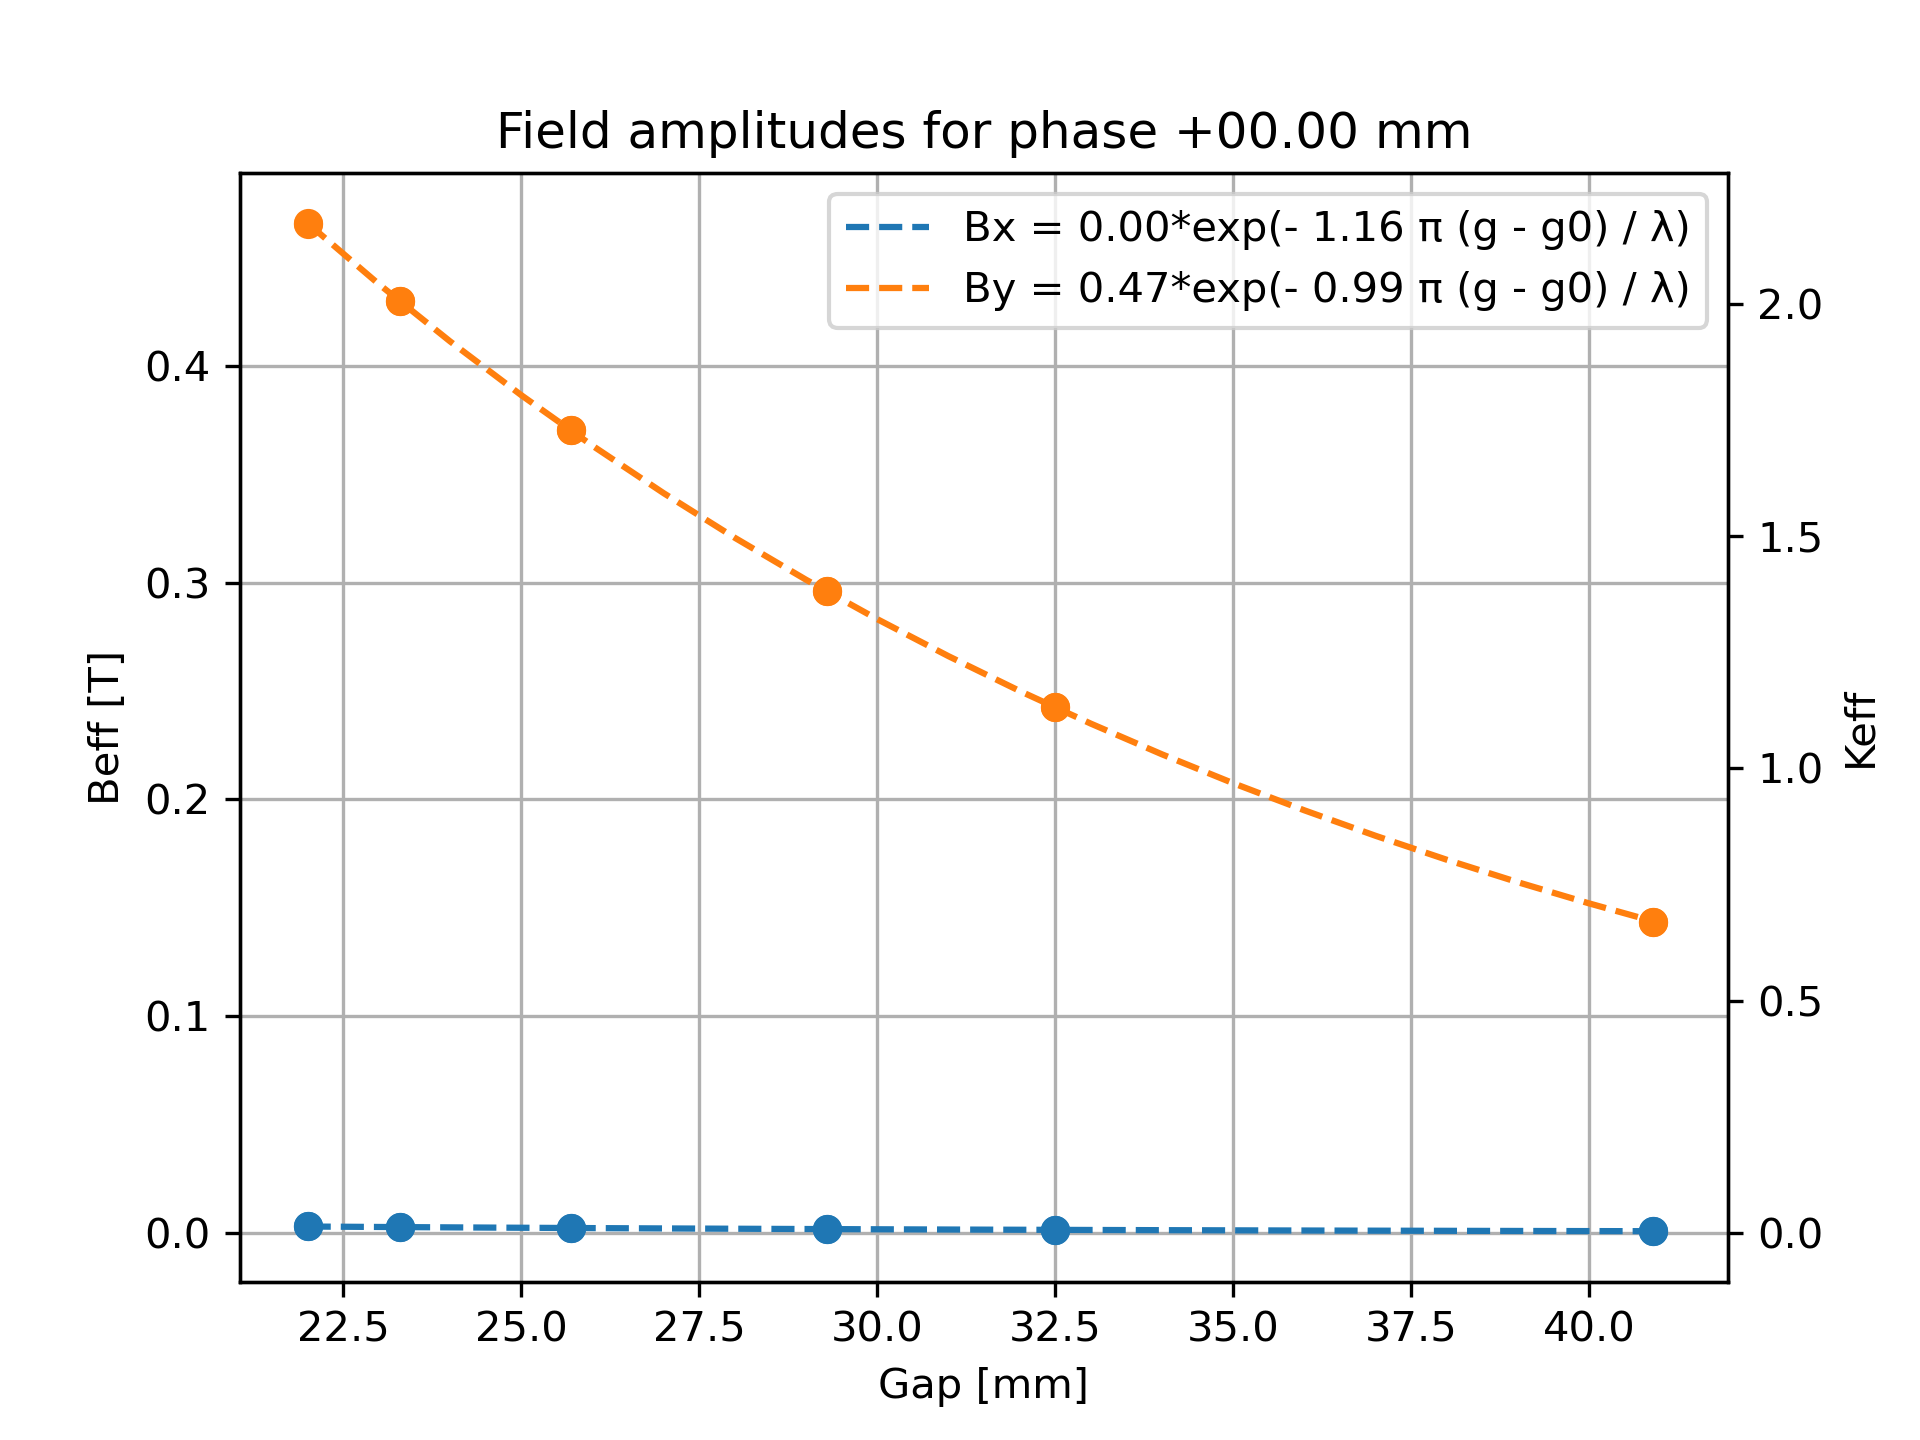
\includegraphics[width=0.5\textwidth]{figs/phase0 B vs gap.png}
\caption{Beff vs gap fase = 00.00 mm}
\label{fig:fieldgap0}
\end{figure}

\begin{table}[H]
\caption{Beff vs gap fase = 00.00 mm}
\centering
\begin{tabular}{|c|c|}
\hline
   Gap [mm] &   By [T] \\
\hline
       22.0 &             0.47 \\
       23.3 &             0.43 \\
       25.7 &             0.37 \\
       29.3 &             0.30  \\
       32.5 &             0.24 \\
       40.9 &             0.14 \\
\hline
\end{tabular}
\end{table}

\paragraph{} As figuras abaixo exibem os campos normalizados do ID na configuração em questão.

\begin{figure}[H]
\begin{center}
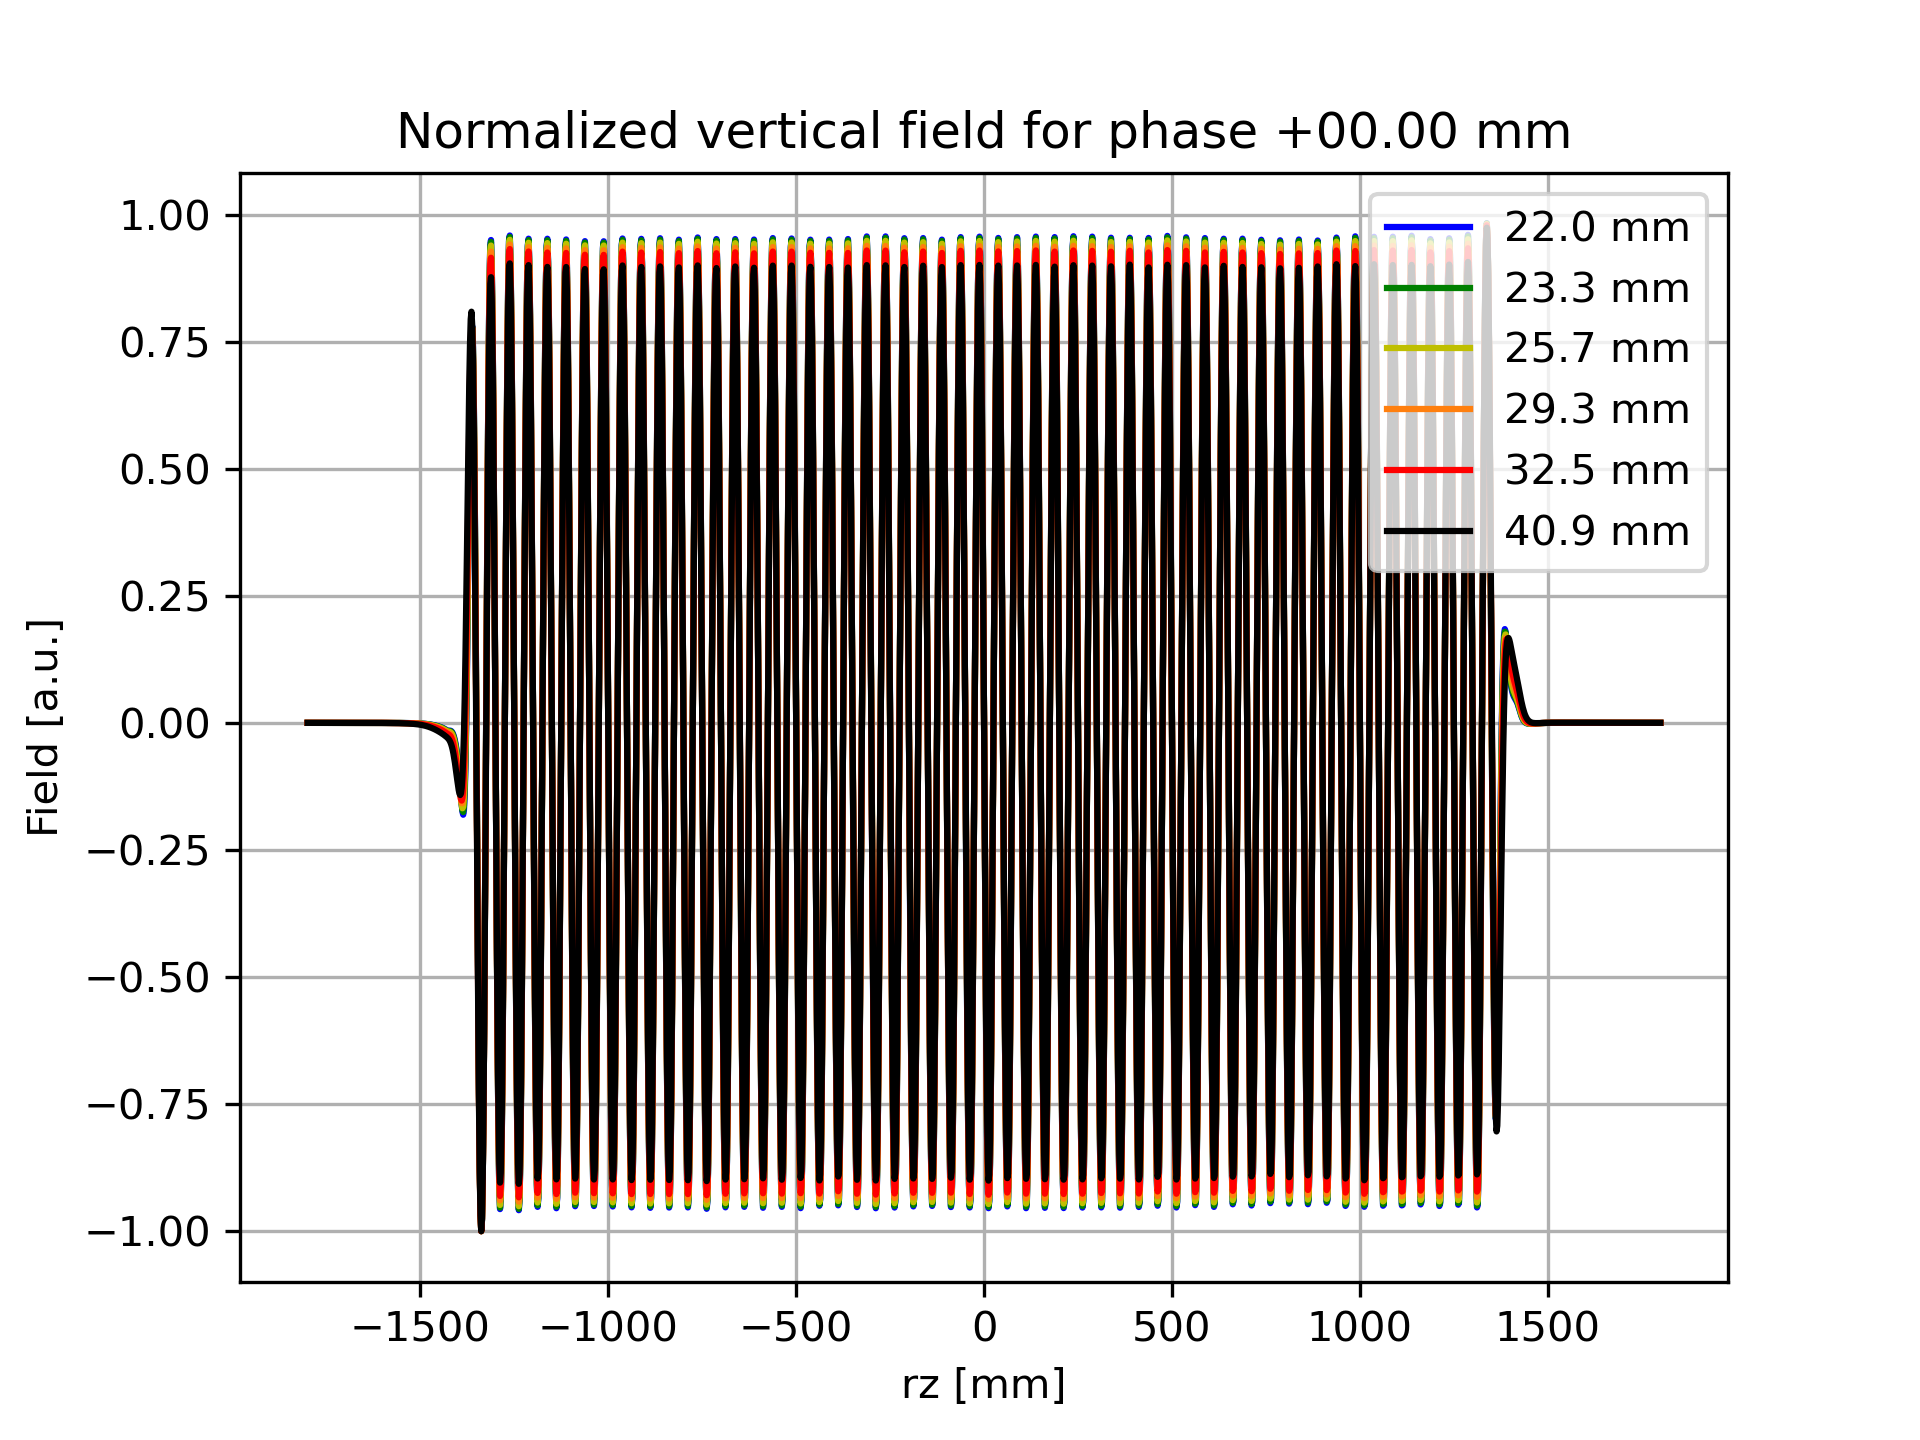
\includegraphics[width=0.5\textwidth]{figs/phase0 By.png}
\caption{Componente vertical de campo normalizada}
\label{fig:by0}
\end{center}
\end{figure}

\begin{figure}[H]
\begin{subfigure}{0.5\textwidth}
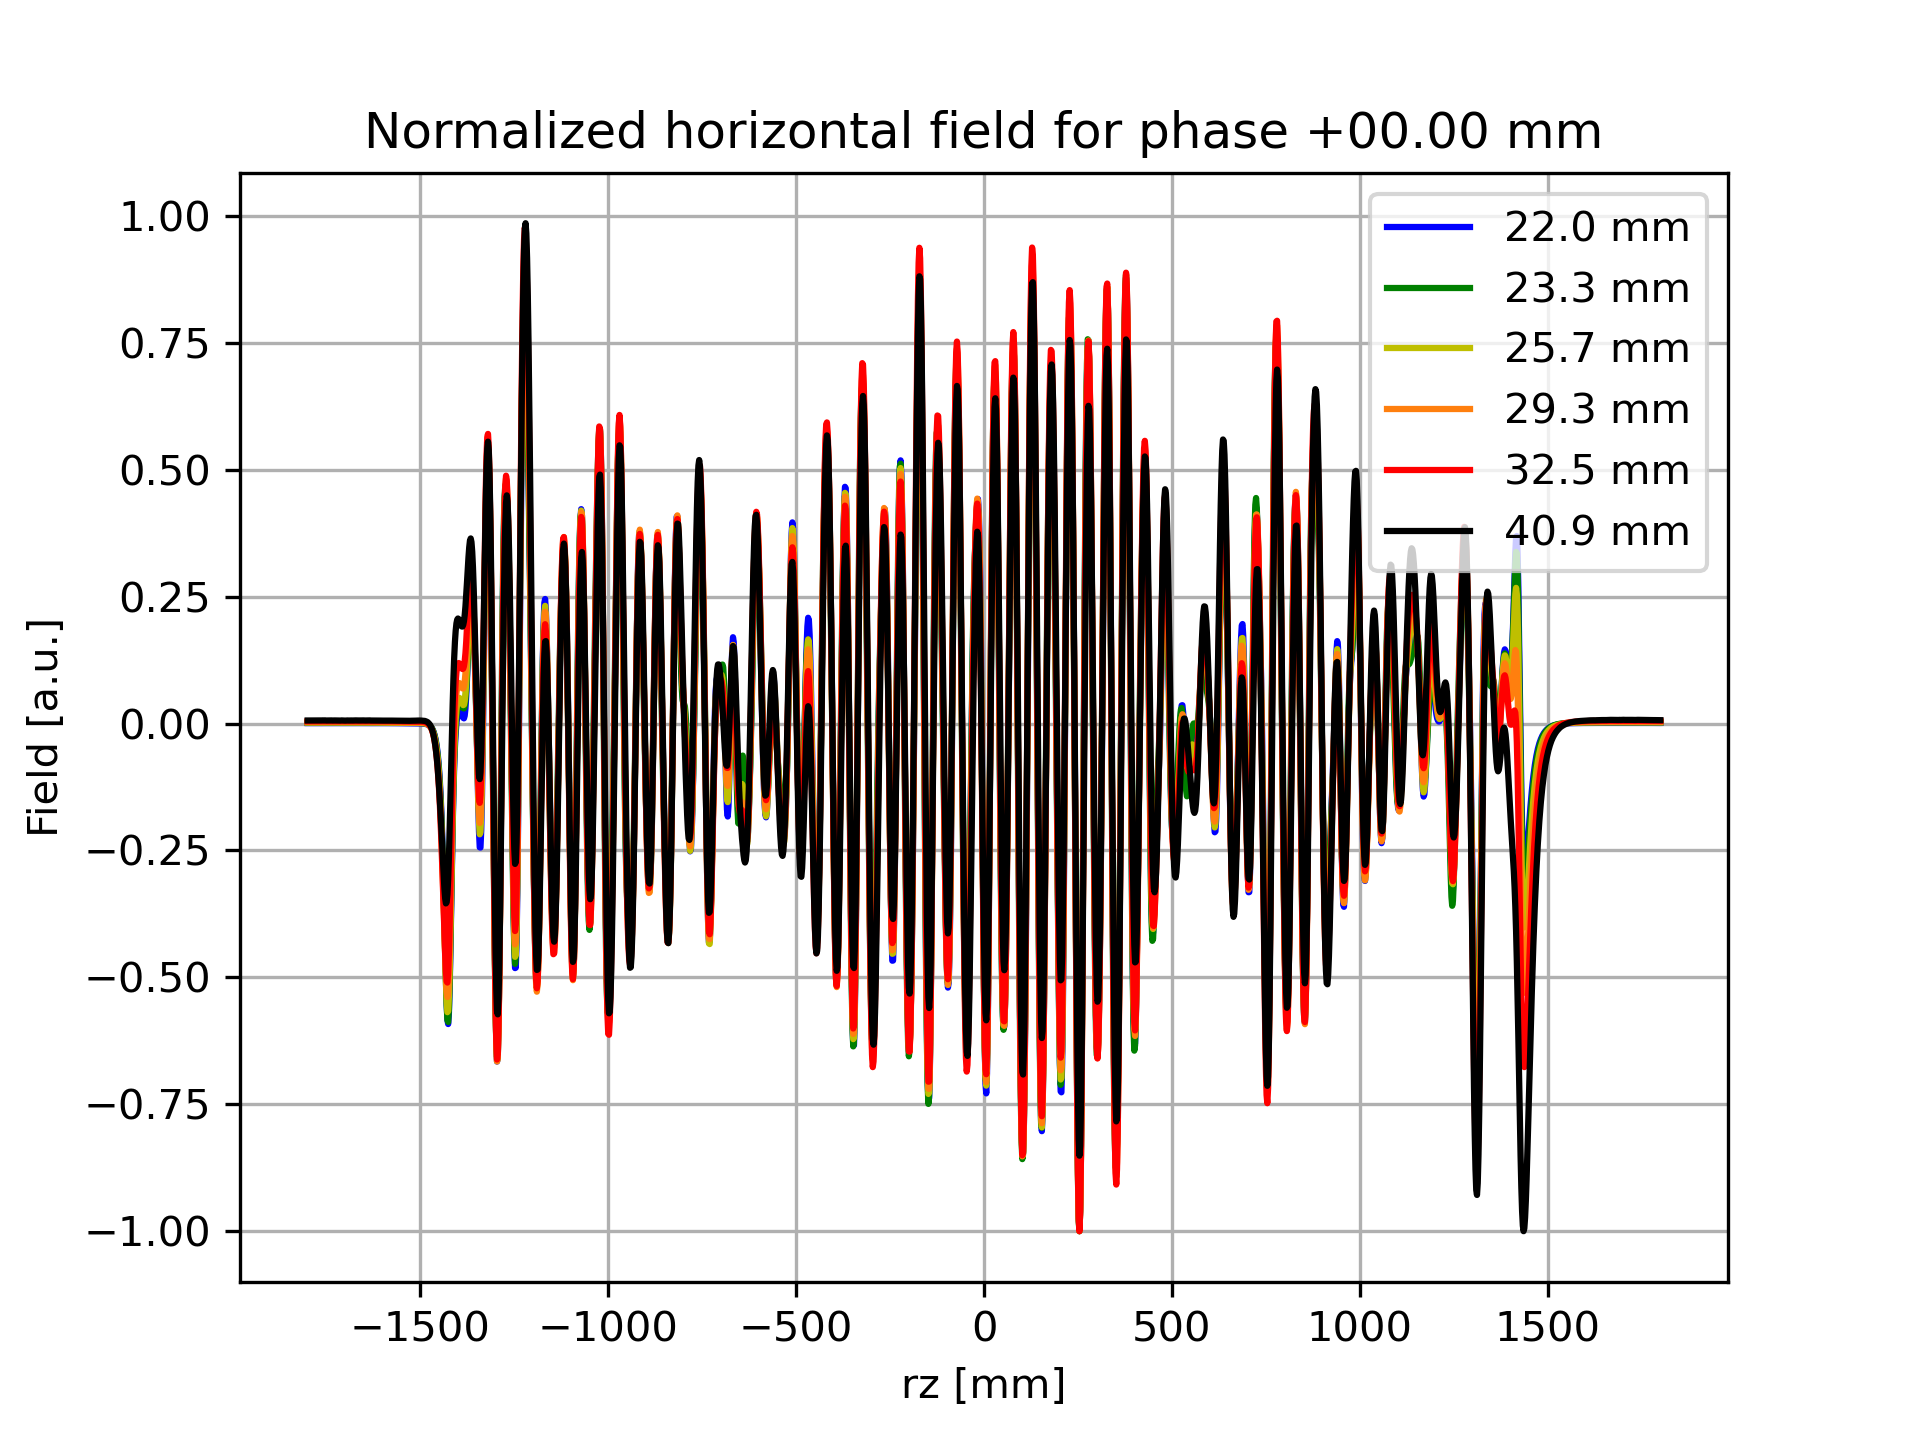
\includegraphics[width=0.9\linewidth, height=7cm]{figs/phase0 Bx.png} 
\label{fig:subim1}
\end{subfigure}
\begin{subfigure}{0.5\textwidth}
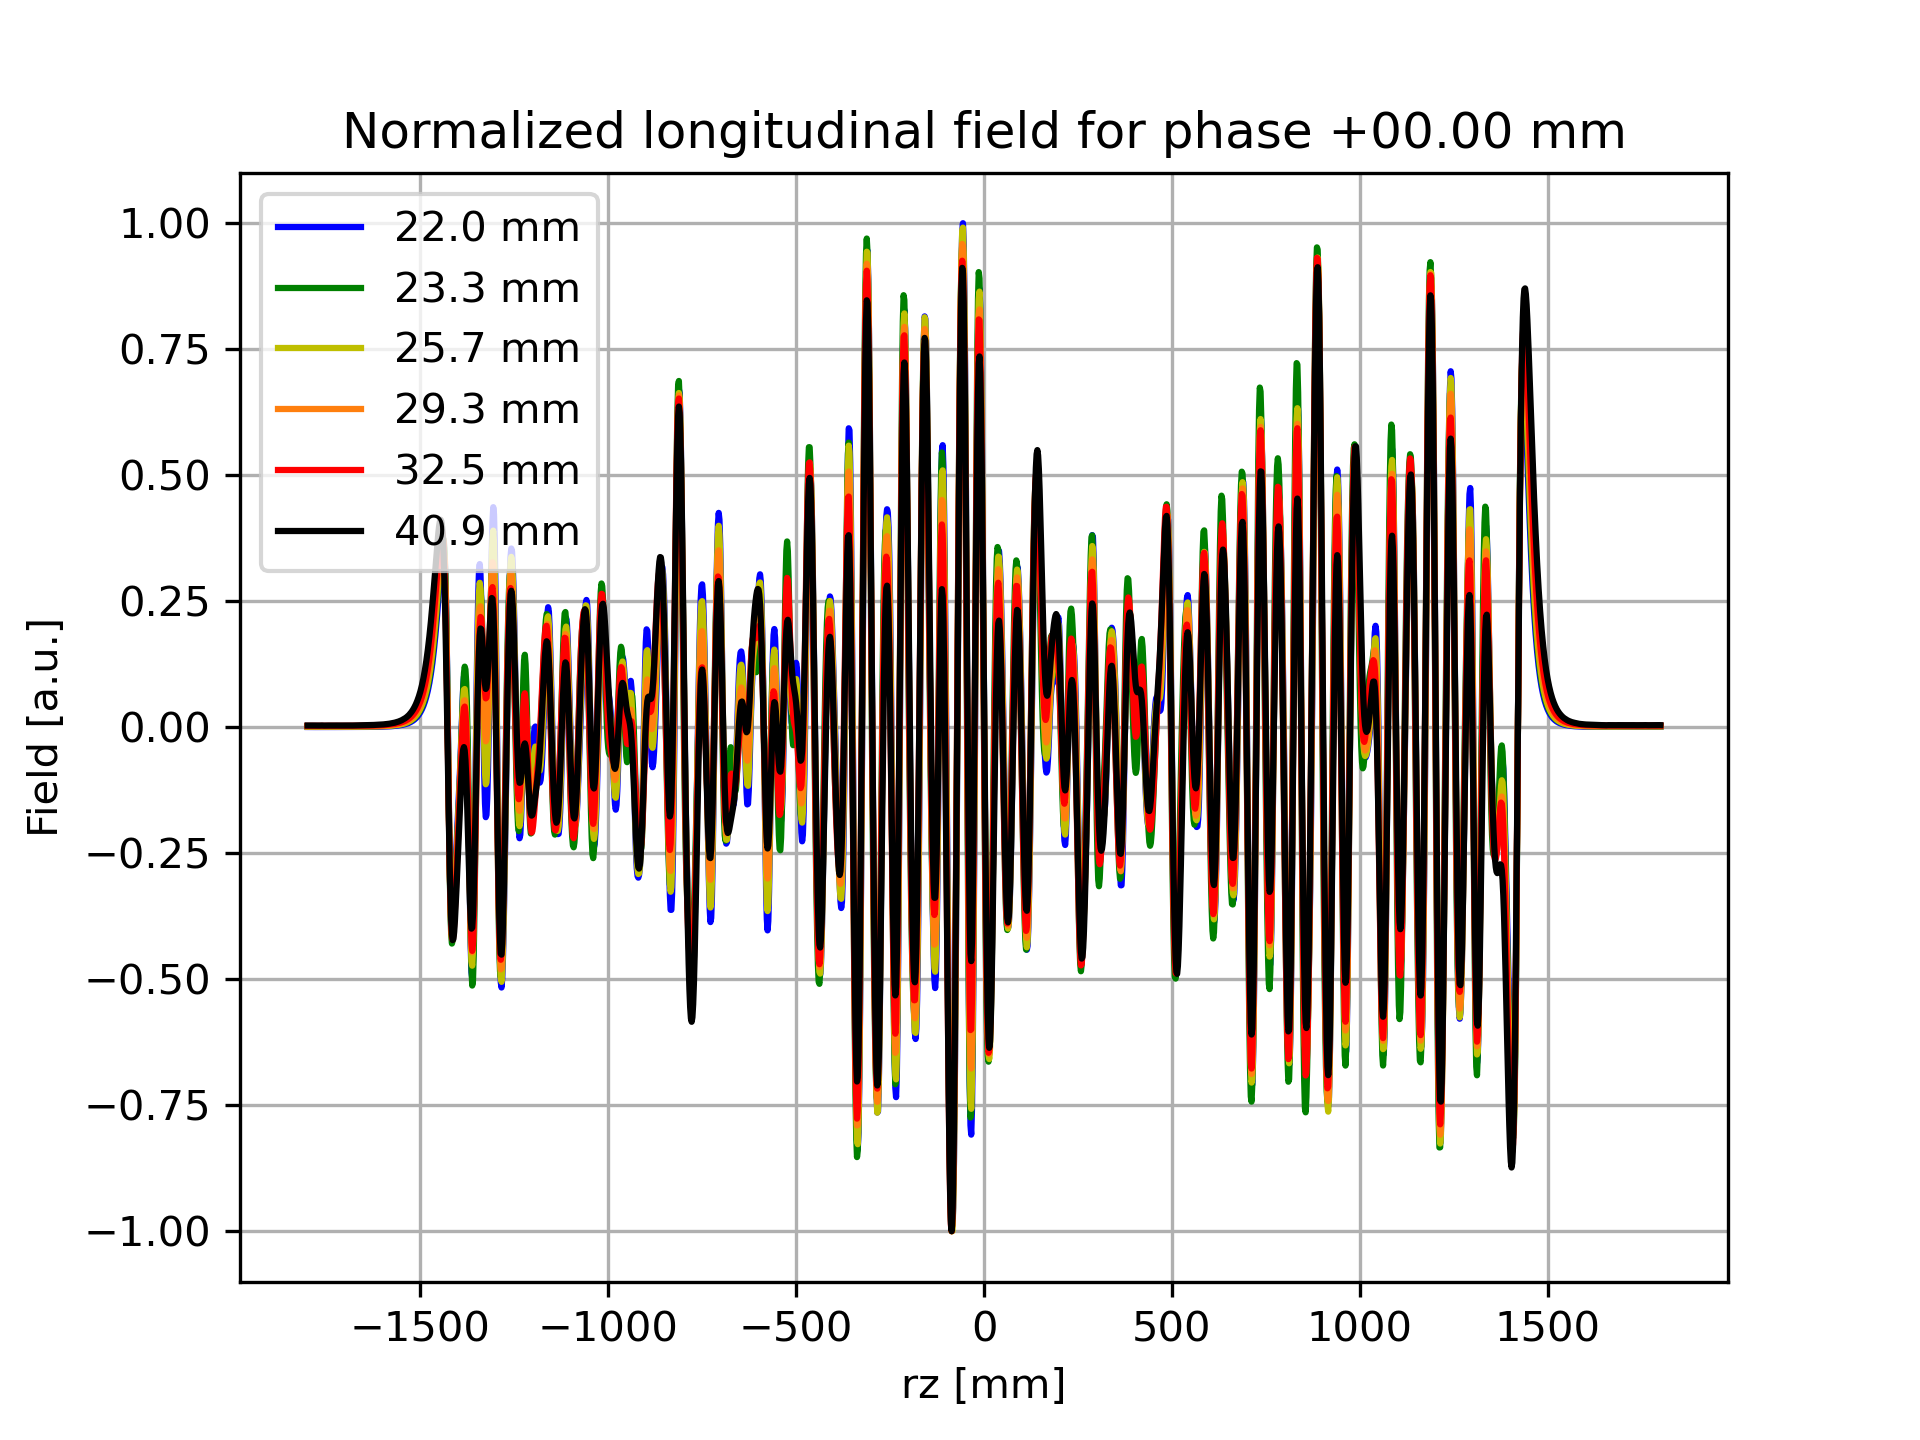
\includegraphics[width=0.9\linewidth, height=7cm]{figs/phase0 Bz.png}
\label{fig:subim2}
\end{subfigure}
\caption{Componentes de campo horizontais (esquerda) e longitudinal (direita)}
\label{fig:bx_bz0}
\end{figure}

\subsubsection{Correções de órbita}

A tabela \ref{tab:corff0} exibe os kicks necessários nas corretoras locais para que a distorção de órbita gerada pelo ID seja corrigida (tabela de feedforward). A linha referente ao gap 36 da tabela foi obtida por meio de medidas com o feixe, durante o comissionamento do ID.

\begin{table}[H]
\centering
\caption{Tabela de correção local}
\begin{tabular}{|c|c|c|c|c|}
\hline
Gap {[}mm{]} & $\Delta$px up {[}$\mu$rad{]} & $\Delta$px down {[}$\mu$rad{]} & $\Delta$py up {[}$\mu$rad{]} & $\Delta$py down {[}$\mu$rad{]} \\ \hline
22.0 & 5.81  & -3.82 & -2.73 & -1.37 \\ \hline
23.3 & 4.97  & -4.33 & -0.80 & -1.02 \\ \hline
25.7 & 5.15  & -3.35 &  0.14 & -2.73 \\ \hline
29.3 & 3.32  & -4.37 & 2.12 & -3.43 \\ \hline
32.5 &  2.49 & -4.16 & 3.67 & -3.78 \\ \hline
*36.0 & 4.21 & -0.80 & 1.01 & -7.15 \\ \hline
40.9 & 0.94  & -3.60 & 5.11 & -5.38  \\ \hline
\end{tabular}
\label{tab:corff0}
\end{table}

Os gráficos das figuras \ref{fig:corrx} e \ref{fig:corry} exibem a trajetória média após a correção com FOFB (gráficos da esquerda) e correções locais (gráficos da direita).

\begin{figure}[H]
\begin{subfigure}{0.5\textwidth}
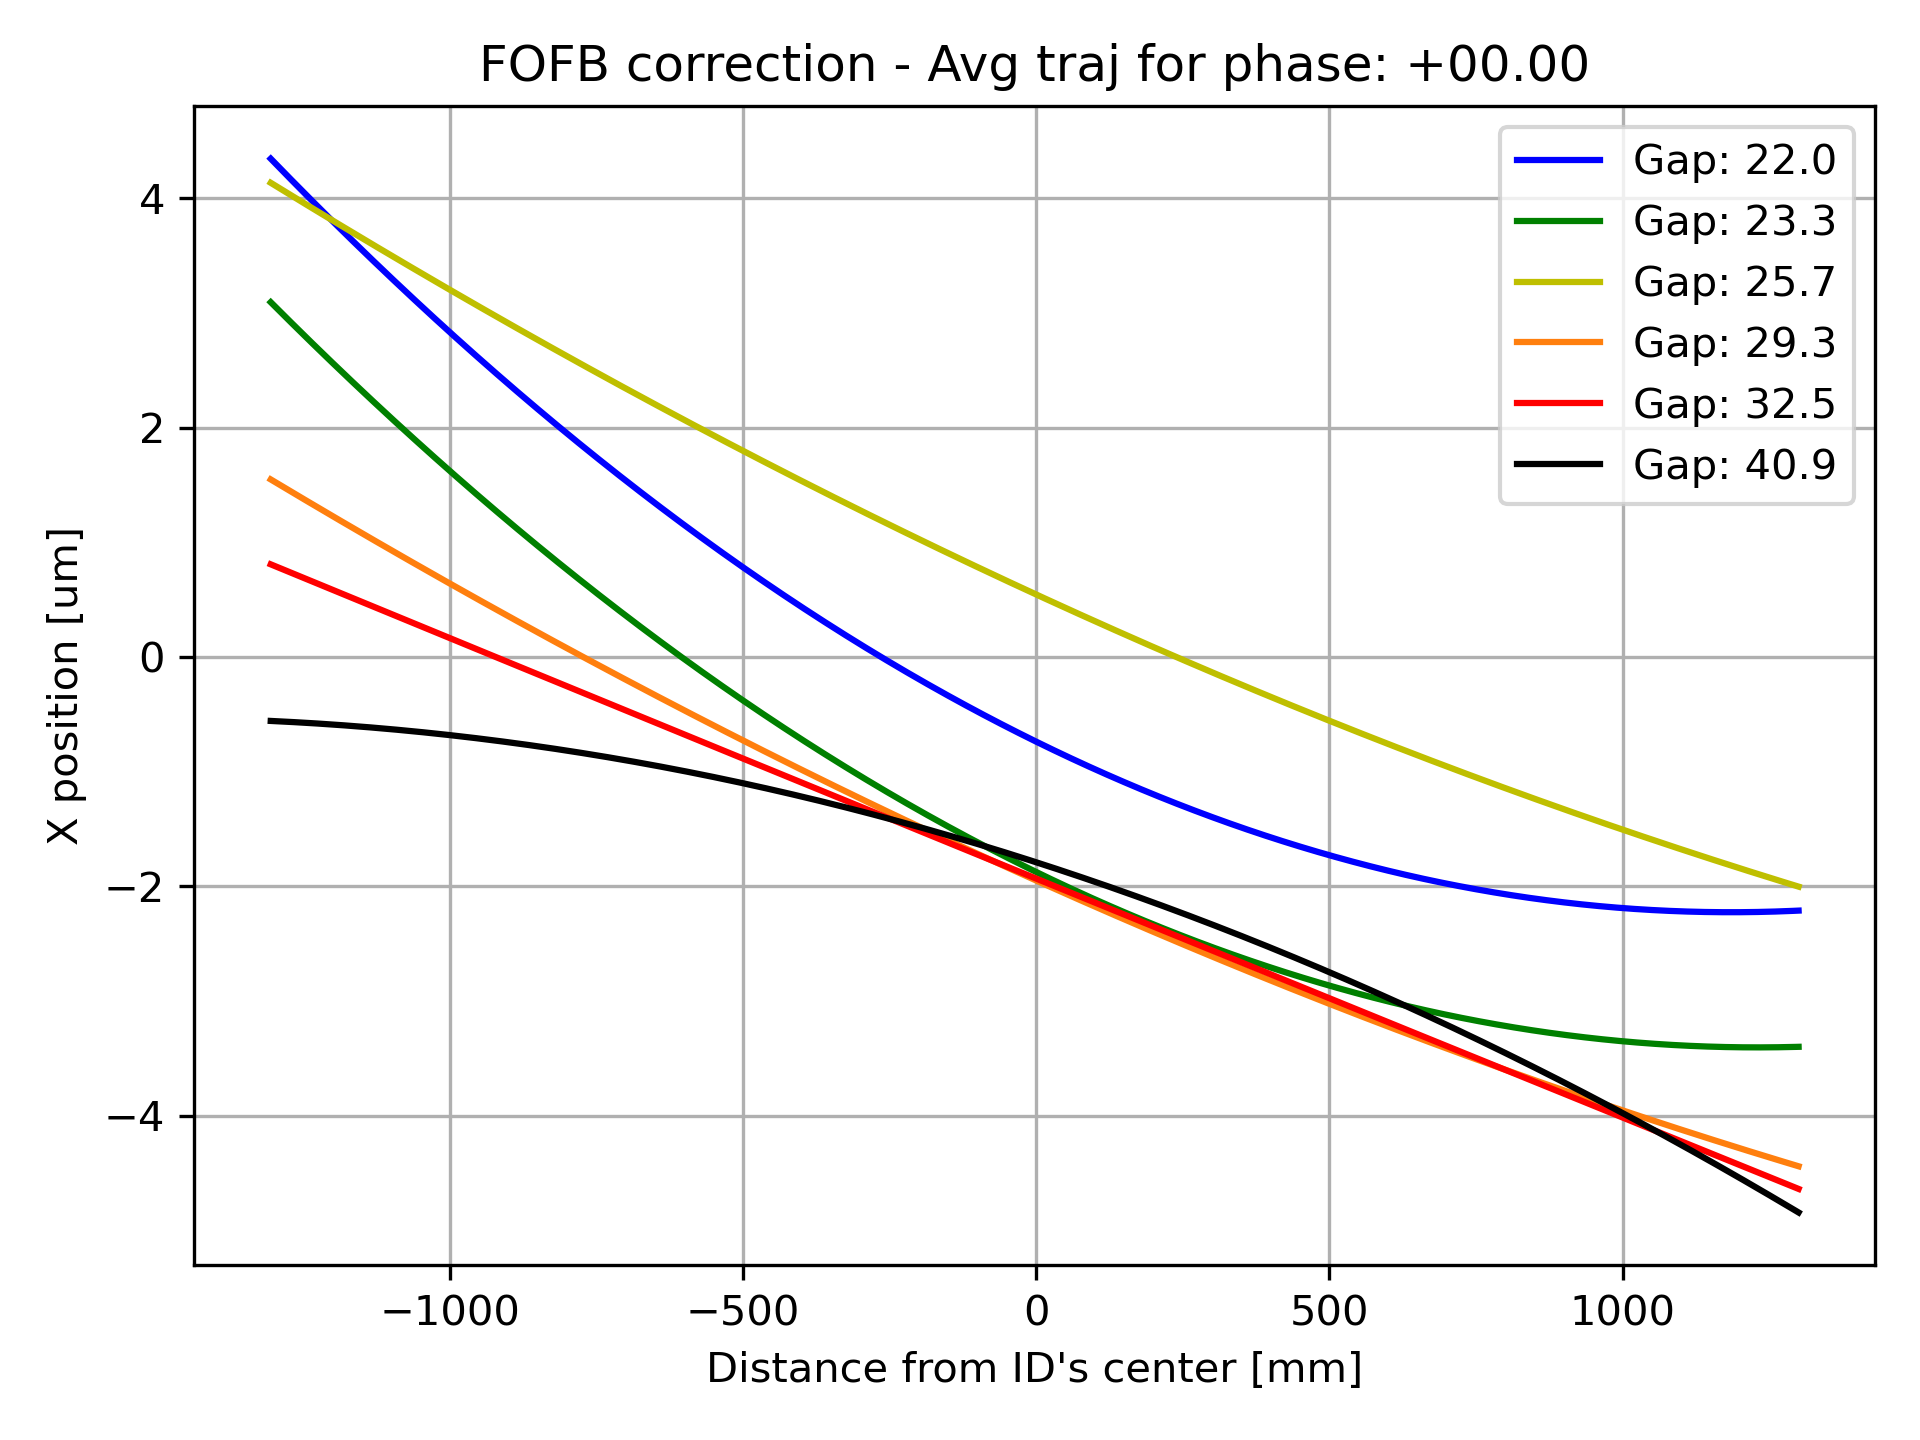
\includegraphics[width=0.9\linewidth, height=7cm]{figs/phase0 horizontal-avg-traj-FOFB.png} 
\label{fig:subim10xc}
\end{subfigure}
\begin{subfigure}{0.5\textwidth}
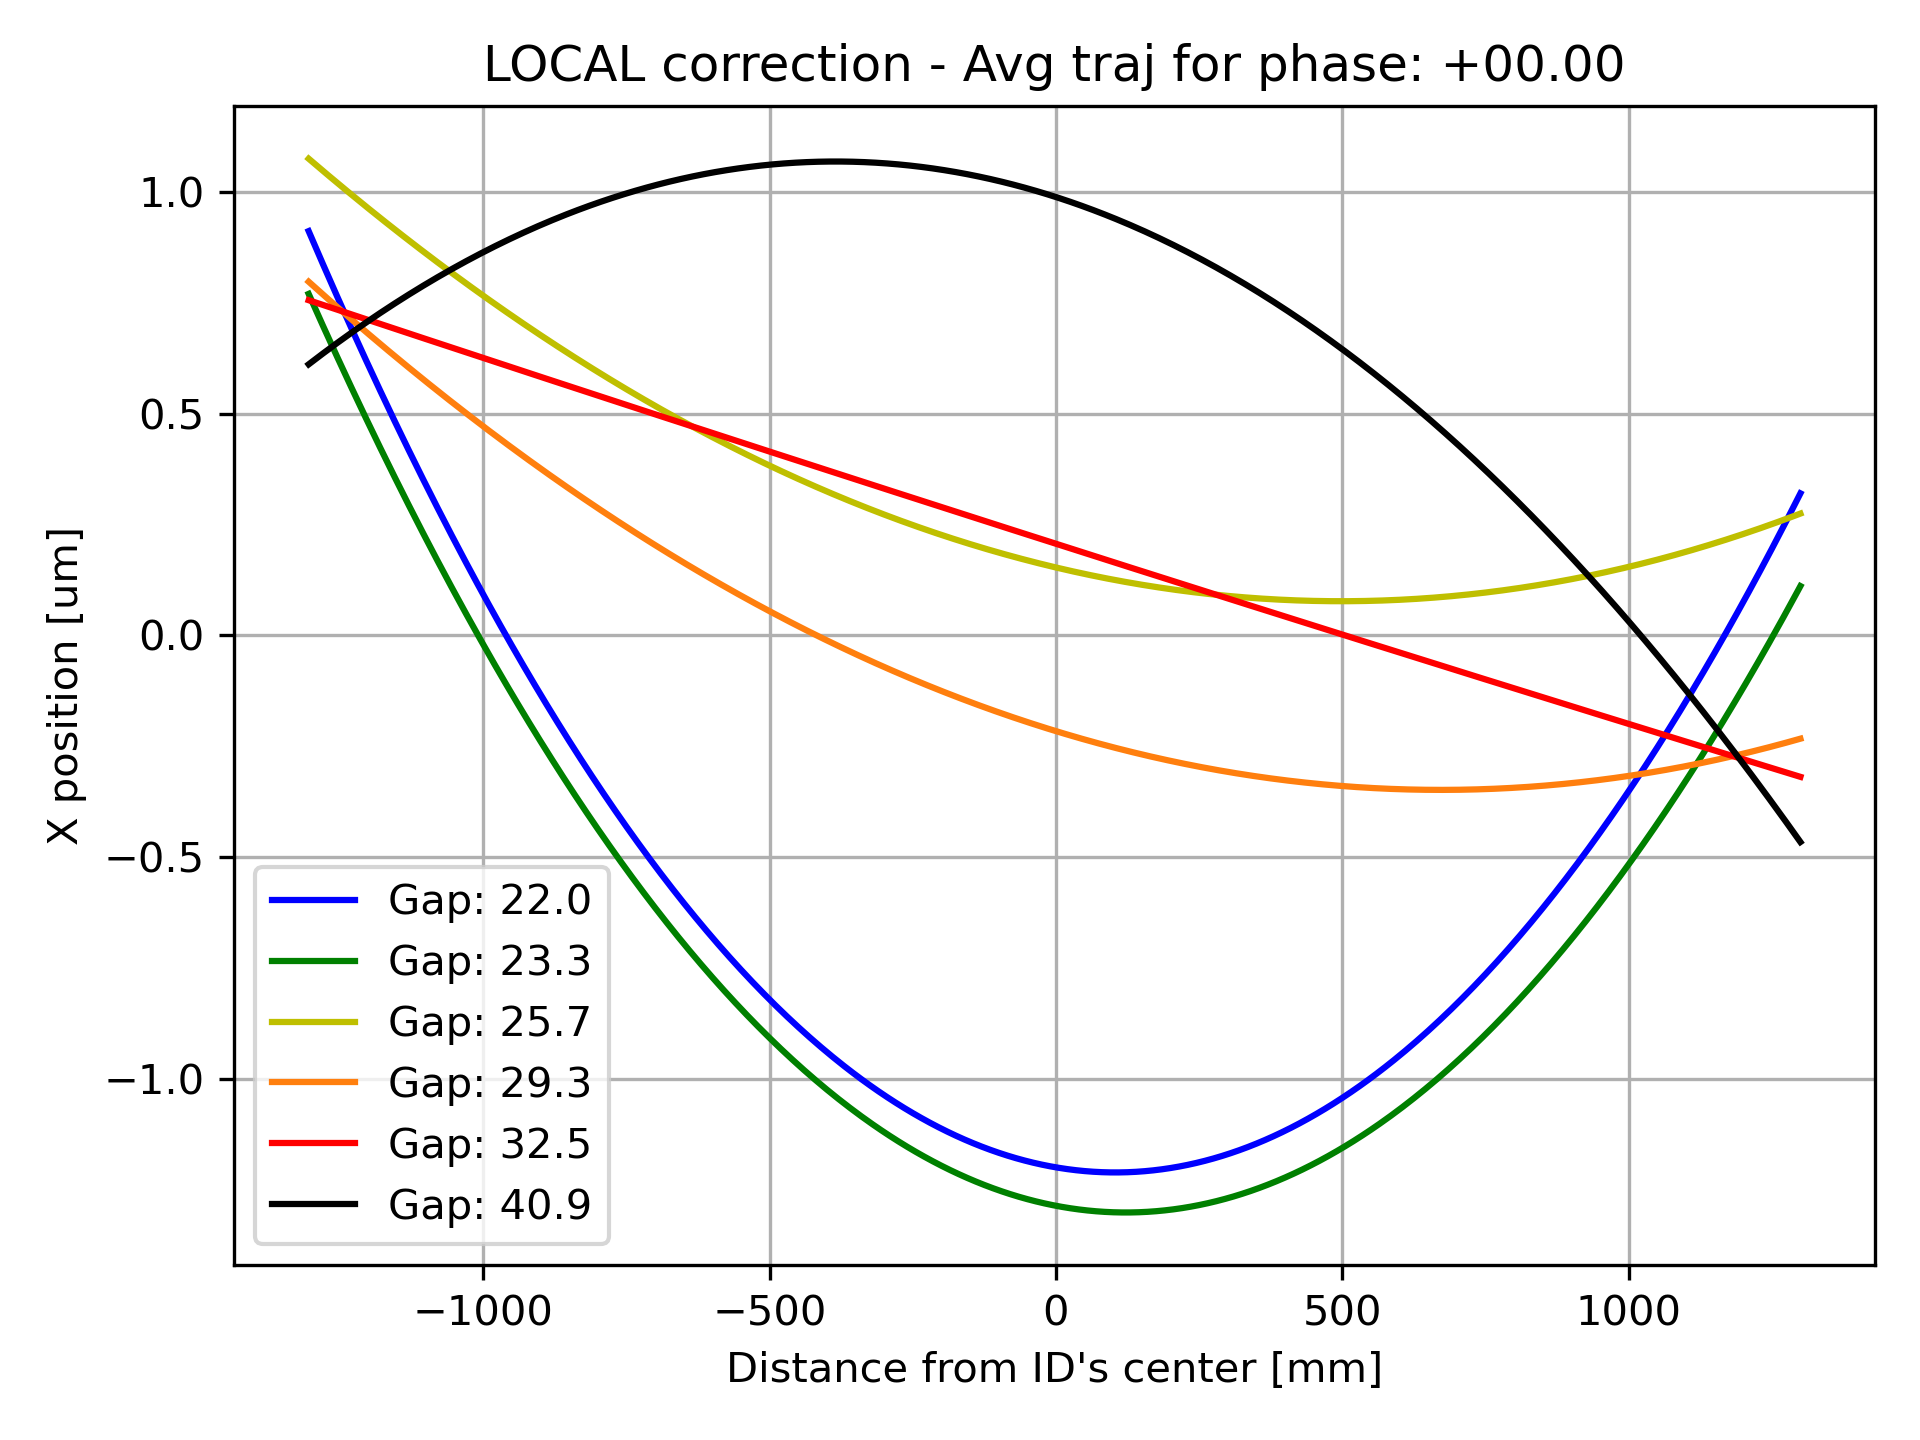
\includegraphics[width=0.9\linewidth, height=7cm]{figs/phase0 horizontal-avg-traj-LOCAL.png}
\label{fig:subim20xc}
\end{subfigure}
\caption{Trajetória média horizontal após correções de órbita utilizando FOFB (esquerda) e feedforward (direita)}
\label{fig:corrx}
\end{figure}

\begin{figure}[H]
\begin{subfigure}{0.5\textwidth}
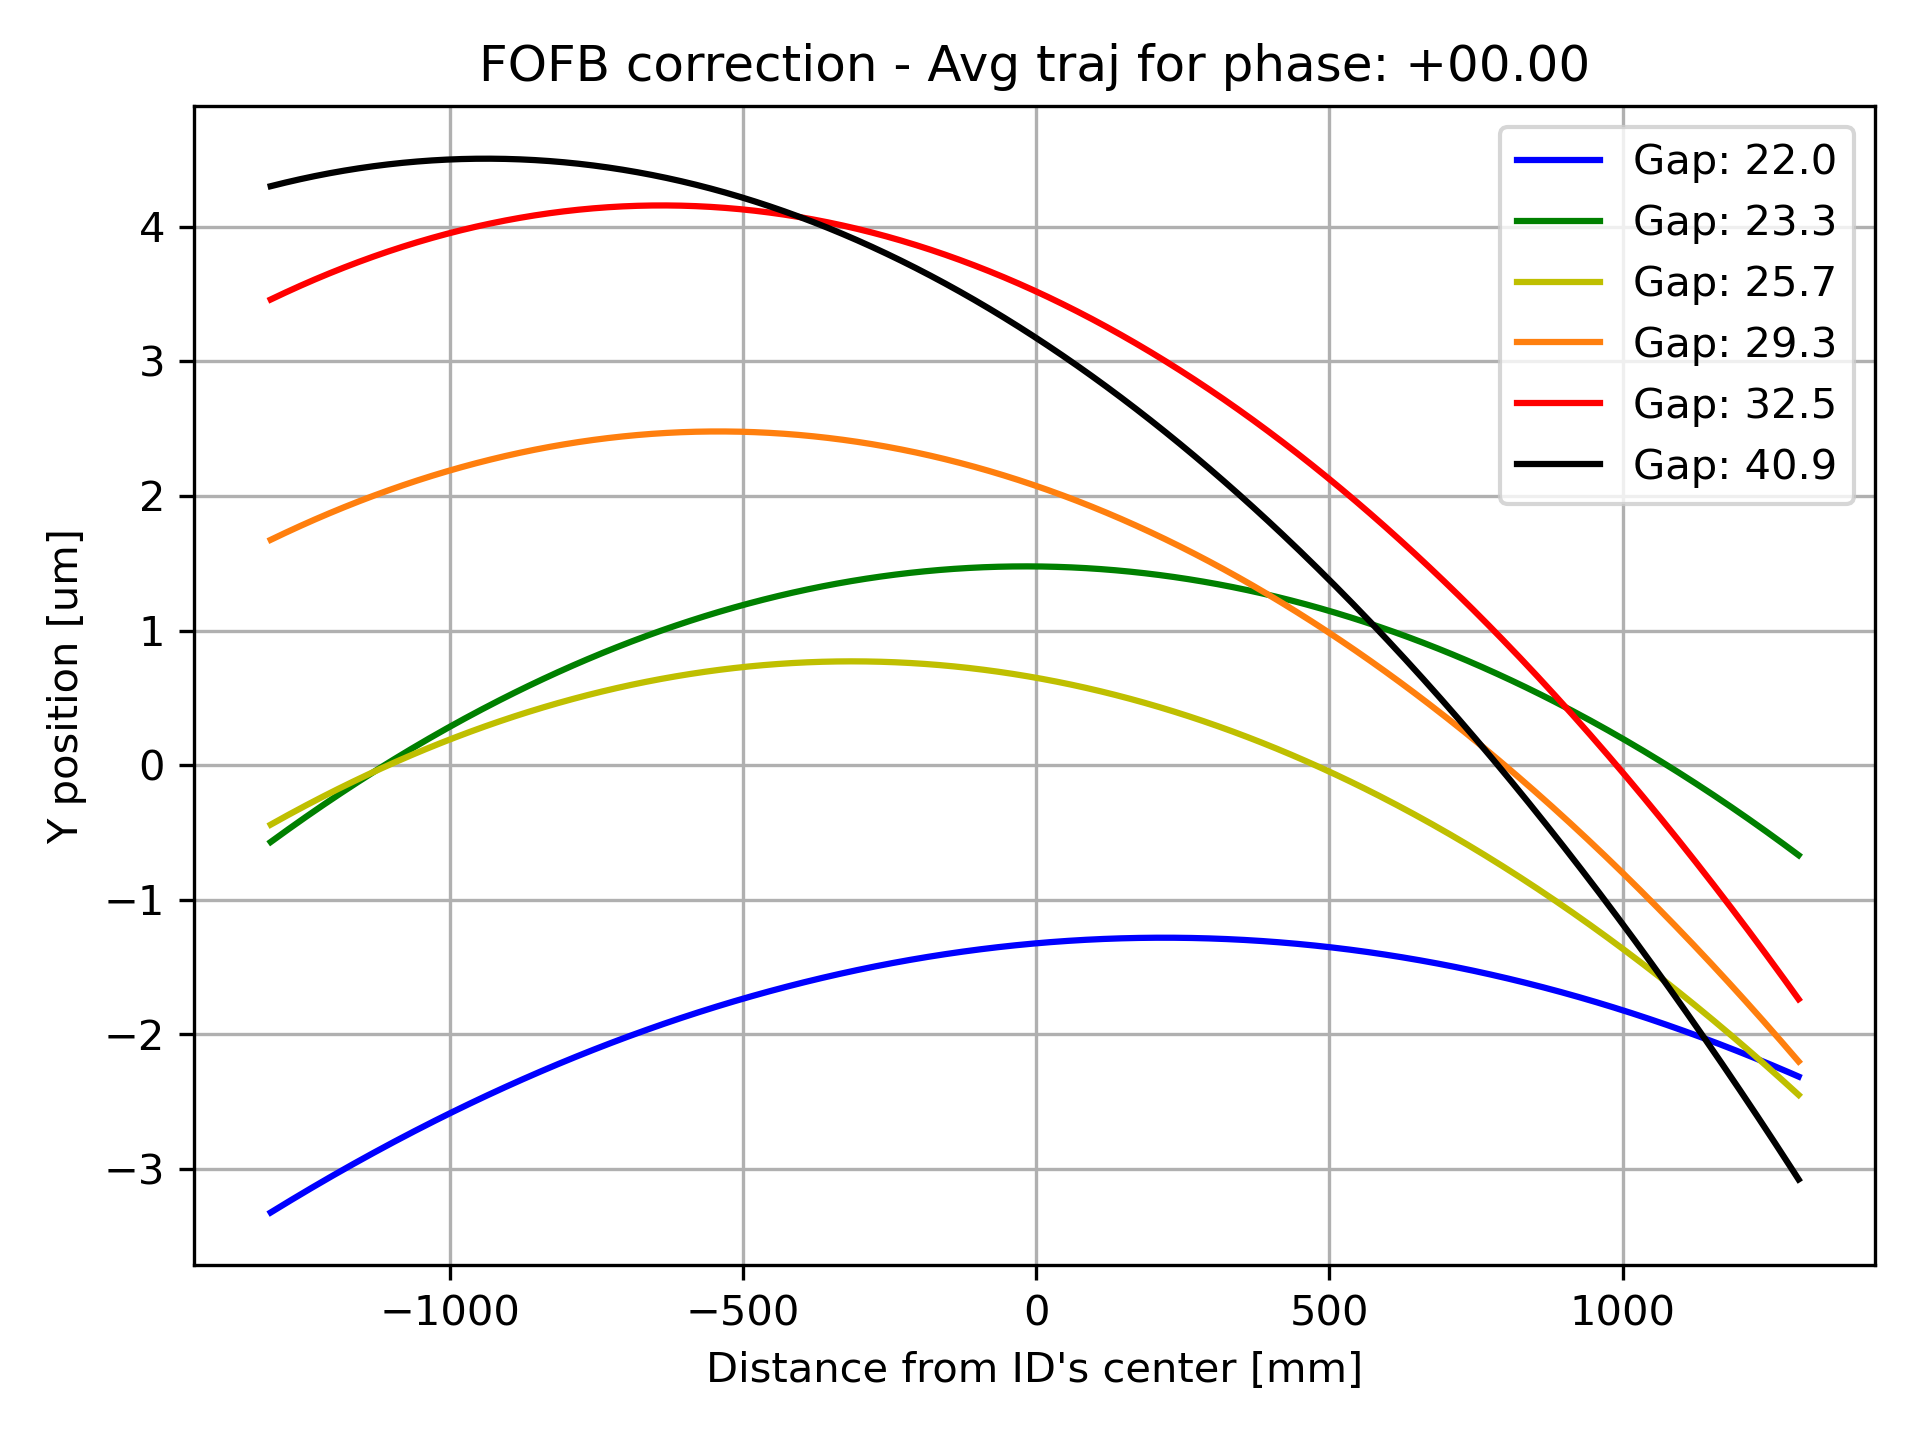
\includegraphics[width=0.9\linewidth, height=7cm]{figs/phase0 vertical-avg-traj-FOFB.png} 
\label{fig:subim10yc}
\end{subfigure}
\begin{subfigure}{0.5\textwidth}
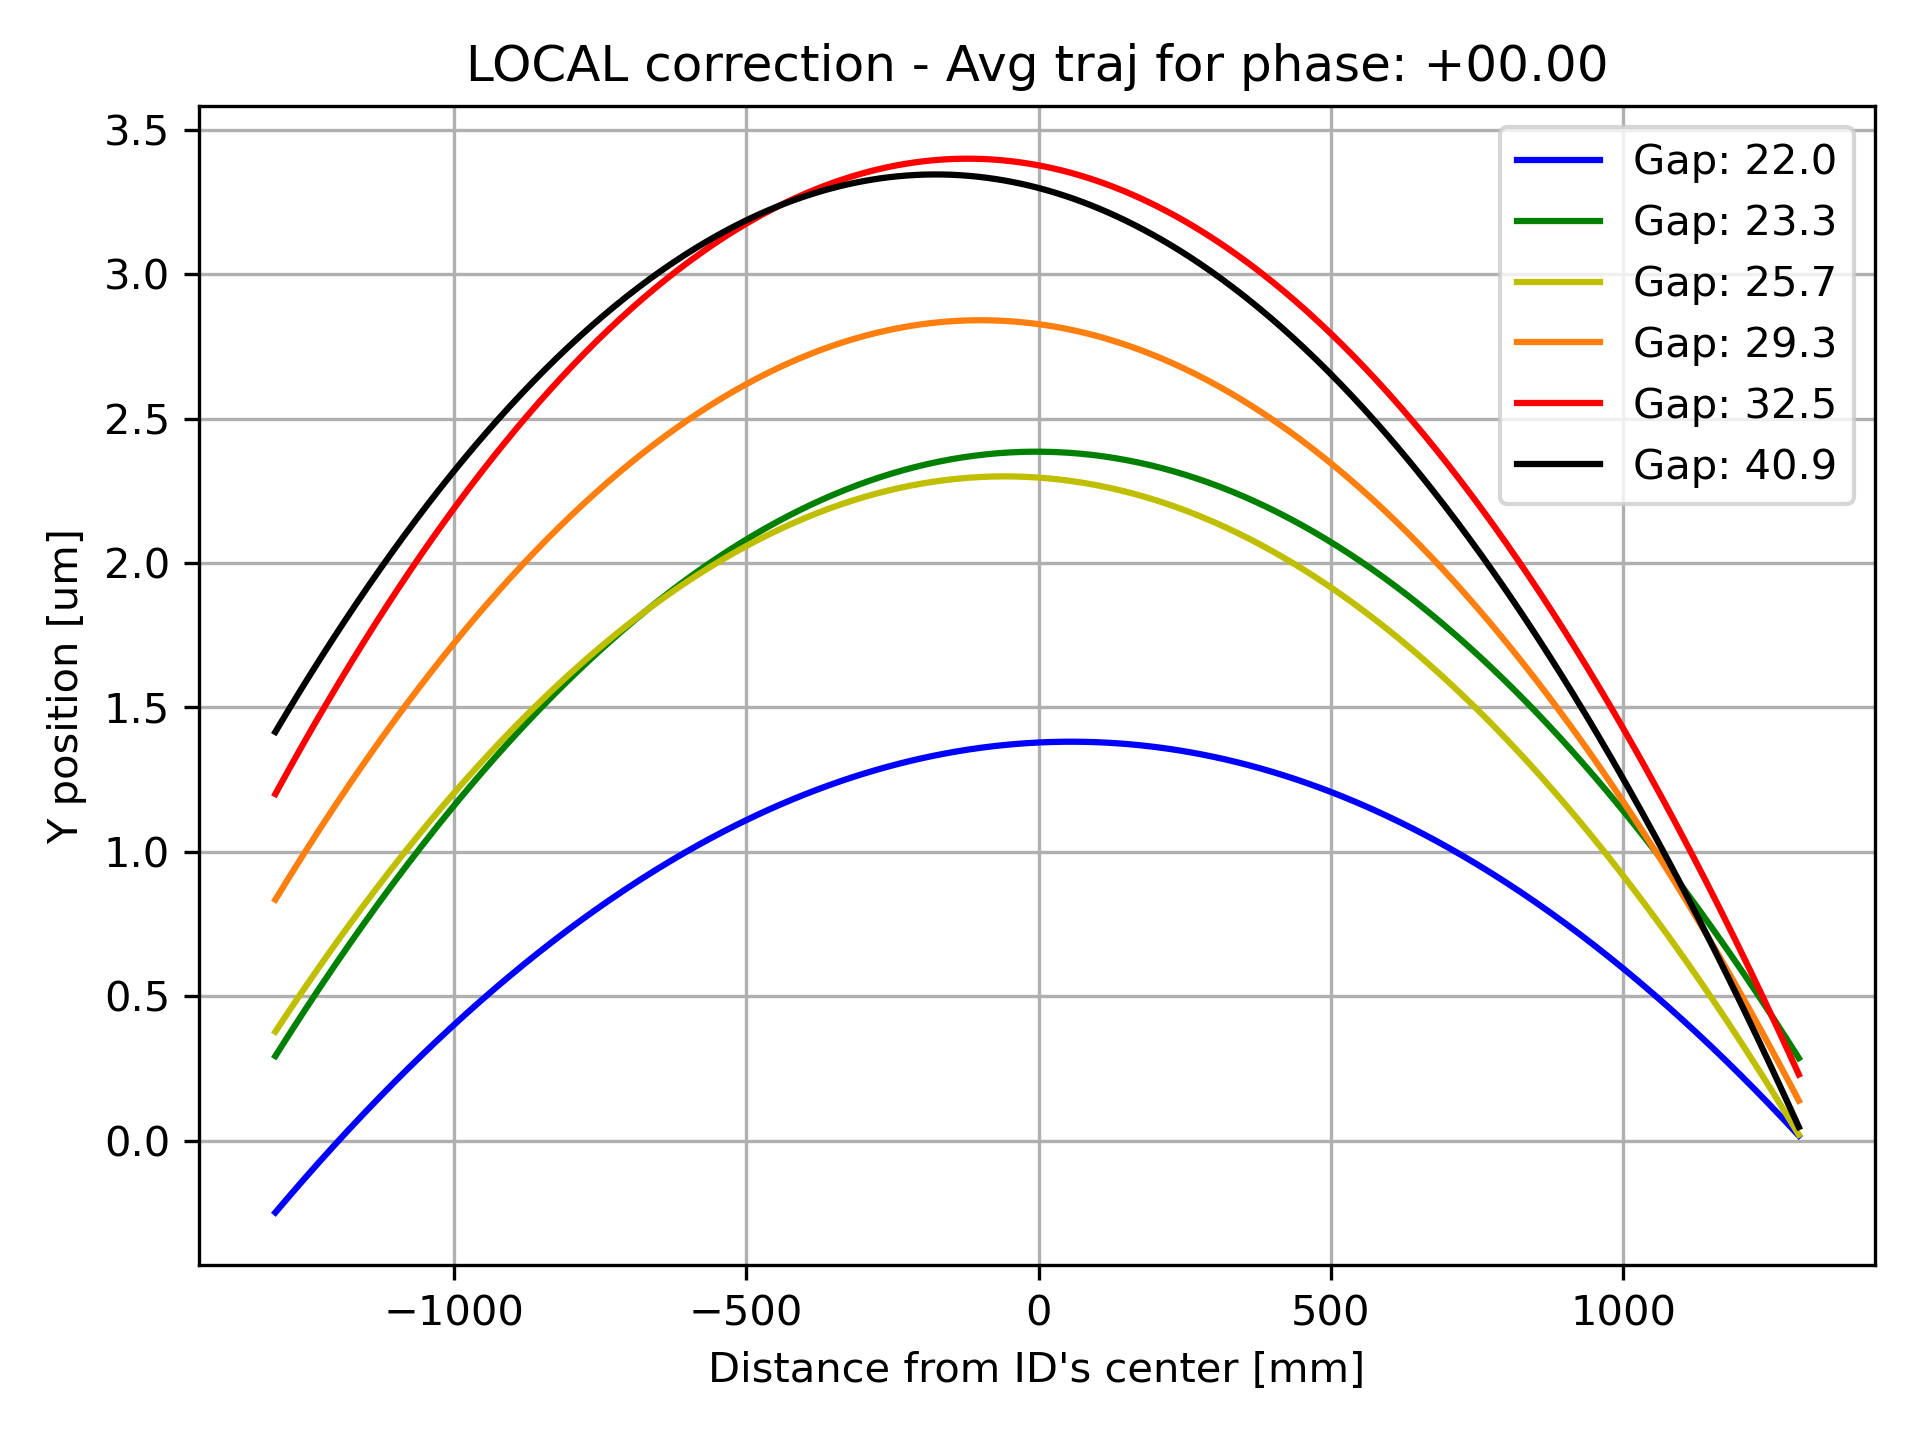
\includegraphics[width=0.9\linewidth, height=7cm]{figs/phase0 vertical-avg-traj-LOCAL.png}
\label{fig:subim20yc}
\end{subfigure}
\caption{Trajetória média vertical após correções de órbita utilizando FOFB (esquerda) e feedforward (direita)}
\label{fig:corry}
\end{figure}







\subsubsection{Trajetória}
As figuras abaixo exibem a trajetória do elétron no ID para diversos gaps, tanto em ângulo quanto em posição para ambas coordenadas transversais. Na legenda encontram-se os valores finais de ângulo e posição para cada gap.

\begin{figure}[H]
\begin{subfigure}{0.5\textwidth}
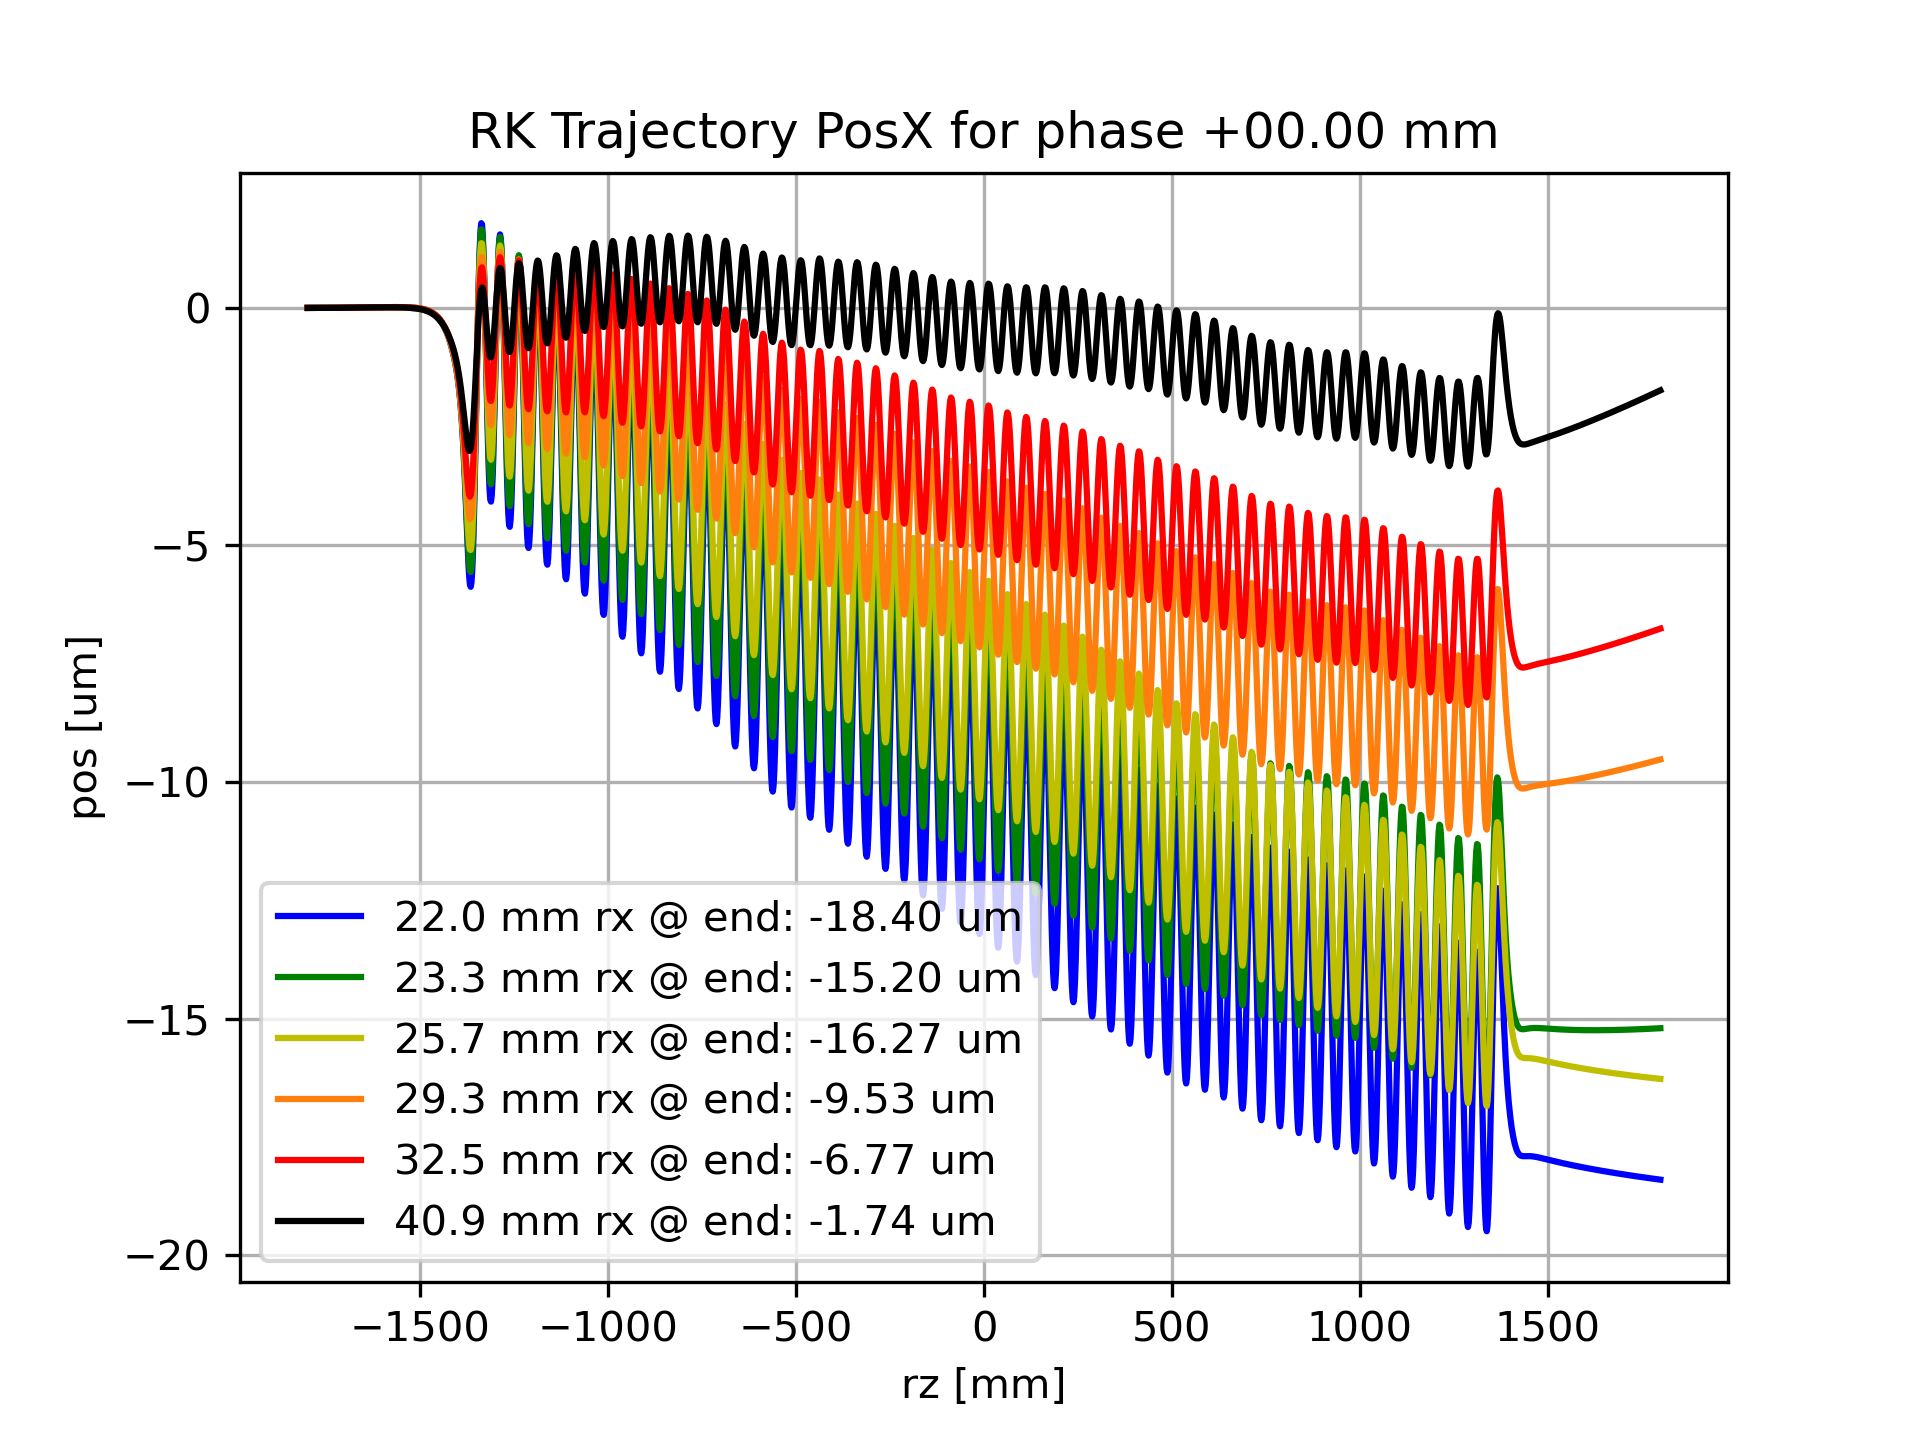
\includegraphics[width=0.9\linewidth, height=7cm]{figs/phase0 RK Posx.png} 
\label{fig:subim10tx}
\end{subfigure}
\begin{subfigure}{0.5\textwidth}
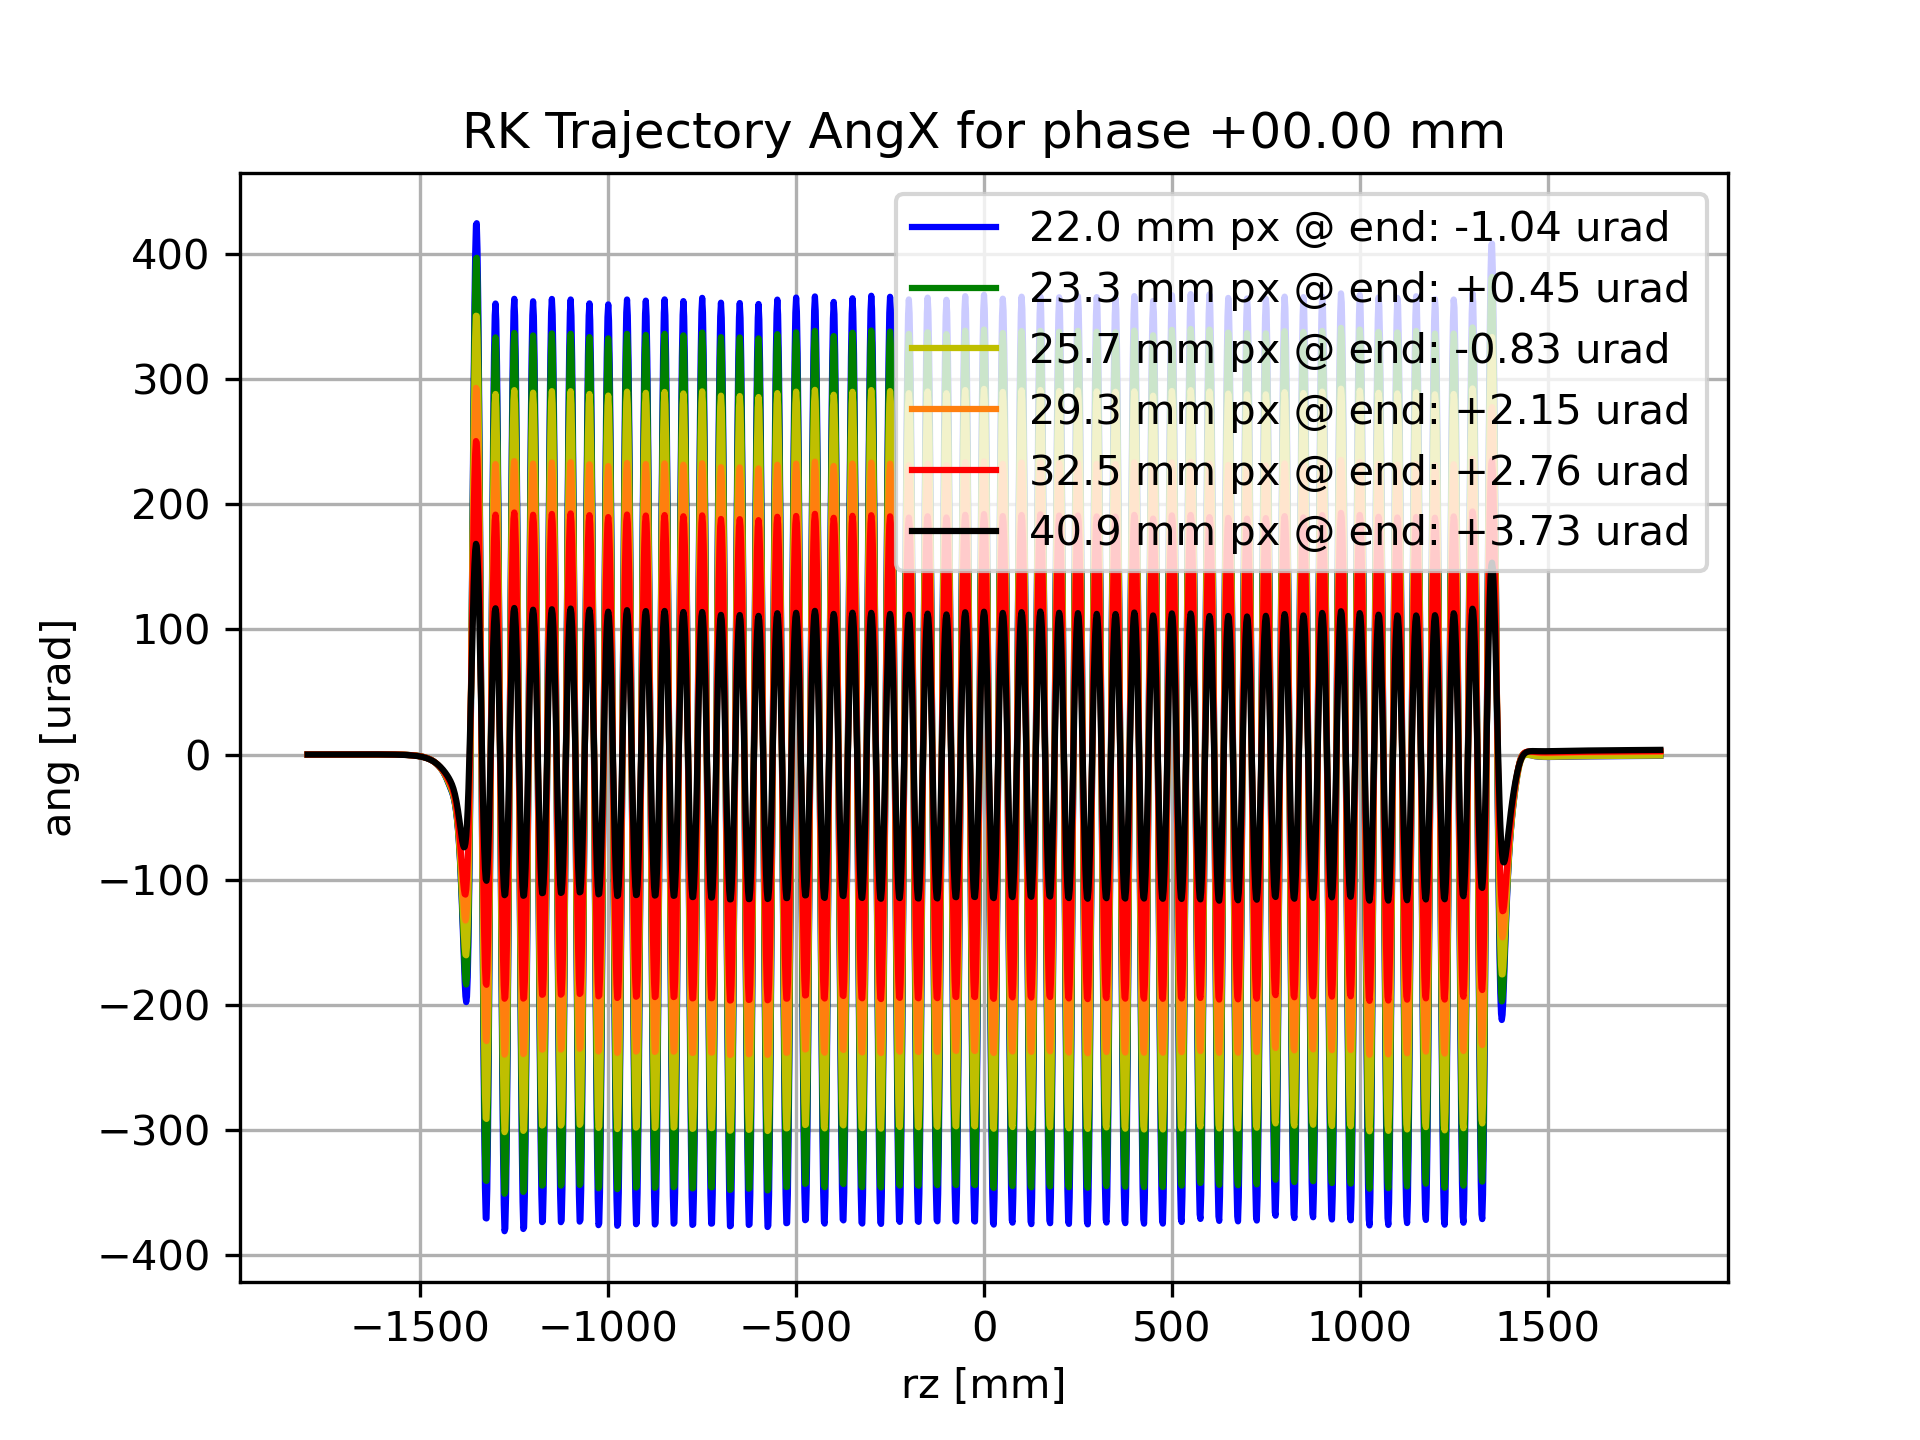
\includegraphics[width=0.9\linewidth, height=7cm]{figs/phase0 RK Angx.png}
\label{fig:subim20tx}
\end{subfigure}
\caption{Trajetória X para fase 00.00 mm}
\label{fig:trajx0}
\end{figure}

\begin{figure}[H]
\begin{subfigure}{0.5\textwidth}
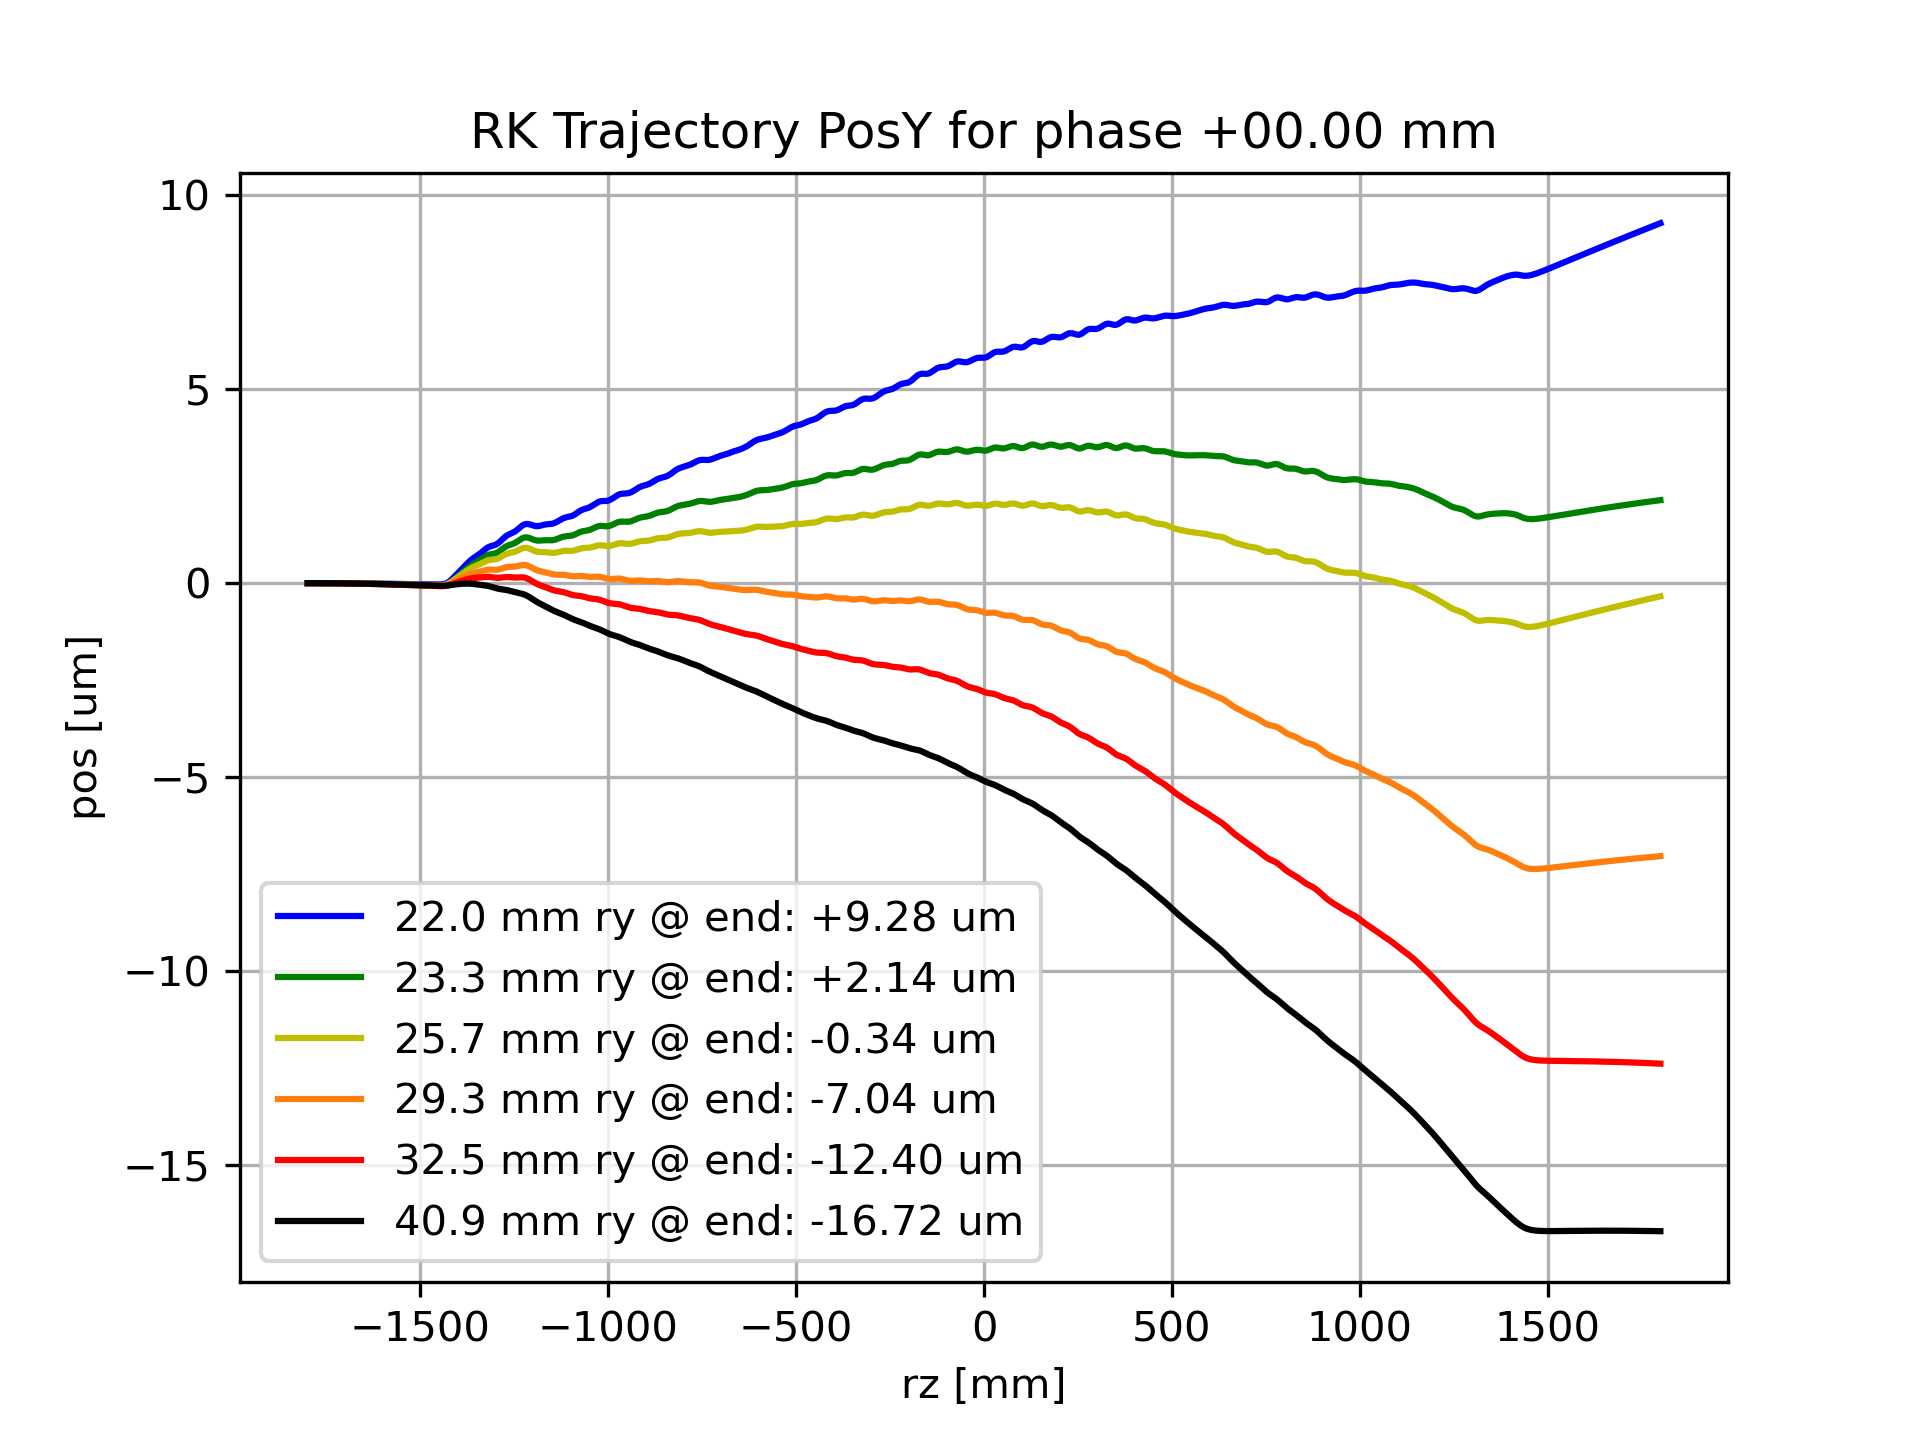
\includegraphics[width=0.9\linewidth, height=7cm]{figs/phase0 RK Posy.png} 
\label{fig:subim10ty}
\end{subfigure}
\begin{subfigure}{0.5\textwidth}
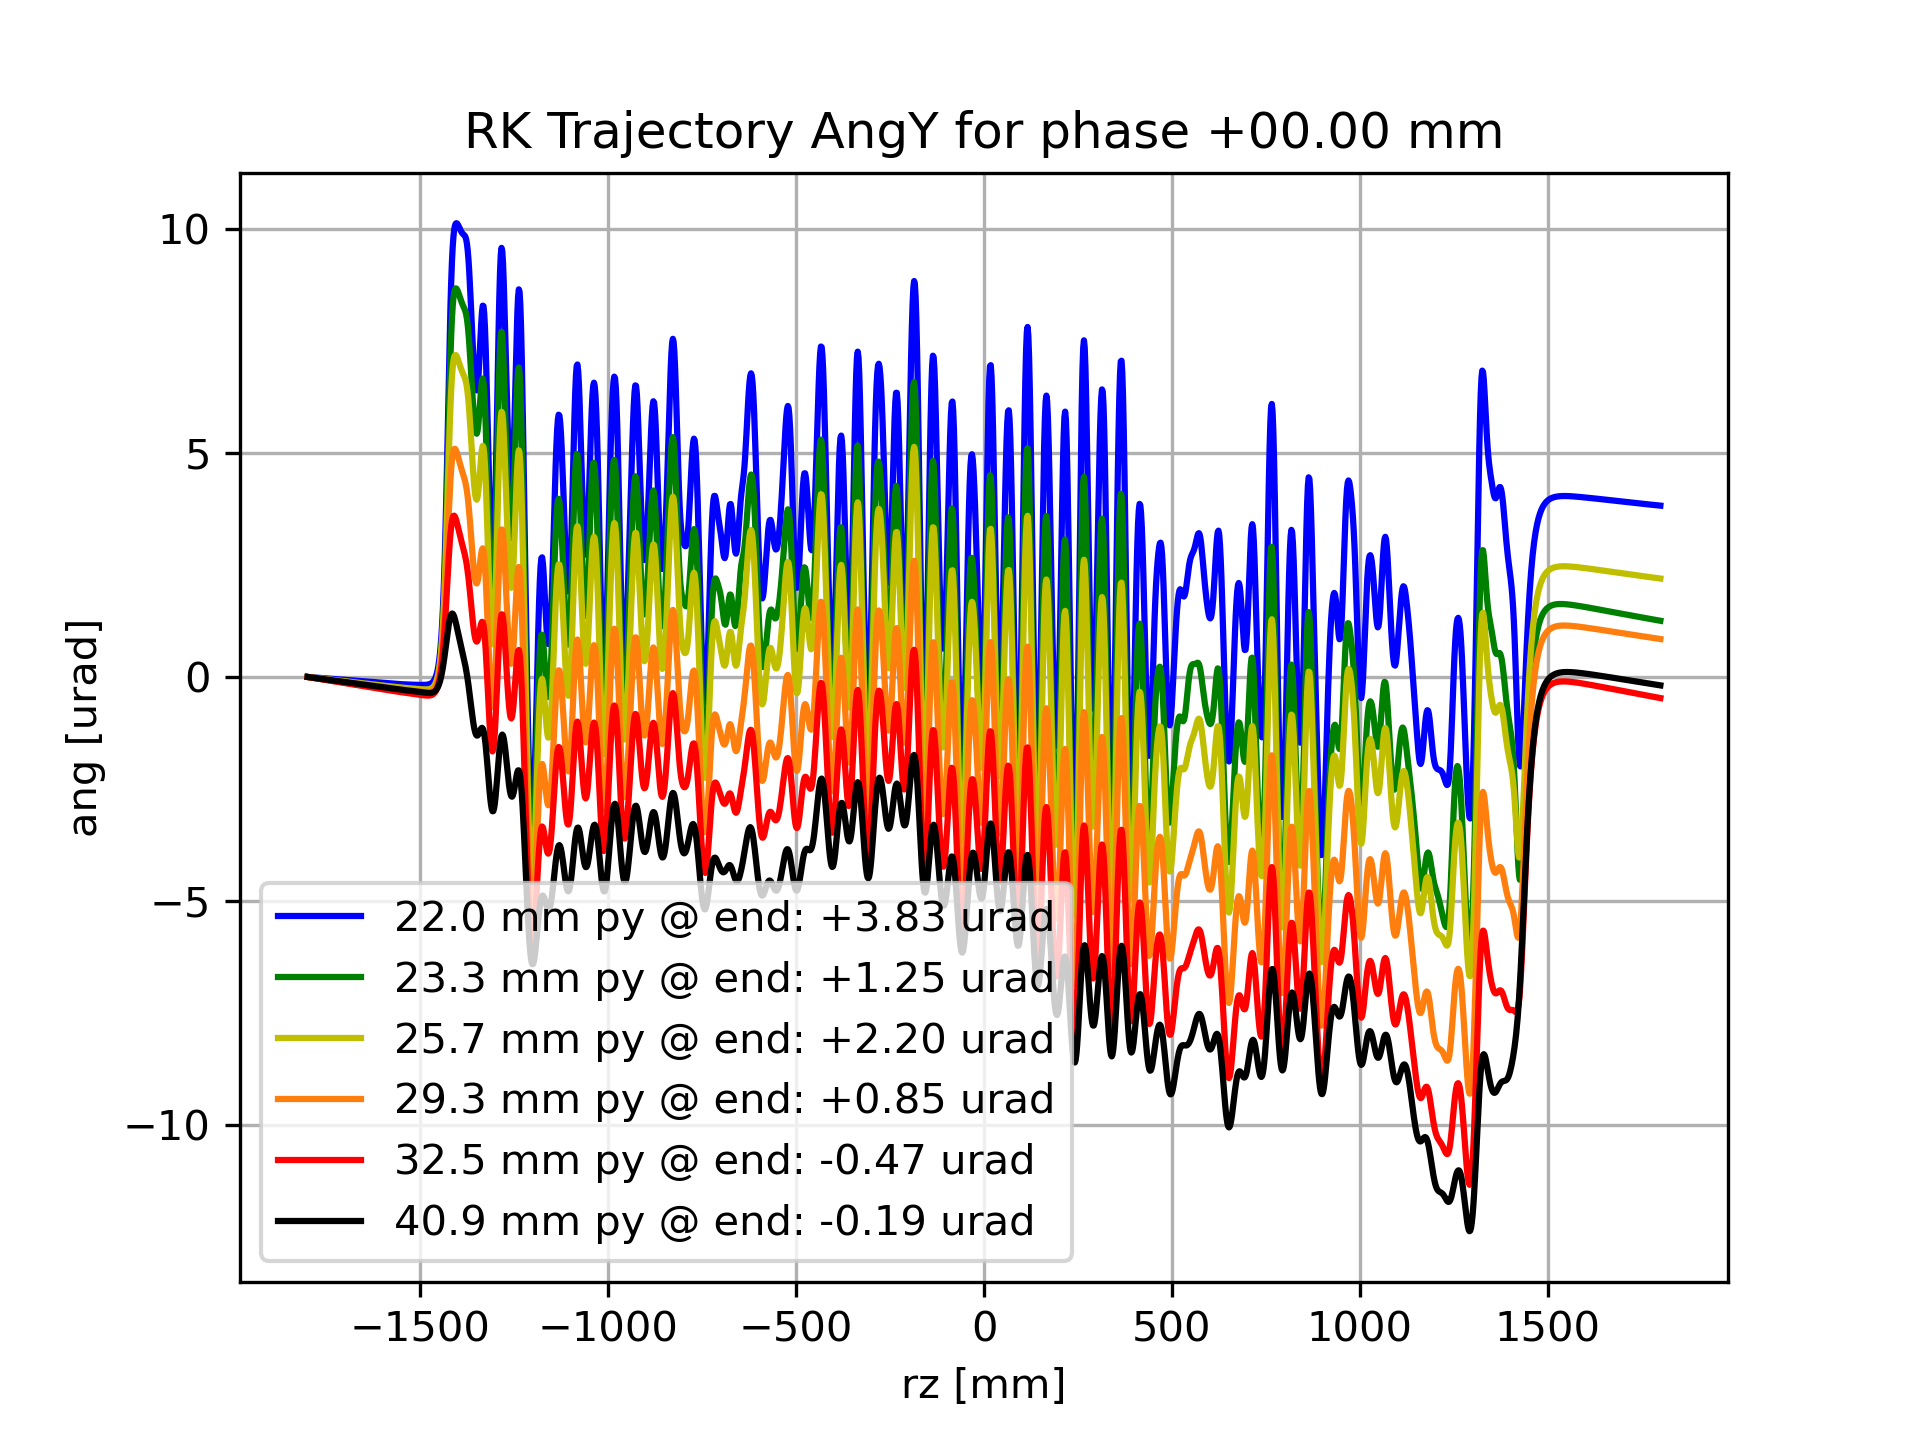
\includegraphics[width=0.9\linewidth, height=7cm]{figs/phase0 RK Angy.png}
\label{fig:subim20ty}
\end{subfigure}
\caption{Trajetória Y para fase 00.00 mm}
\label{fig:trajy0}
\end{figure}

Os valores finais de ângulo e trajetória mostrados nas figuras acima estão resumidos nas tabelas abaixo, em conjunto com as integrais de campo.


\begin{table}[H]
\centering
\caption{Primeiras integrais de campo}
\begin{tabular}{|c|c|c|}
\hline
   Gap [mm] & Bx 1st integral [G cm] / $\Delta$ py [$\mu$rad] & By 1st integral [G cm] / $\Delta$ px [$\mu$rad] \\
\hline
    22.0 & -37.8 / +3.83 & -10.5 / -1.04 \\
    23.3 & -12.7 / +1.25 &  +4.5 / +0.45 \\
    25.7 & -21.7 / +2.20 &  -8.3 / -0.83 \\
    29.3 &  -8.4 / +0.85 & +21.5 / +2.15 \\
    32.5 &  +4.7 / -0.47 & +27.6 / +2.76 \\
    40.9 &  +1.9 / -0.19 & +37.3 / +3.73 \\
\hline
\end{tabular}
\end{table}

\begin{table}[H]
\centering
\caption{Segundas integrais de campo}
\begin{tabular}{|c|c|c|}
\hline
   Gap [mm] & Bx 2nd integral [G cm²] / $\Delta$ y [$\mu$m] & By 2nd integral [G cm²] / $\Delta$ x [$\mu$m]   \\
\hline
    22.0 & -9.18e+03 / +9.28 & -1.84e+04 / -18.40 \\
    23.3 & -2.14e+03 / +2.14 & -1.52e+04 / -15.20 \\
    25.7 & +3.93e+02 / -0.34 & -1.63e+04 / -16.27 \\
    29.3 & +7.06e+03 / -7.04 & -9.53e+03 / -9.53 \\
    32.5 & +1.24e+04 / -12.40 & -6.77e+03 / -6.77 \\
    40.9 & +1.67e+04 / -16.72 & -1.74e+03 / -1.74 \\
\hline
\end{tabular}
\end{table}

\subsubsection{Multipolos}
As figuras abaixo exibem os multipolos ao longo da trajetória do elétron no ID para diversos gaps.

\begin{figure}[H]
\begin{subfigure}{0.5\textwidth}
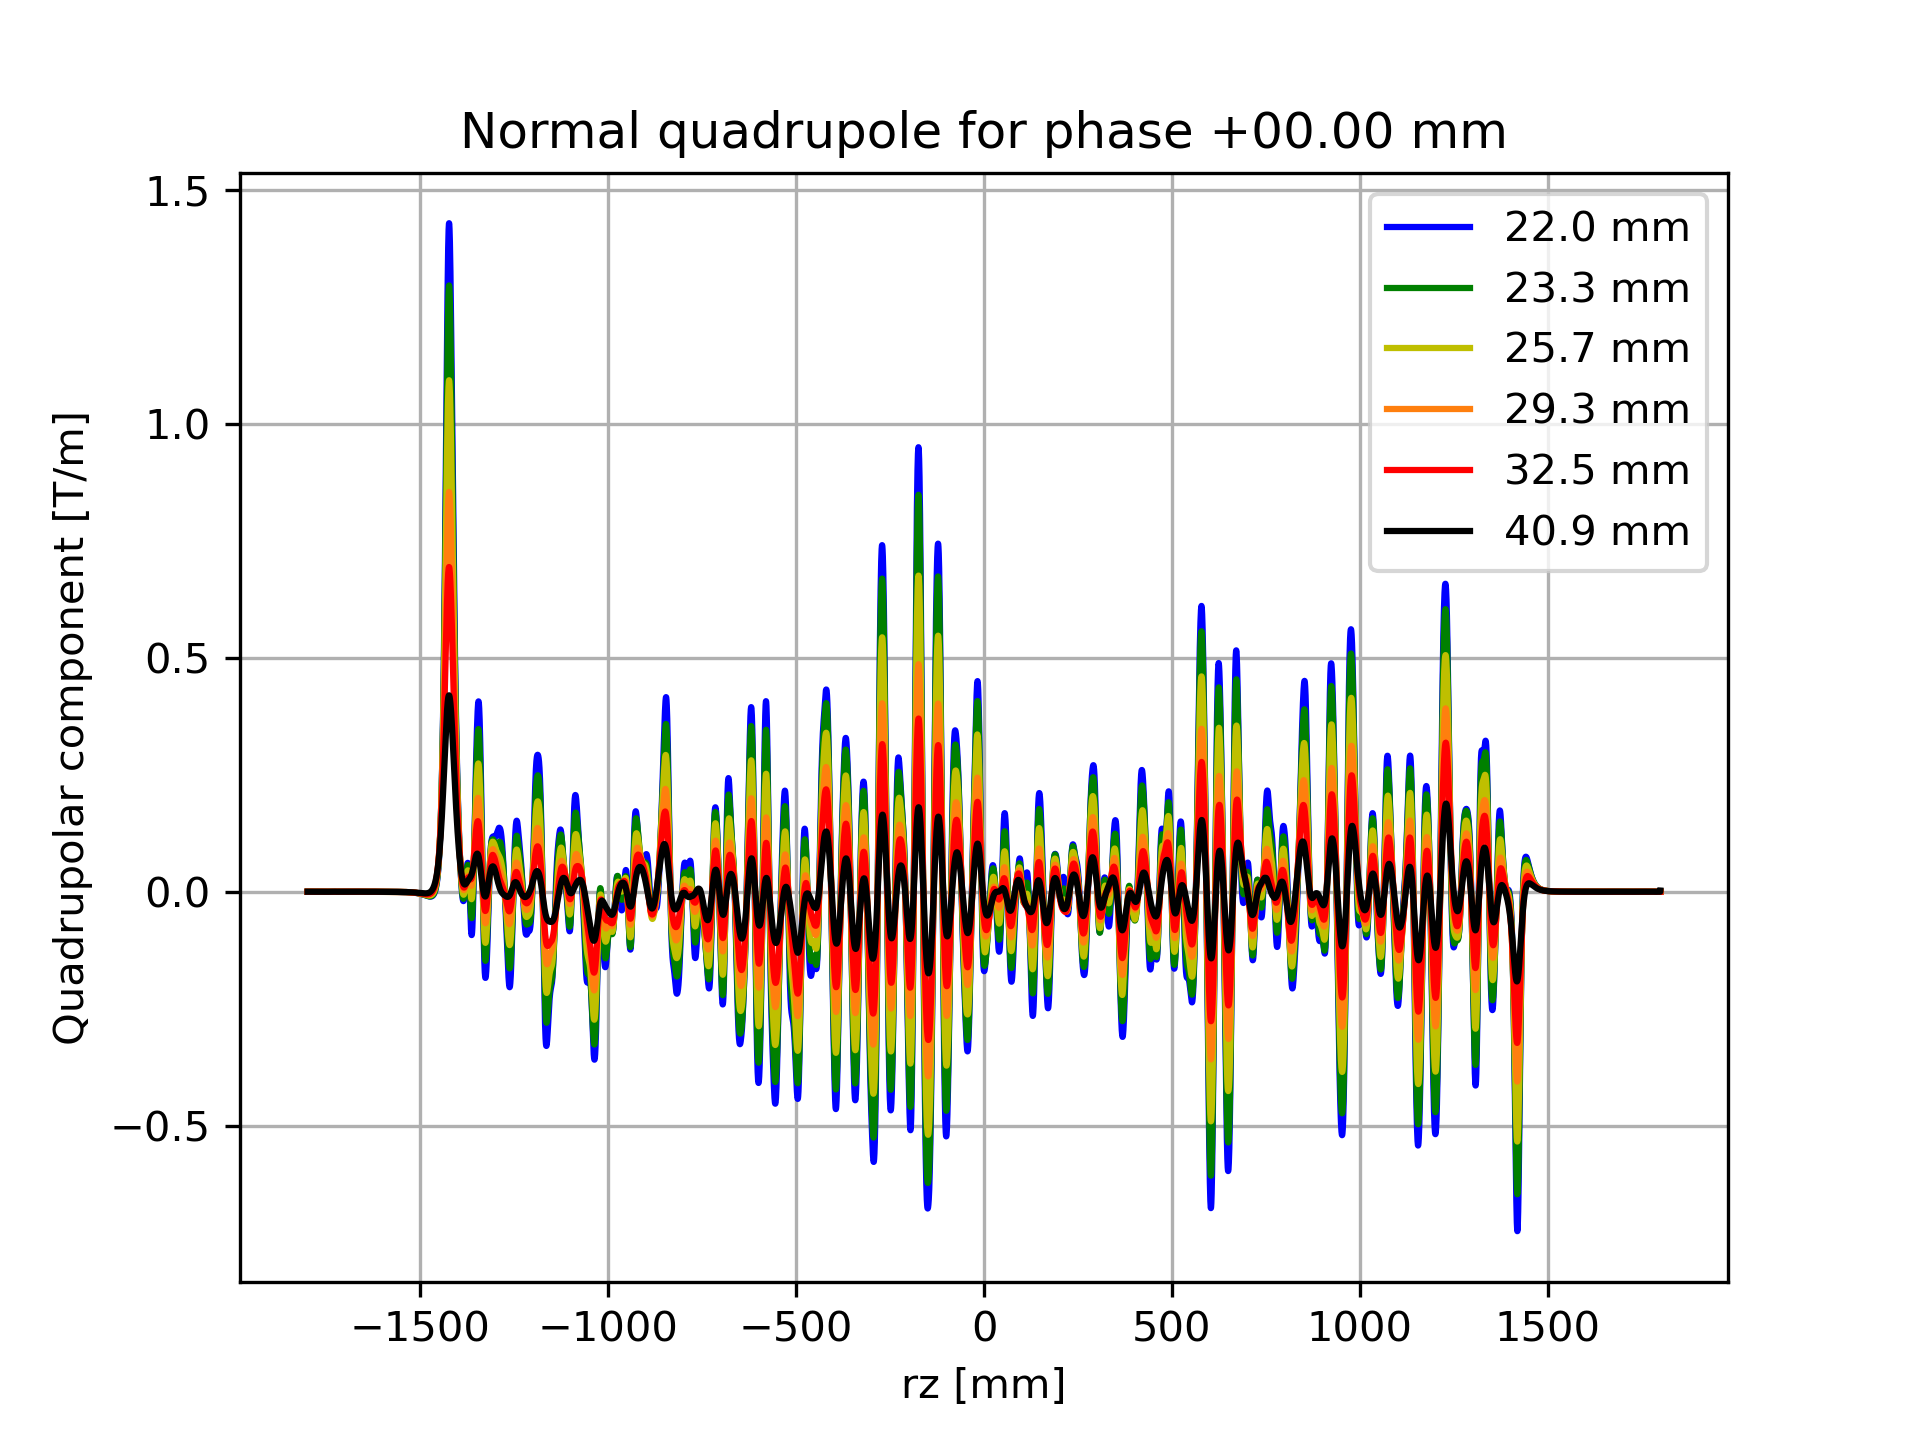
\includegraphics[width=0.9\linewidth, height=7cm]{figs/phase0 Normal quadrupole.png} 
\label{fig:subim10q}
\end{subfigure}
\begin{subfigure}{0.5\textwidth}
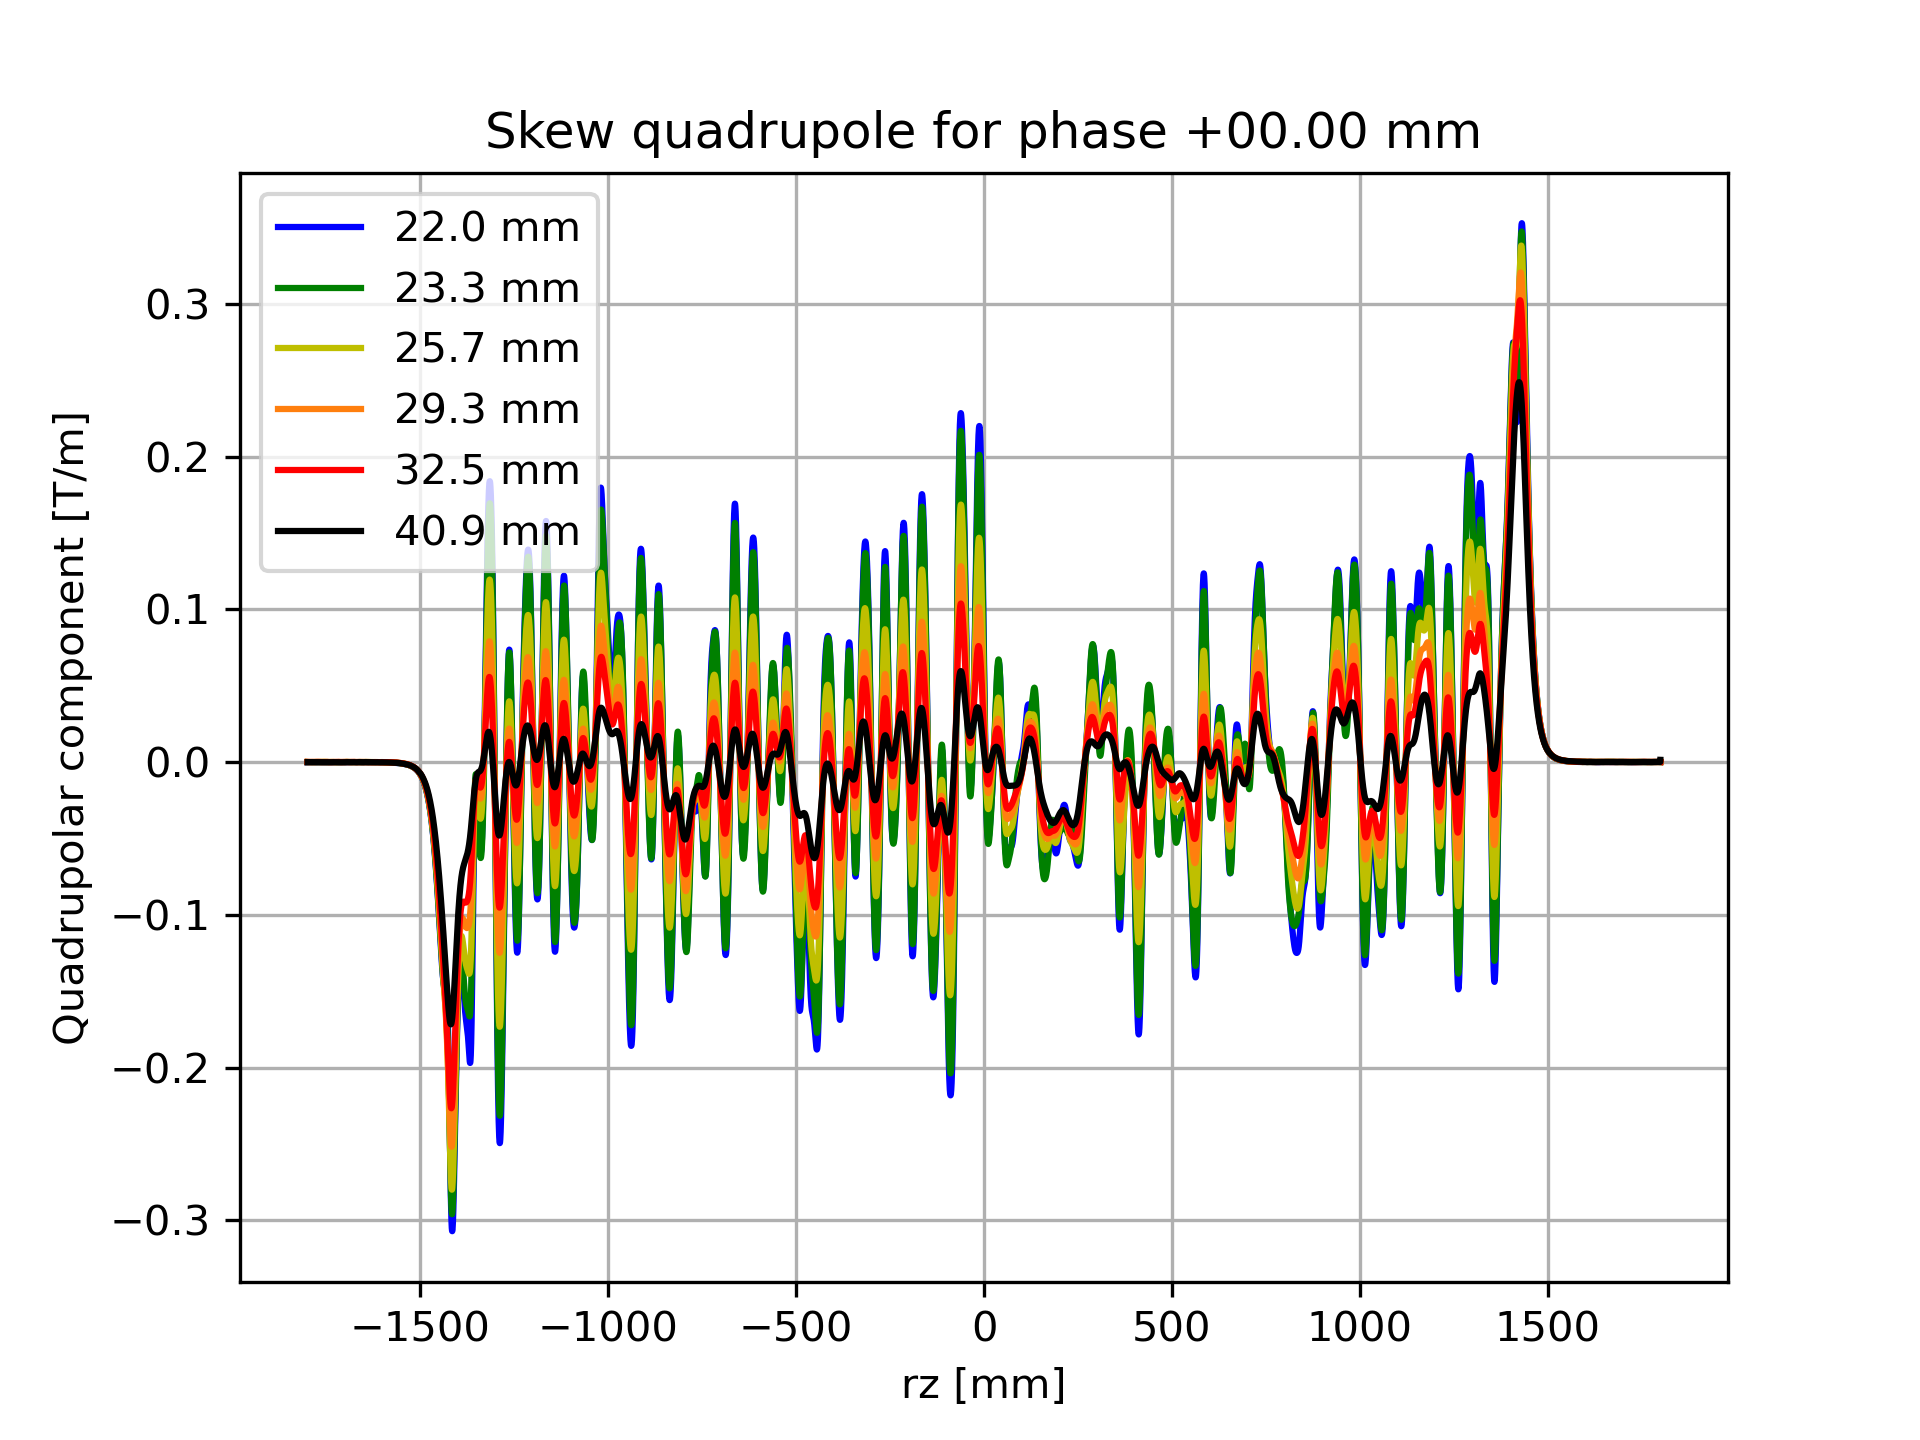
\includegraphics[width=0.9\linewidth, height=7cm]{figs/phase0 Skew quadrupole.png}
\label{fig:subim20q}
\end{subfigure}
\caption{Componentes quadrupolares de campo}
\label{fig:quad0}
\end{figure}

\begin{figure}[H]
\begin{subfigure}{0.5\textwidth}
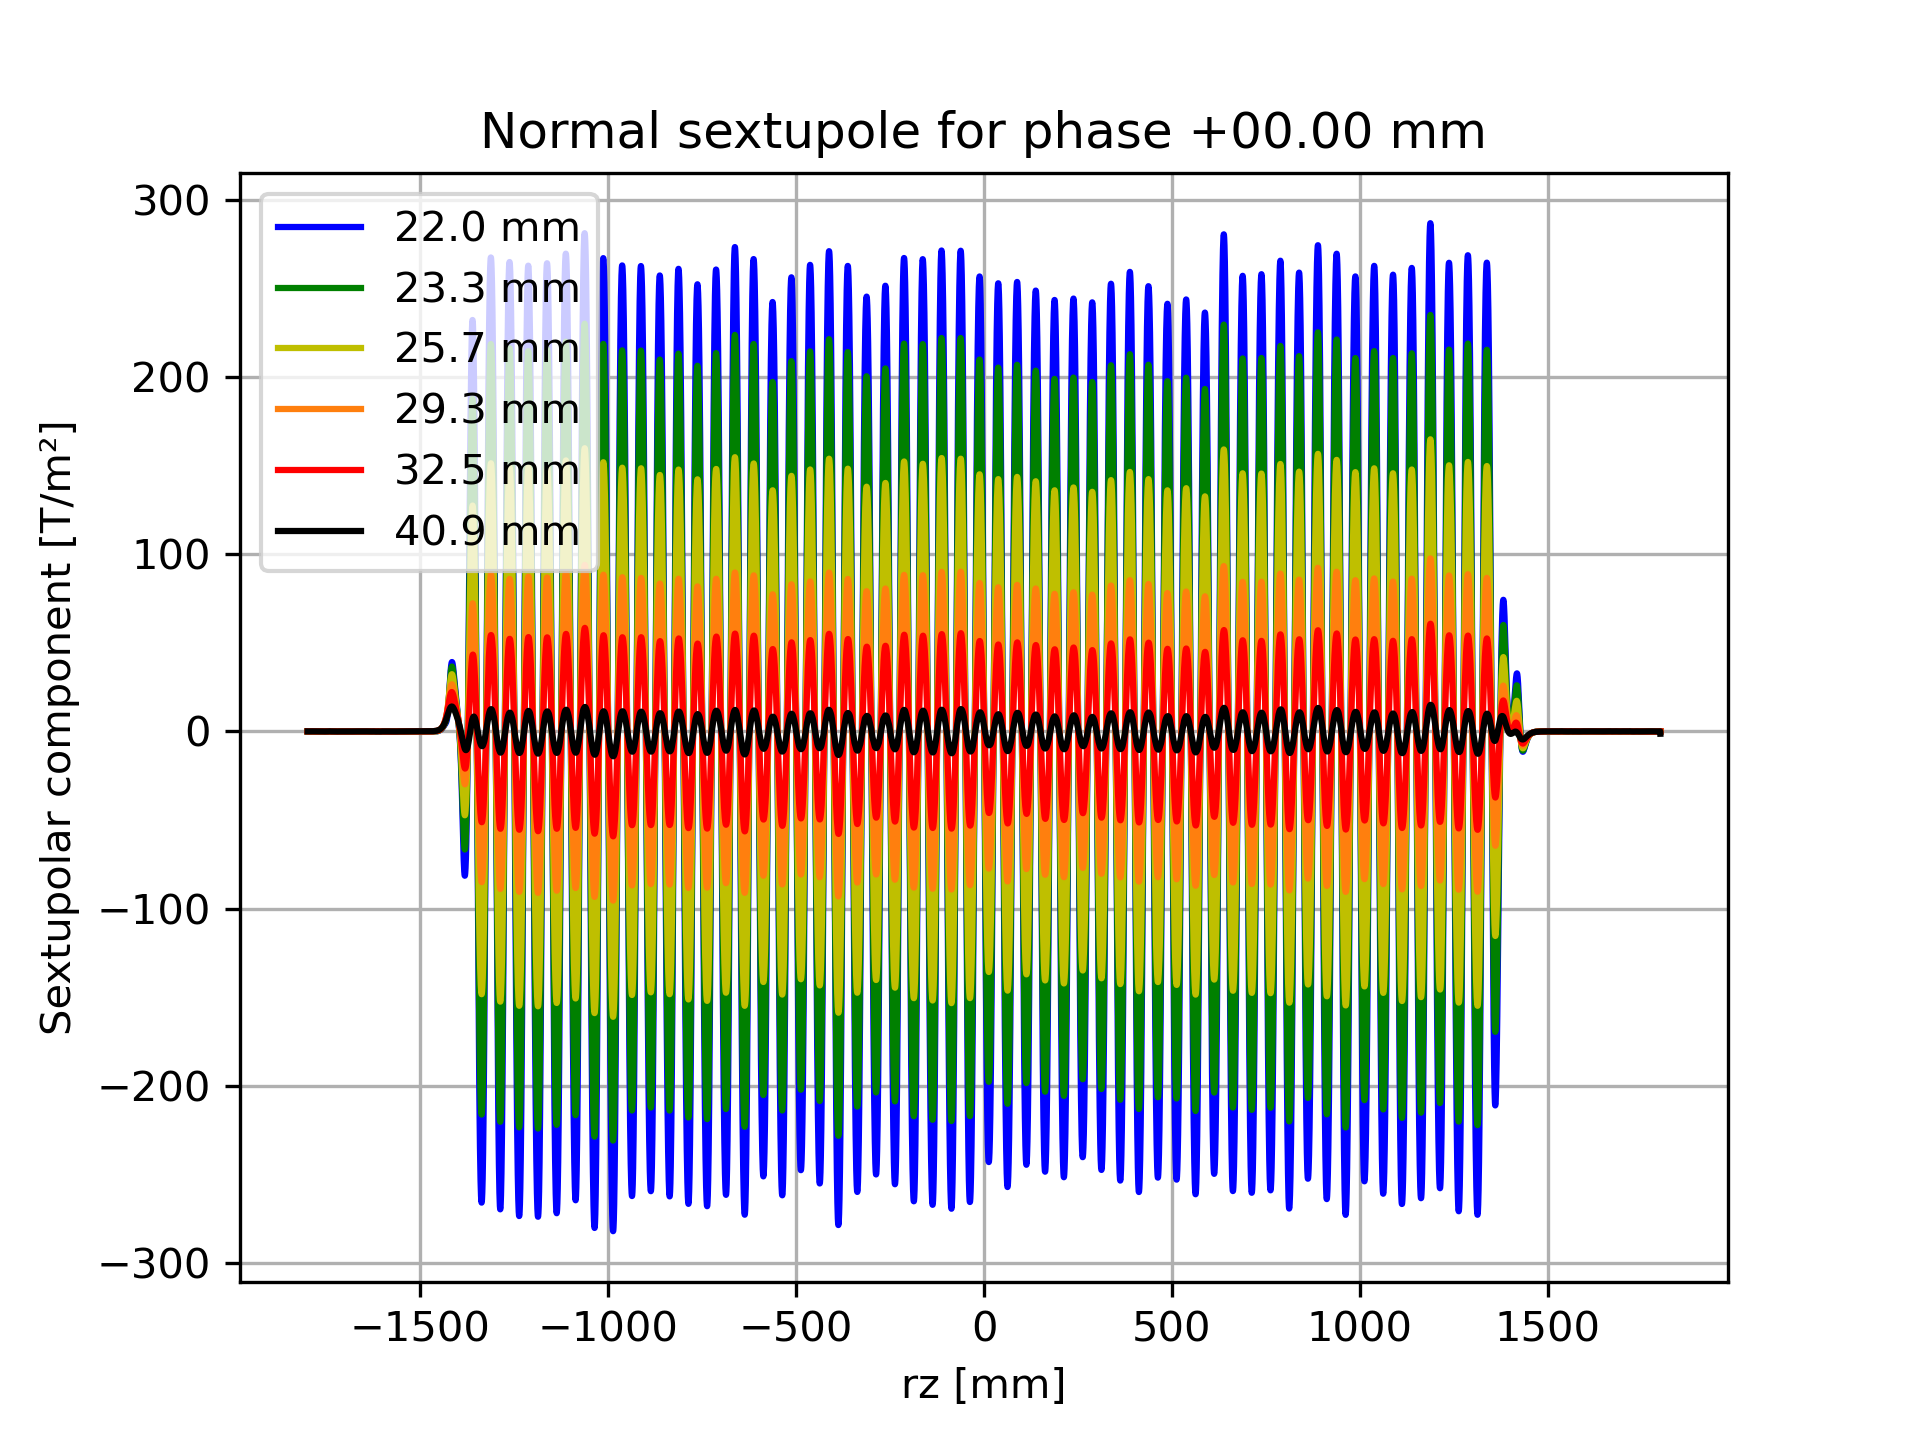
\includegraphics[width=0.9\linewidth, height=7cm]{figs/phase0 Normal sextupole.png} 
\label{fig:subim10s}
\end{subfigure}
\begin{subfigure}{0.5\textwidth}
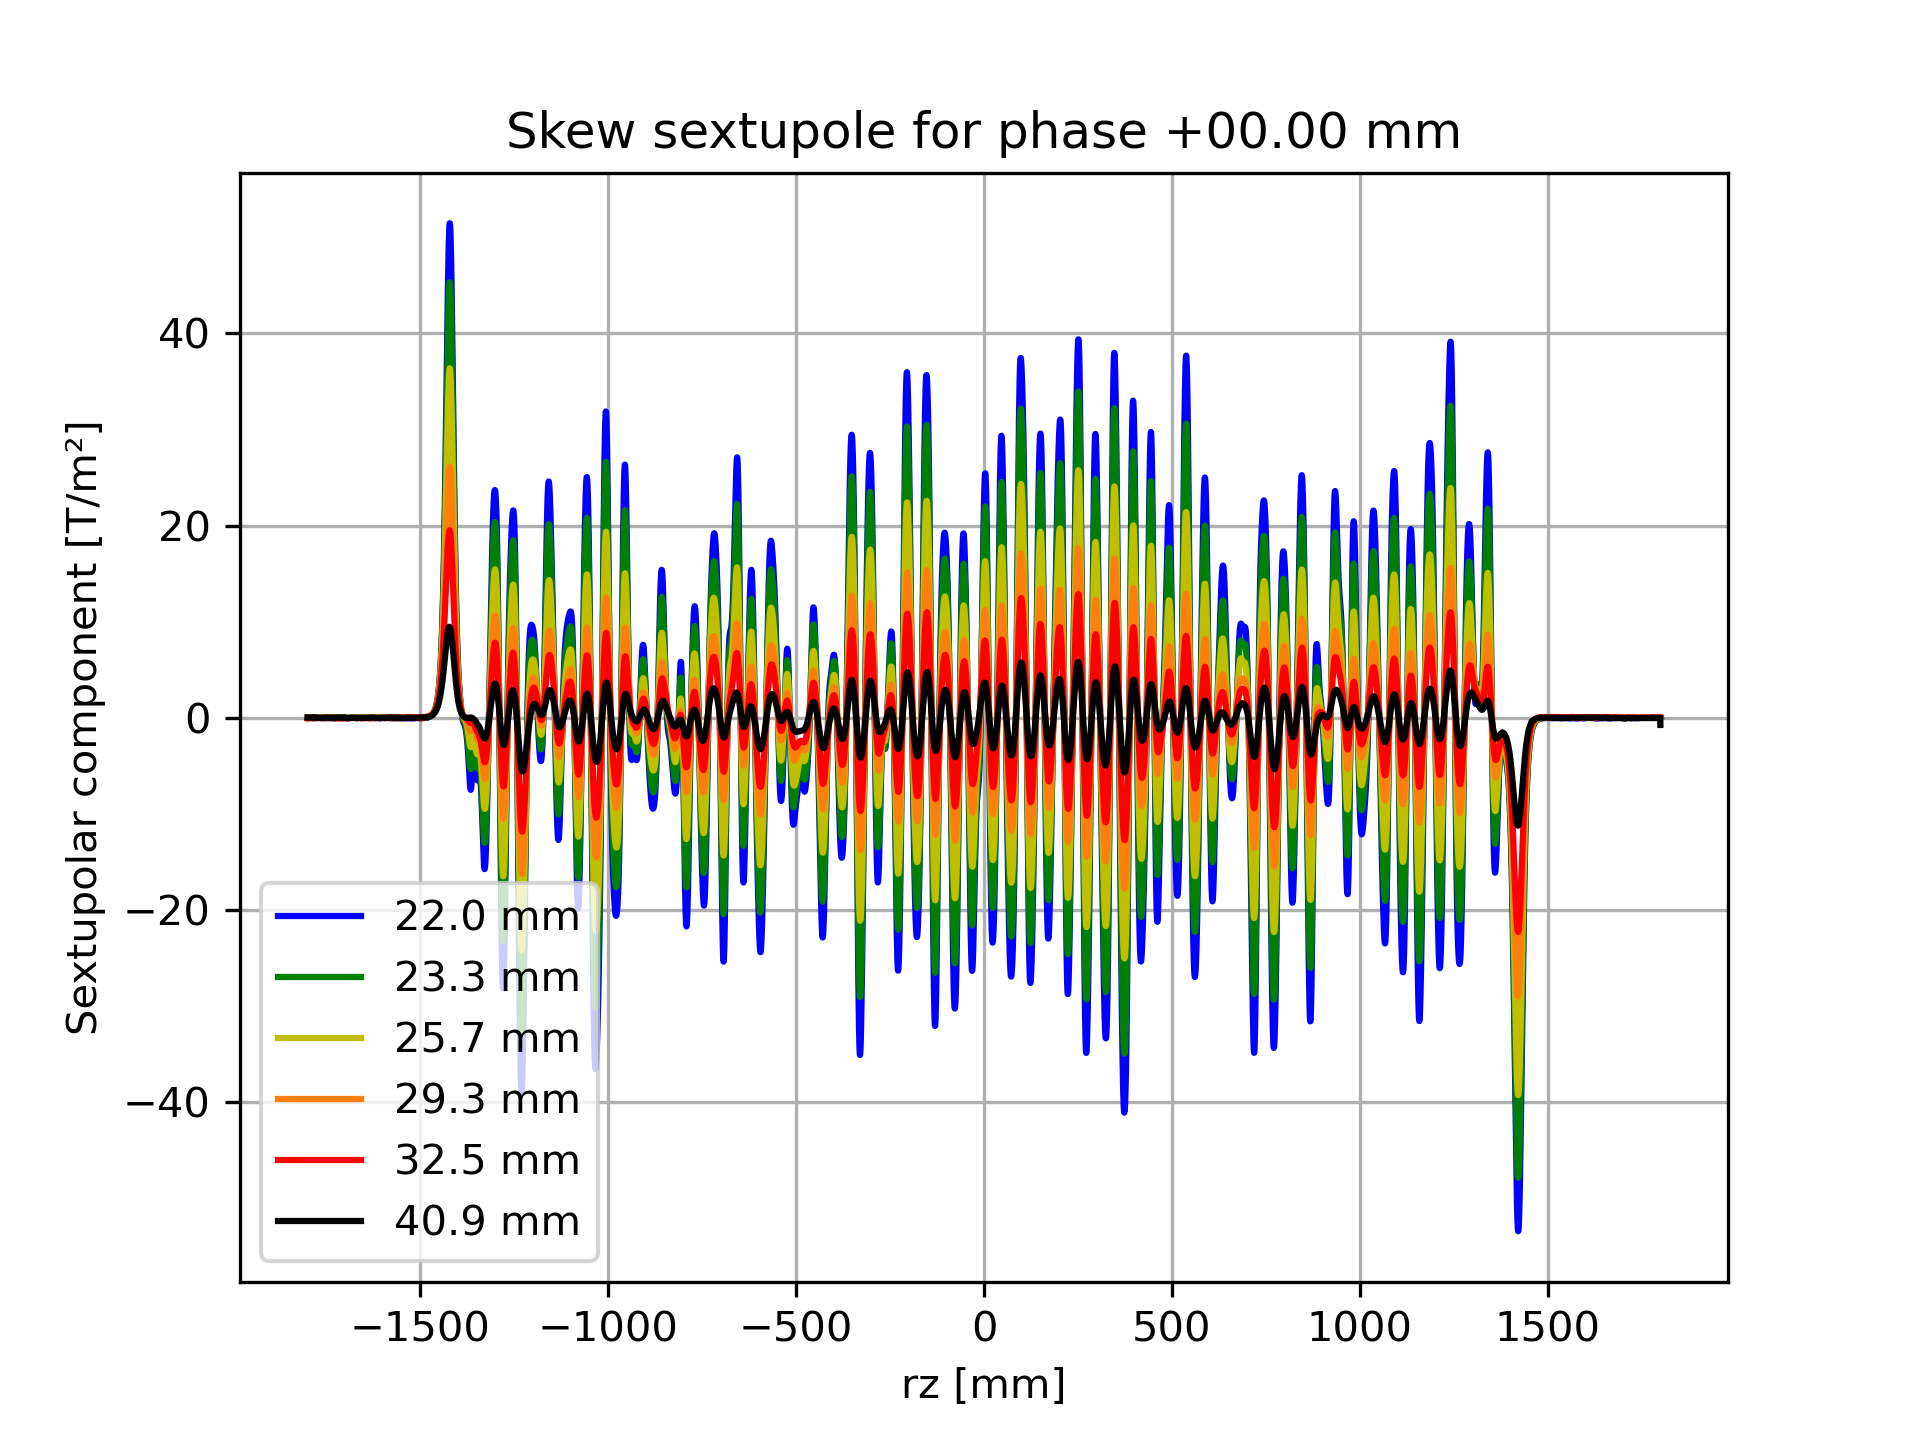
\includegraphics[width=0.9\linewidth, height=7cm]{figs/phase0 Skew sextupole.png}
\label{fig:subim20s}
\end{subfigure}
\caption{Componentes sextupolares de campo}
\label{fig:sext0}
\end{figure}

Os valores dos multipolos integrados para esta fase encontram-se detalhados na tabela abaixo.

\begin{table}[H]\footnotesize
\caption{Integrais das componentes multipolares}
\centering
\begin{tabular}{|c|c|c|c|c|}
\hline
   Gap [mm] &   Normal quadrupole [T] &   Skew quadrupole [T] &   Normal sextupole [T/m] &   Skew sextupole [T/m] \\
\hline
22.0 & +0.0265 & +0.0010 & +0.4712 & +0.3515 \\
23.3 & +0.0228 & +0.0006 & +0.3218 & +0.5067 \\
25.7 & +0.0178 & +0.0004 & +0.2881 & +0.3411 \\
29.3 & +0.0118 & -0.0004 & +0.2052 & +0.3045 \\
32.5 & +0.0078 & -0.0004 & +0.0920 & +0.2029 \\
40.9 & +0.0027 & -0.0011 & +0.2756 & +0.0263 \\
\hline
\end{tabular}
\end{table}



\subsection{Fase -16.39 mm}



\subsubsection{Campo vs gap}
\begin{figure}[H]
\hspace{4cm}
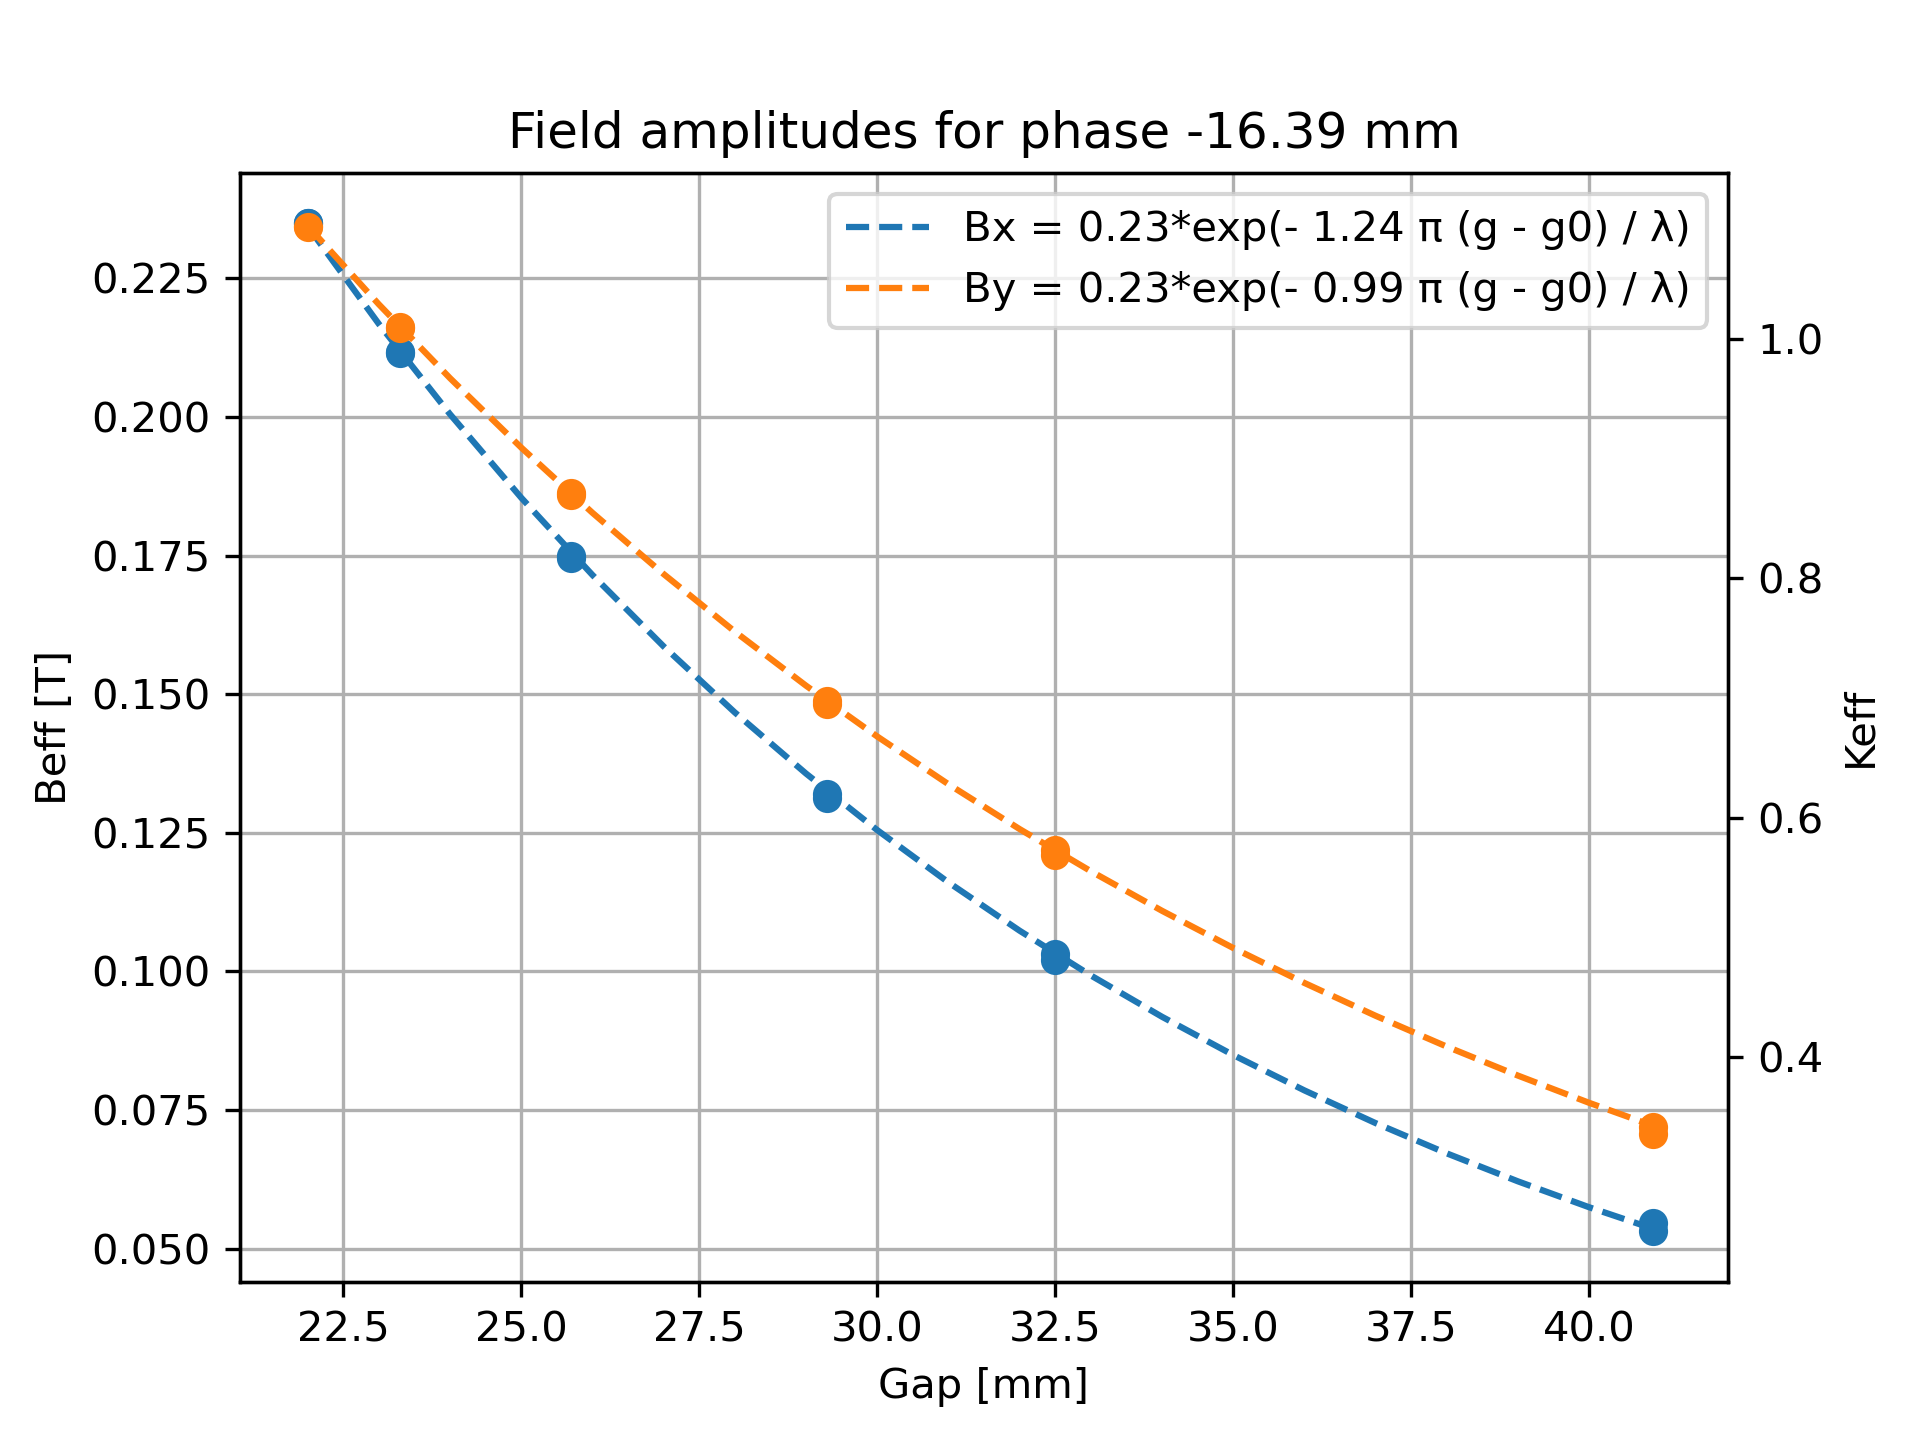
\includegraphics[width=0.5\textwidth]{figs/phase-16 B vs gap.png}
\caption{Beff vs gap fase = -16.39 mm}
\label{fig:fieldgap-16}
\end{figure}

\begin{table}[H]
\caption{Beff vs gap fase = -16.39 mm}
\centering
\begin{tabular}{|c|c|c|}
\hline
   Gap [mm] &   Bx [T] &   By [T] \\
\hline
       22.0   &     0.23 &     0.23 \\
       23.3 &     0.21 &     0.22 \\
       25.7 &     0.18 &     0.19 \\
       29.3 &     0.13 &     0.15 \\
       32.5 &    0.10 &    0.12 \\
       40.9 &     0.05 &     0.07 \\
\hline
\end{tabular}
\end{table}

\paragraph{} As figuras abaixo exibem os campos normalizados do ID na configuração em questão.



\begin{figure}[H]
\begin{subfigure}{0.5\textwidth}
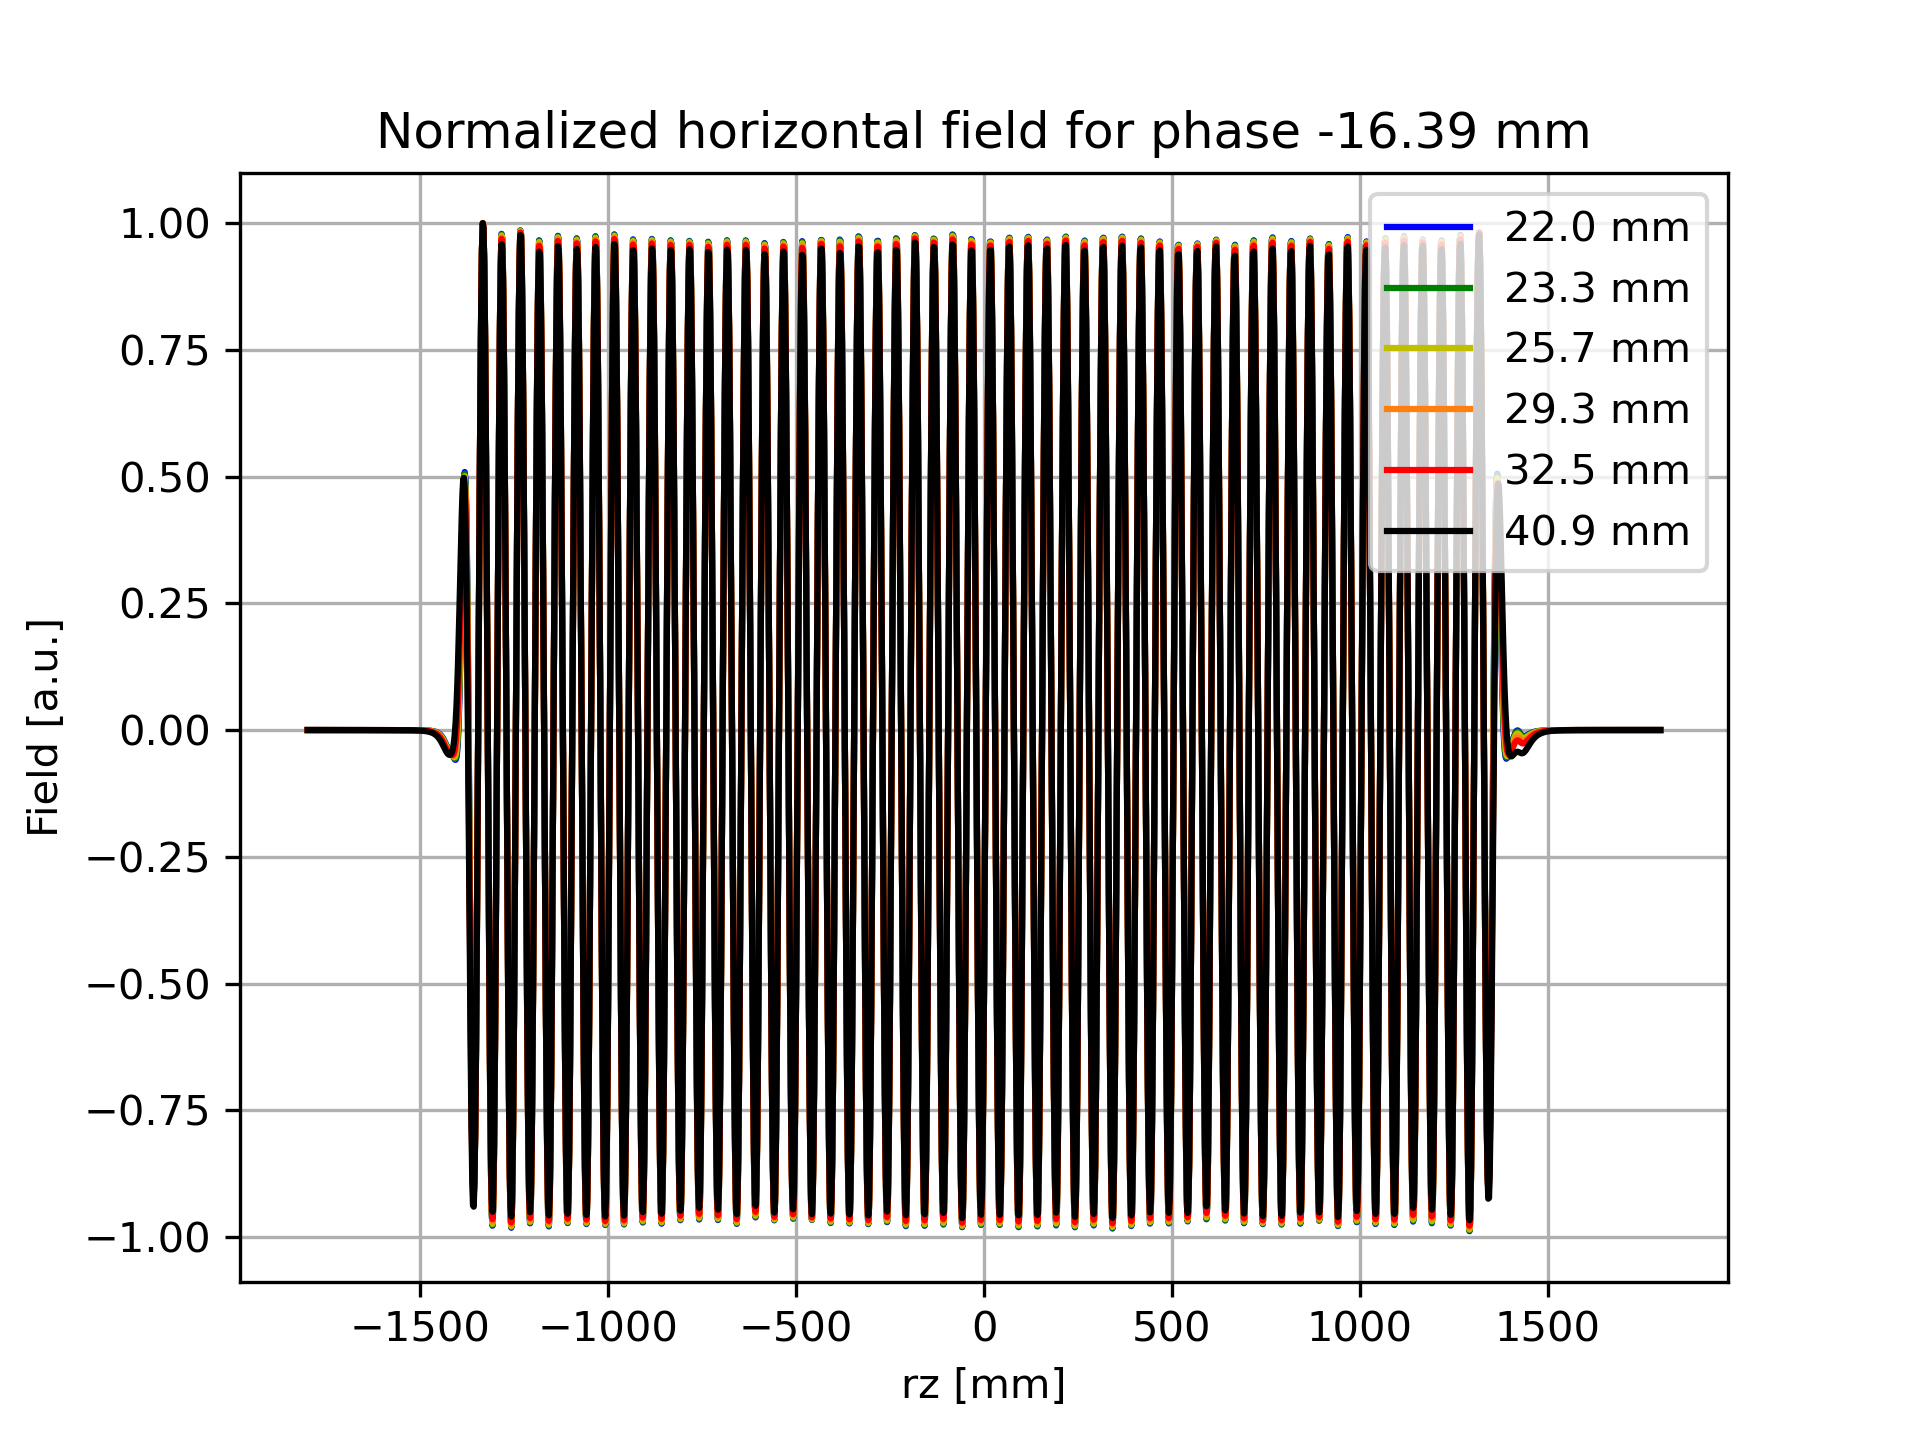
\includegraphics[width=0.9\linewidth, height=7cm]{figs/phase-16 Bx.png} 
\label{fig:subim1-16}
\end{subfigure}
\begin{subfigure}{0.5\textwidth}
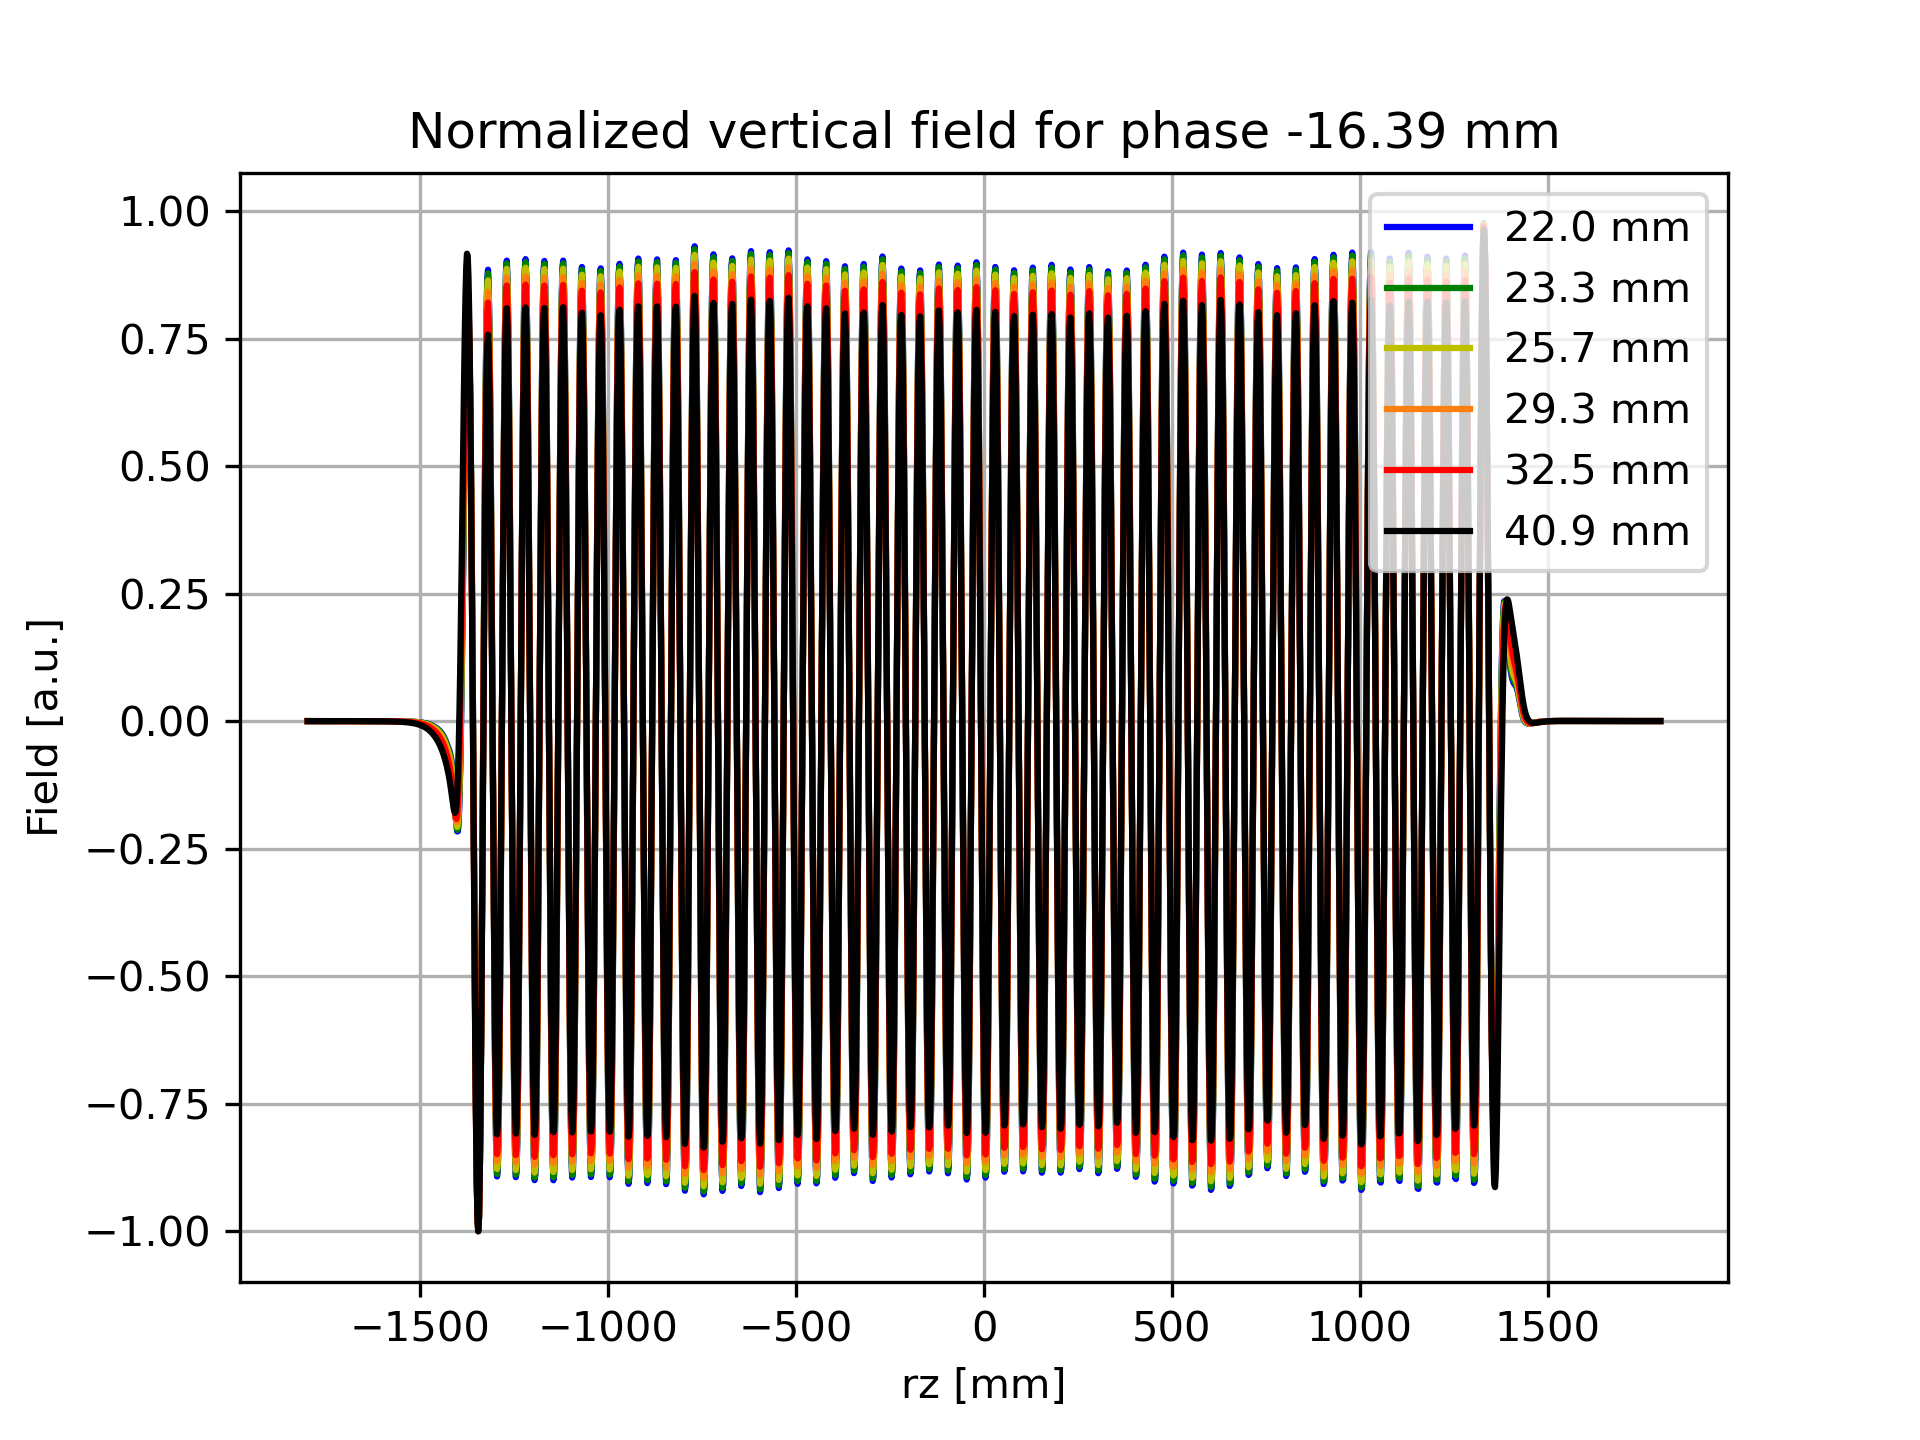
\includegraphics[width=0.9\linewidth, height=7cm]{figs/phase-16 By.png}
\label{fig:subim2-16}
\end{subfigure}
\caption{Componentes de campo horizontais (esquerda) e verticais (direita)}
\label{fig:bx_by-16}
\end{figure}

\begin{figure}[H]
\begin{center}
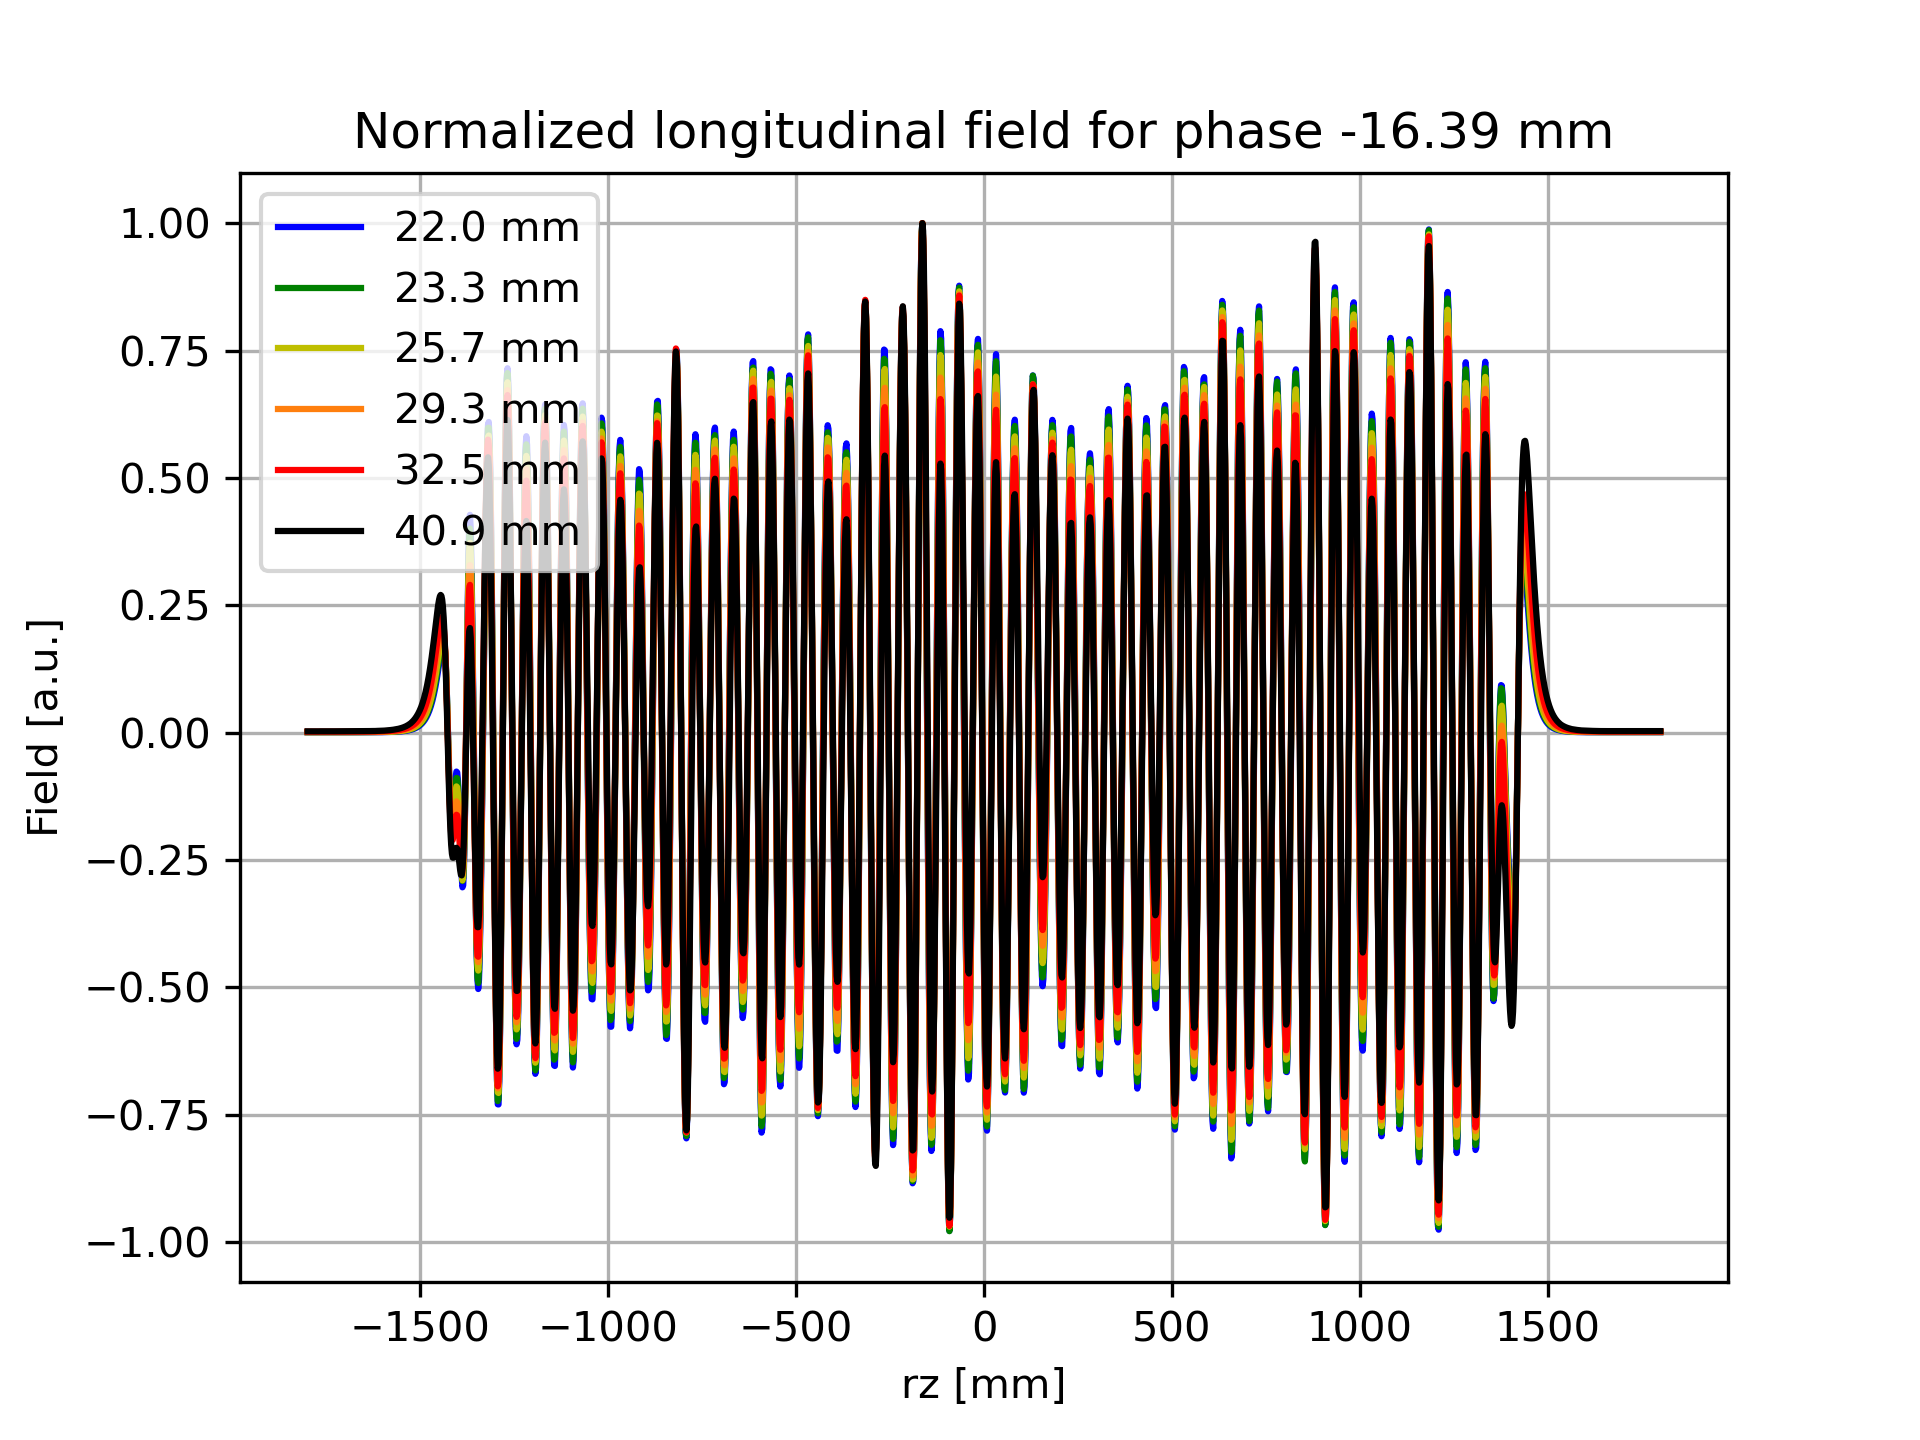
\includegraphics[width=0.5\textwidth]{figs/phase-16 Bz.png}
\caption{Componente longitudinal de campo normalizada}
\label{fig:bz-16}
\end{center}
\end{figure}

\subsubsection{Correções de órbita}

\begin{table}[H]
\centering
\caption{Tabela de correção local}
\begin{tabular}{|c|c|c|c|c|}
\hline
Gap {[}mm{]} & $\Delta$px up {[}$\mu$rad{]} & $\Delta$px down {[}$\mu$rad{]} & $\Delta$py up {[}$\mu$rad{]} & $\Delta$py down {[}$\mu$rad{]} \\ \hline
22.0 & 5.78  & -3.74 & 6.75 & 6.60 \\ \hline
23.3 & 5.11  & -4.03 & 7.79 & 5.99 \\ \hline
25.7 & 4.60  & -4.01 & 7.55 & 3.36 \\ \hline
29.3 & 3.29  & -4.27 & 8.45 & 1.30 \\ \hline
32.5 &  2.66 & -4.03 & 8.86 & -0.21 \\ \hline
40.9 & 0.90  & -3.68 & 9.15 & -2.75 \\ \hline
\end{tabular}
\label{tab:corff-16}
\end{table}

Os gráficos das figuras \ref{fig:-16corrx} e \ref{fig:-16corry} exibem a trajetória média após a correção com FOFB (gráficos da esquerda) e correções locais (gráficos da direita).

\begin{figure}[H]
\begin{subfigure}{0.5\textwidth}
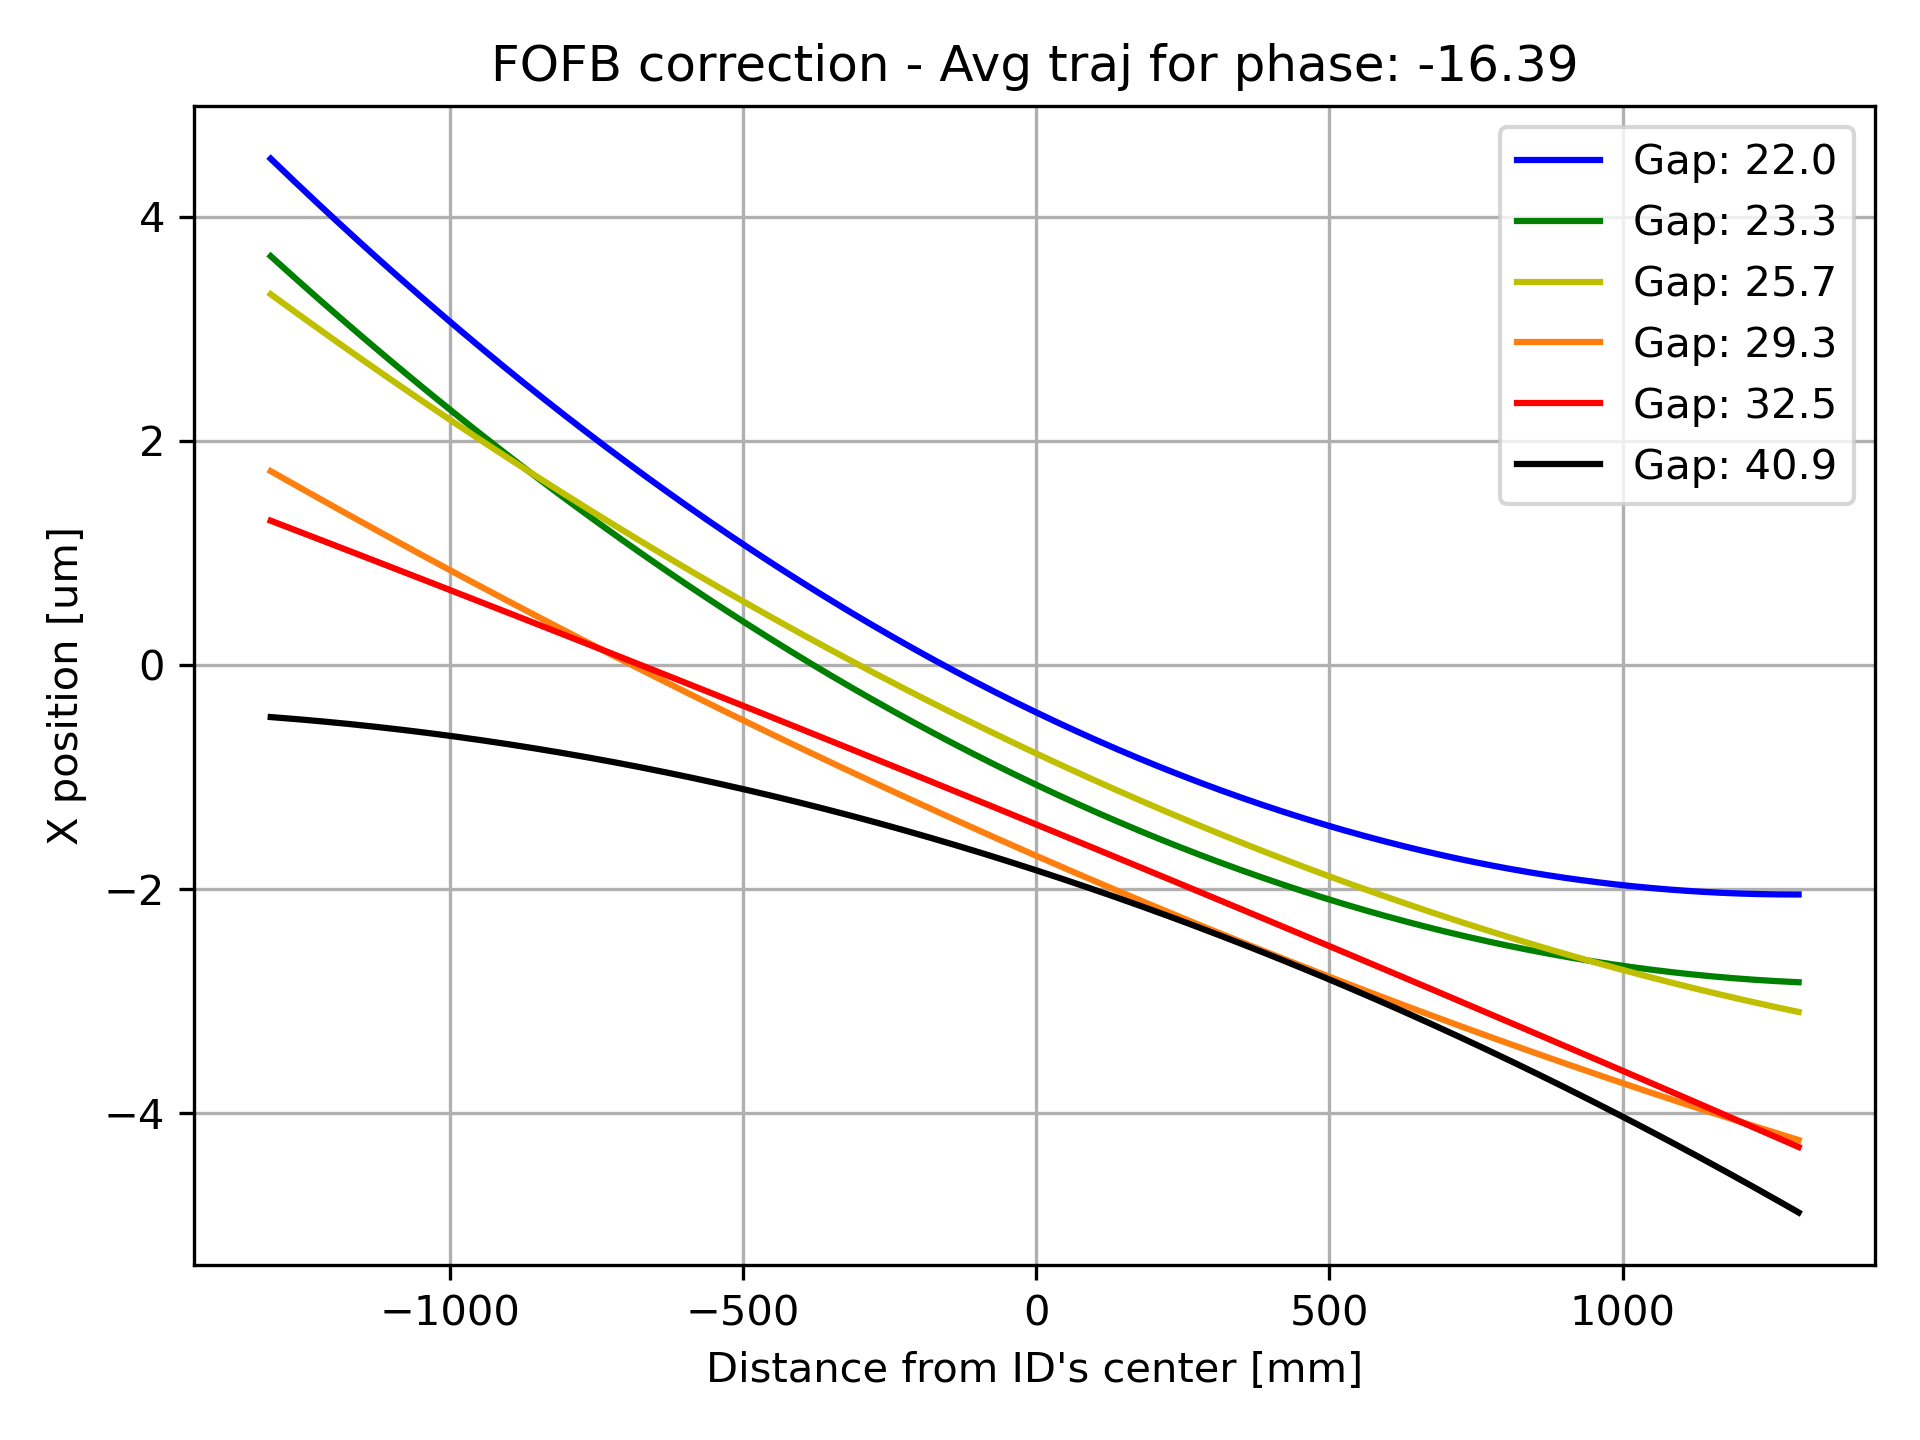
\includegraphics[width=0.9\linewidth, height=7cm]{figs/phase-16 horizontal-avg-traj-FOFB.png} 
\label{fig:subim10xc-16}
\end{subfigure}
\begin{subfigure}{0.5\textwidth}
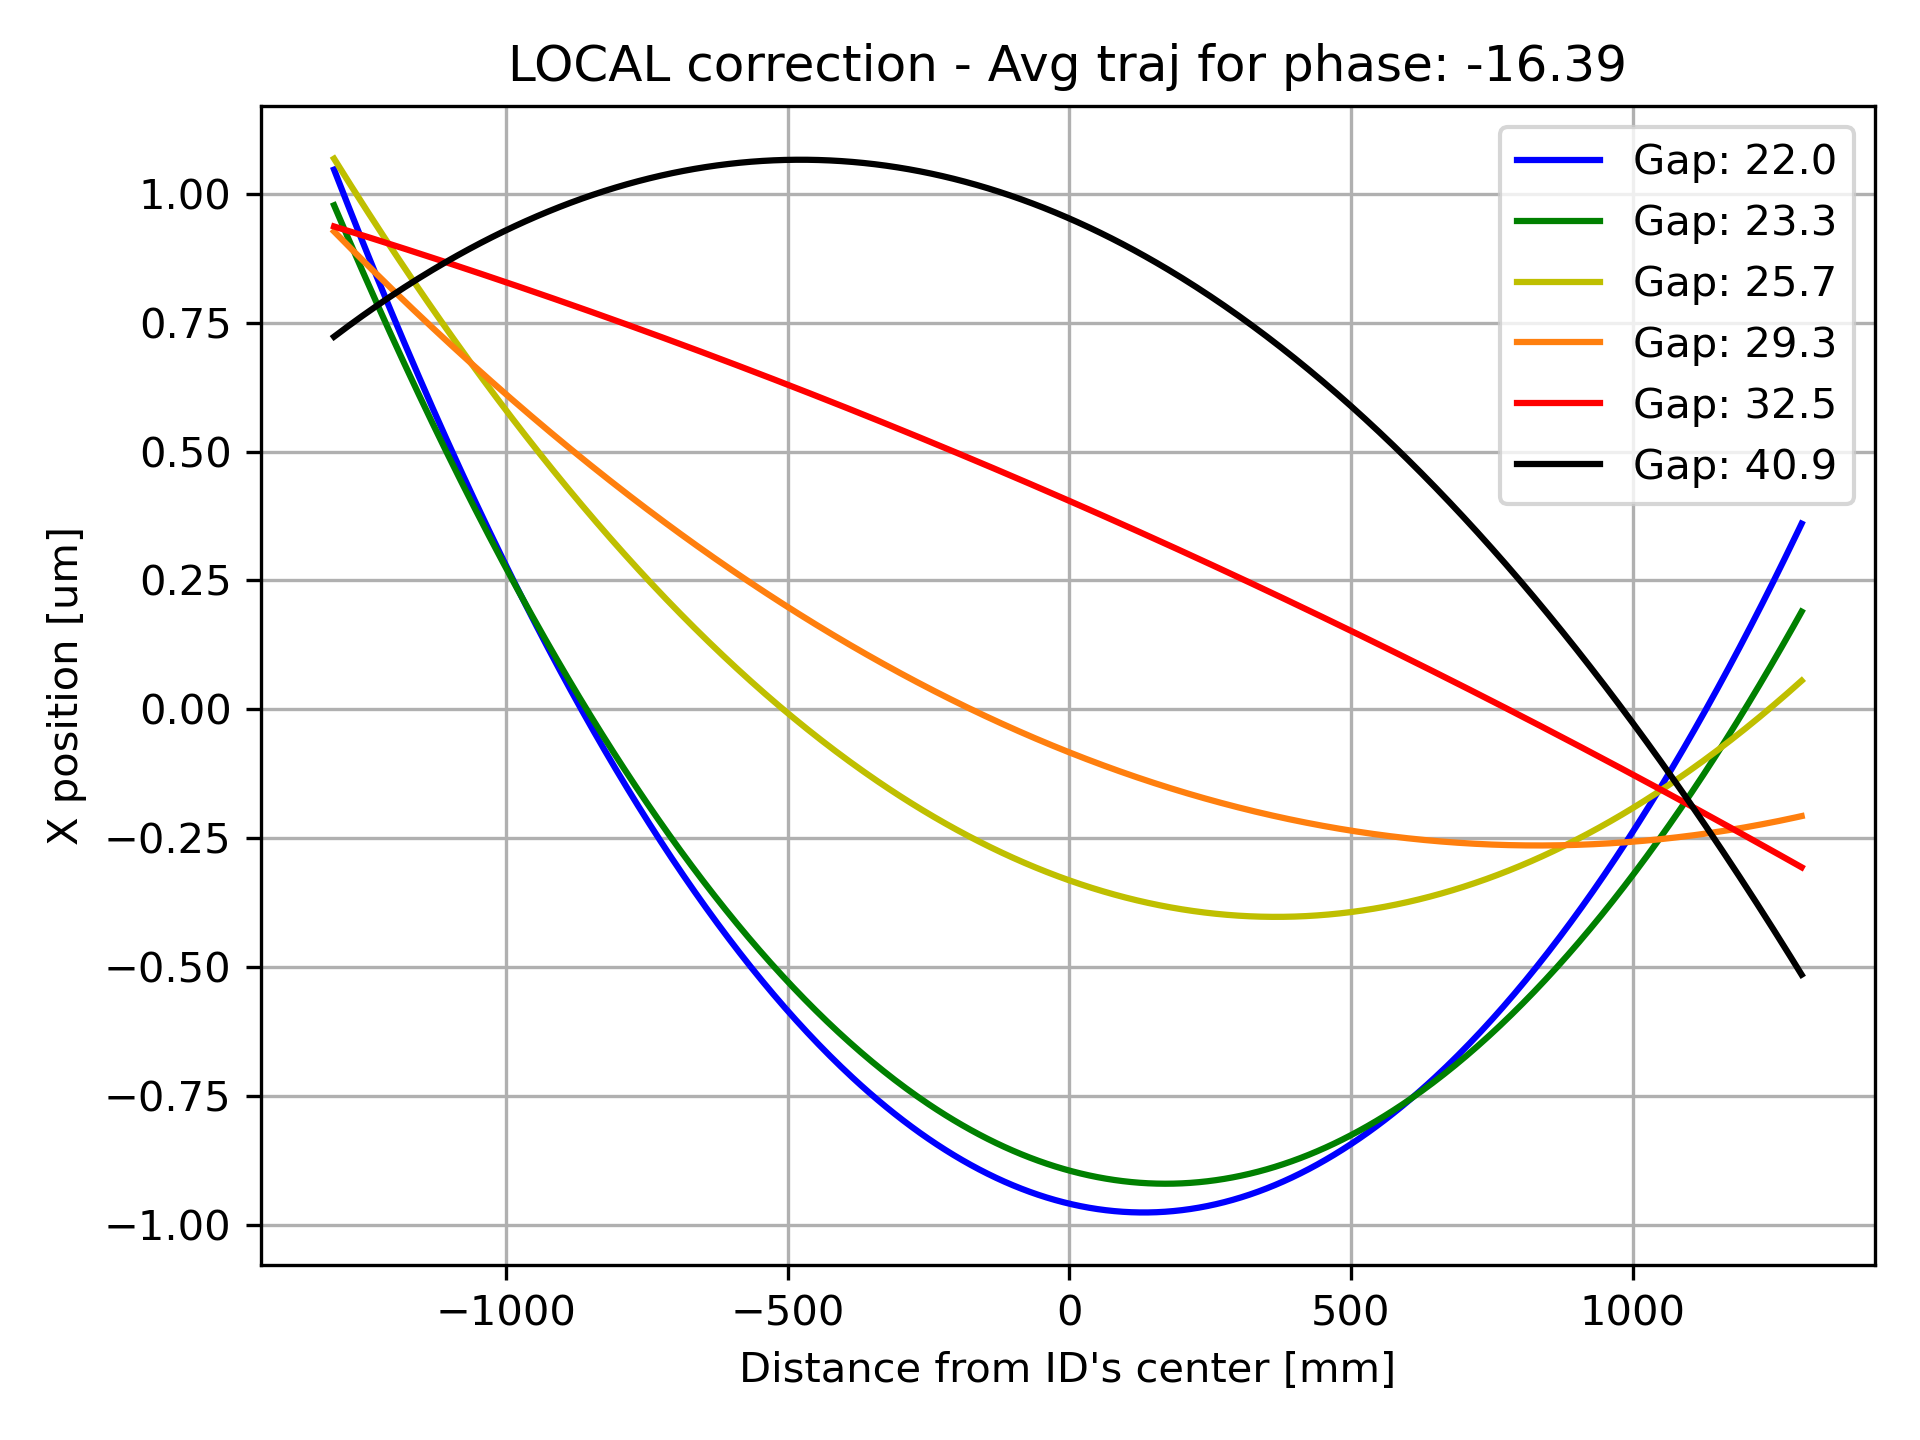
\includegraphics[width=0.9\linewidth, height=7cm]{figs/phase-16 horizontal-avg-traj-LOCAL.png}
\label{fig:subim20xc-16}
\end{subfigure}
\caption{Trajetória média horizontal após correções de órbita utilizando FOFB (esquerda) e feedforward (direita)}
\label{fig:-16corrx}
\end{figure}

\begin{figure}[H]
\begin{subfigure}{0.5\textwidth}
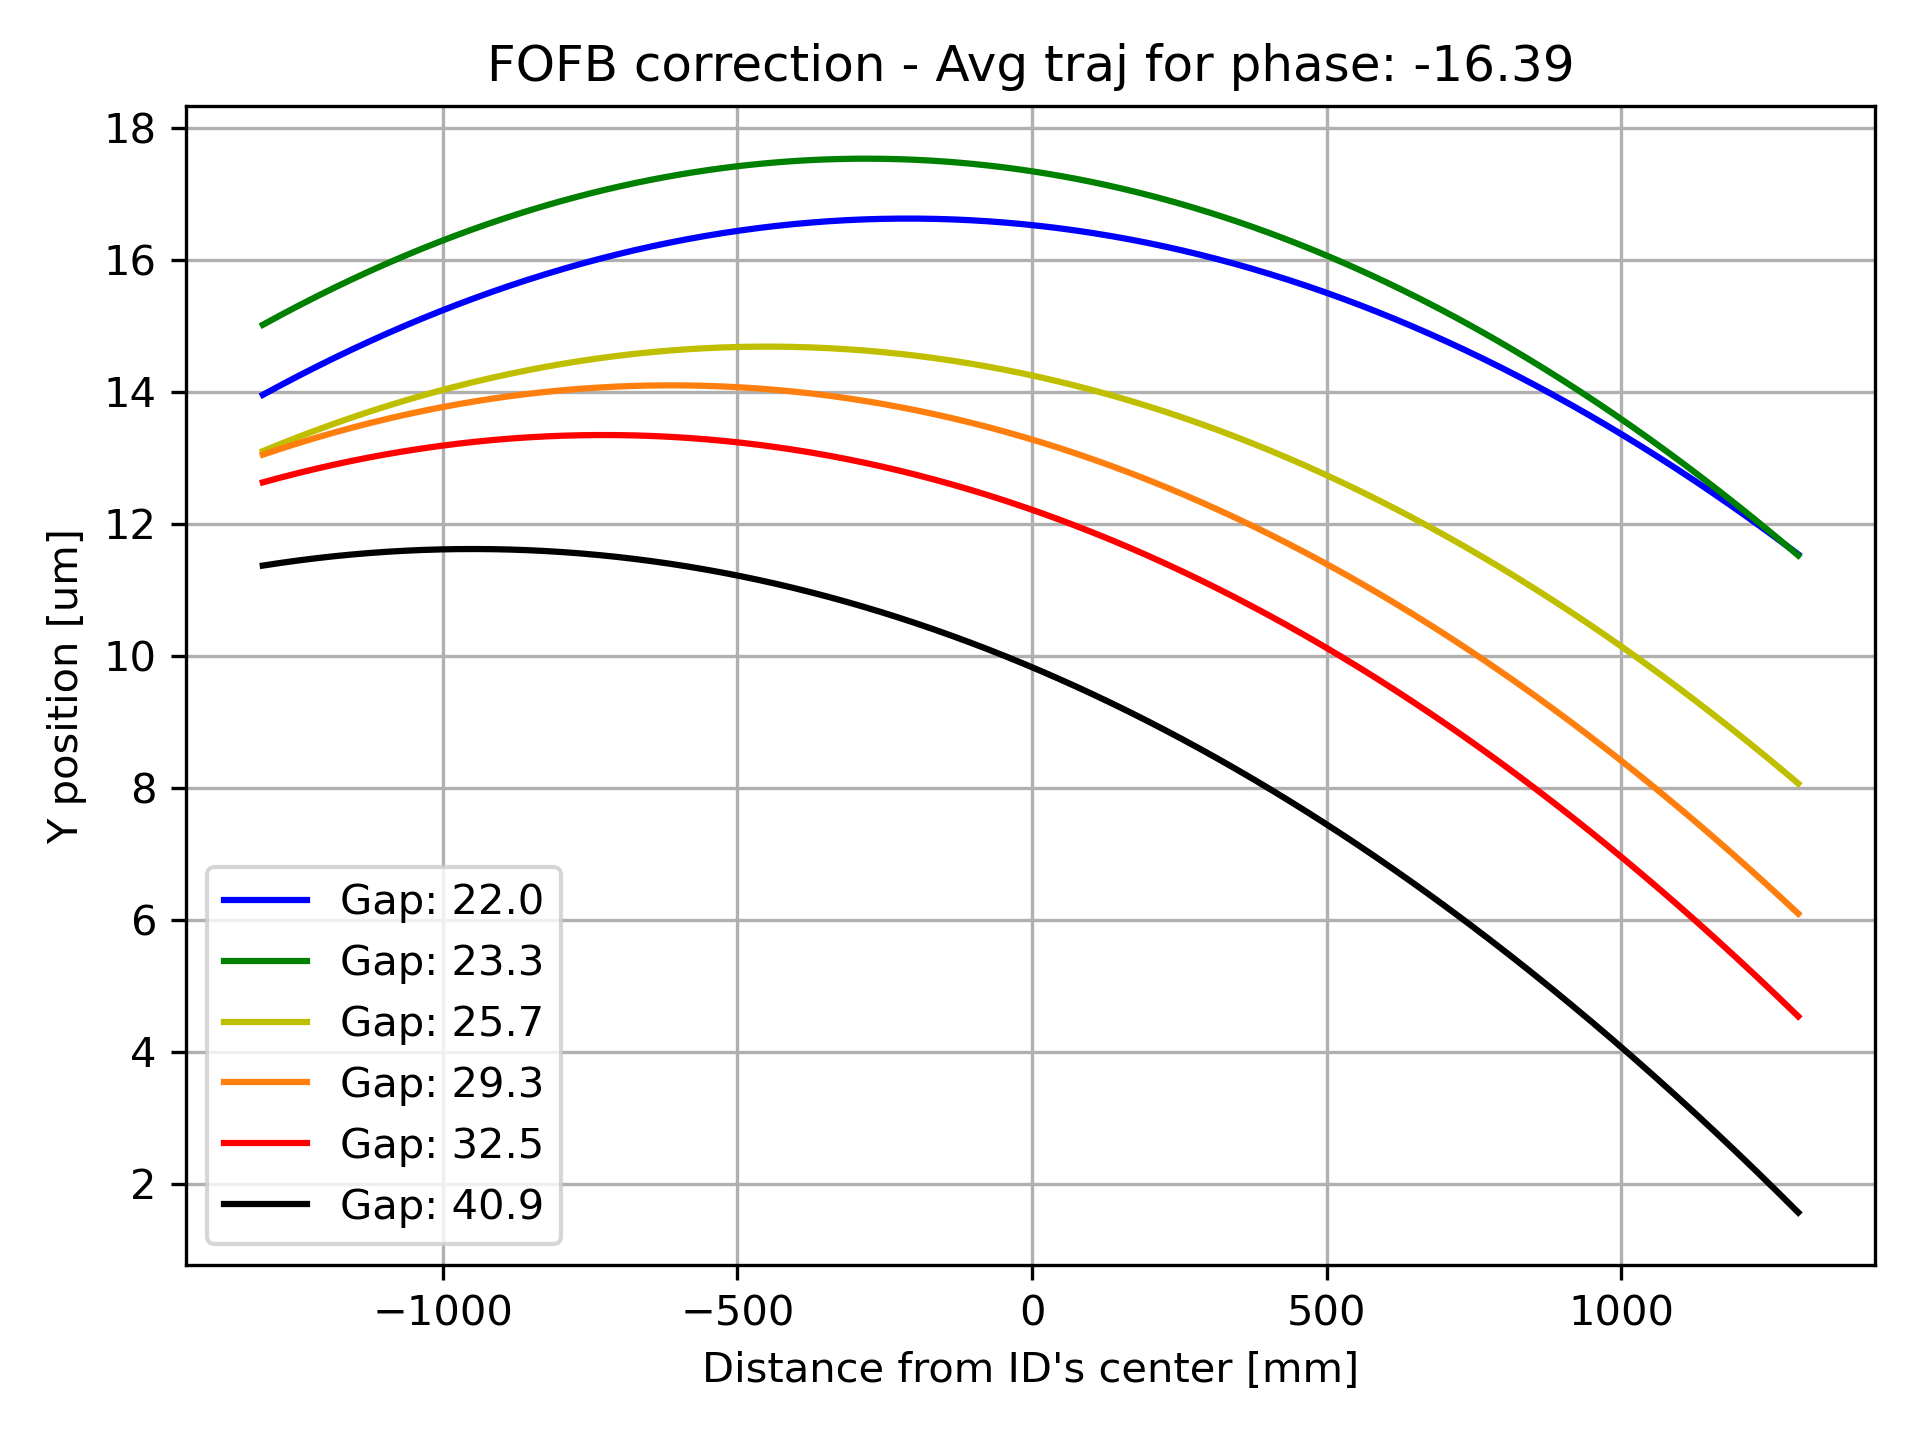
\includegraphics[width=0.9\linewidth, height=7cm]{figs/phase-16 vertical-avg-traj-FOFB.png} 
\label{fig:subim10yc-16}
\end{subfigure}
\begin{subfigure}{0.5\textwidth}
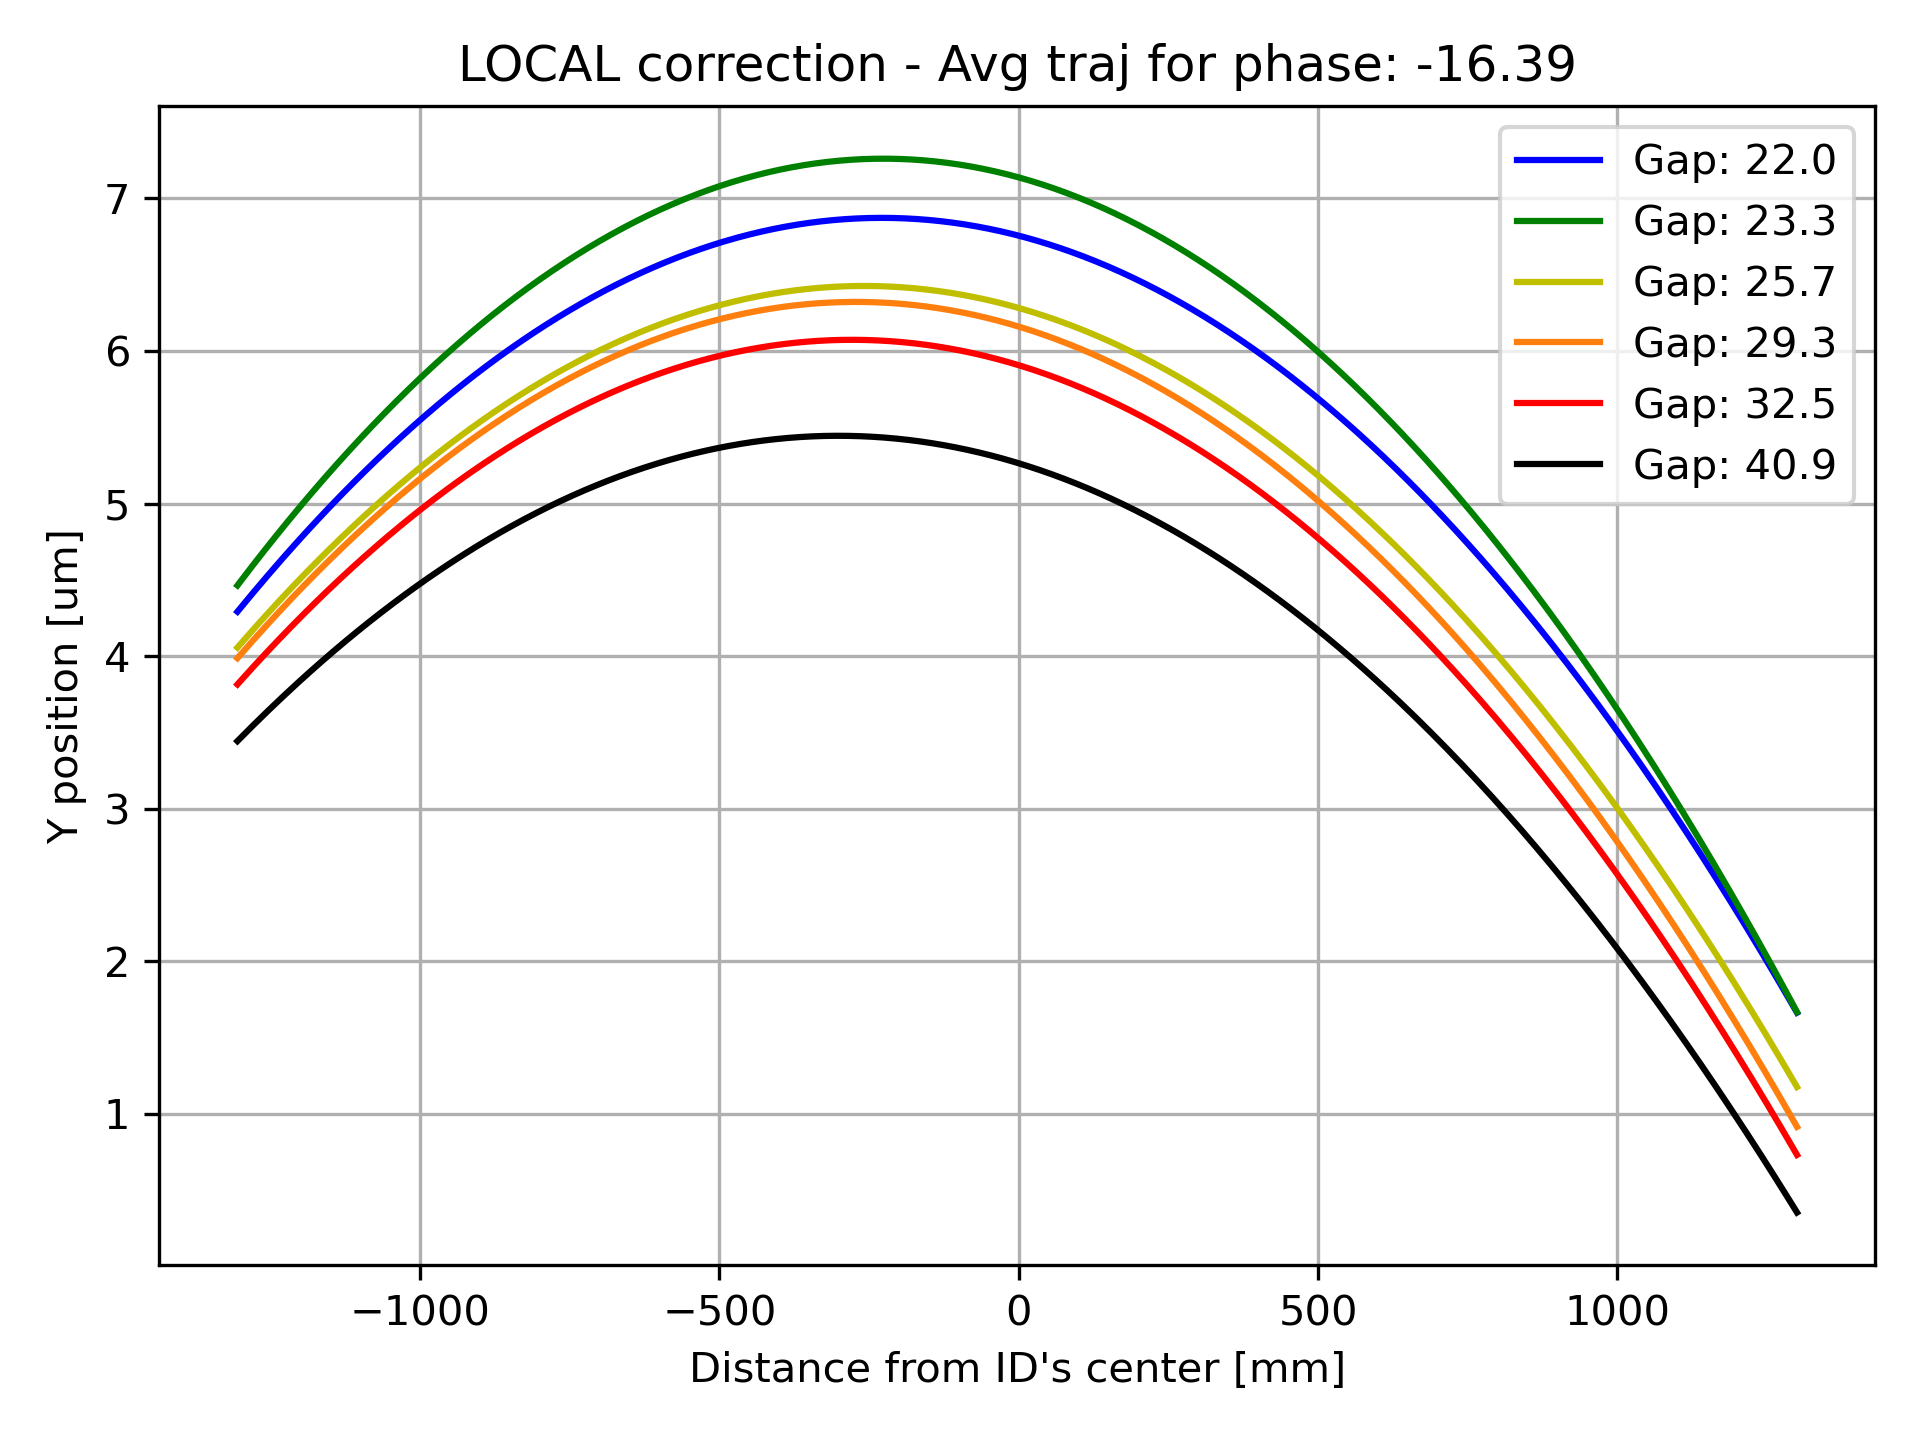
\includegraphics[width=0.9\linewidth, height=7cm]{figs/phase-16 vertical-avg-traj-LOCAL.png}
\label{fig:subim20yc-16}
\end{subfigure}
\caption{Trajetória média vertical após correções de órbita utilizando FOFB (esquerda) e feedforward (direita)}
\label{fig:-16corry}
\end{figure}



\subsubsection{Trajetória}


\begin{figure}[H]
\begin{subfigure}{0.5\textwidth}
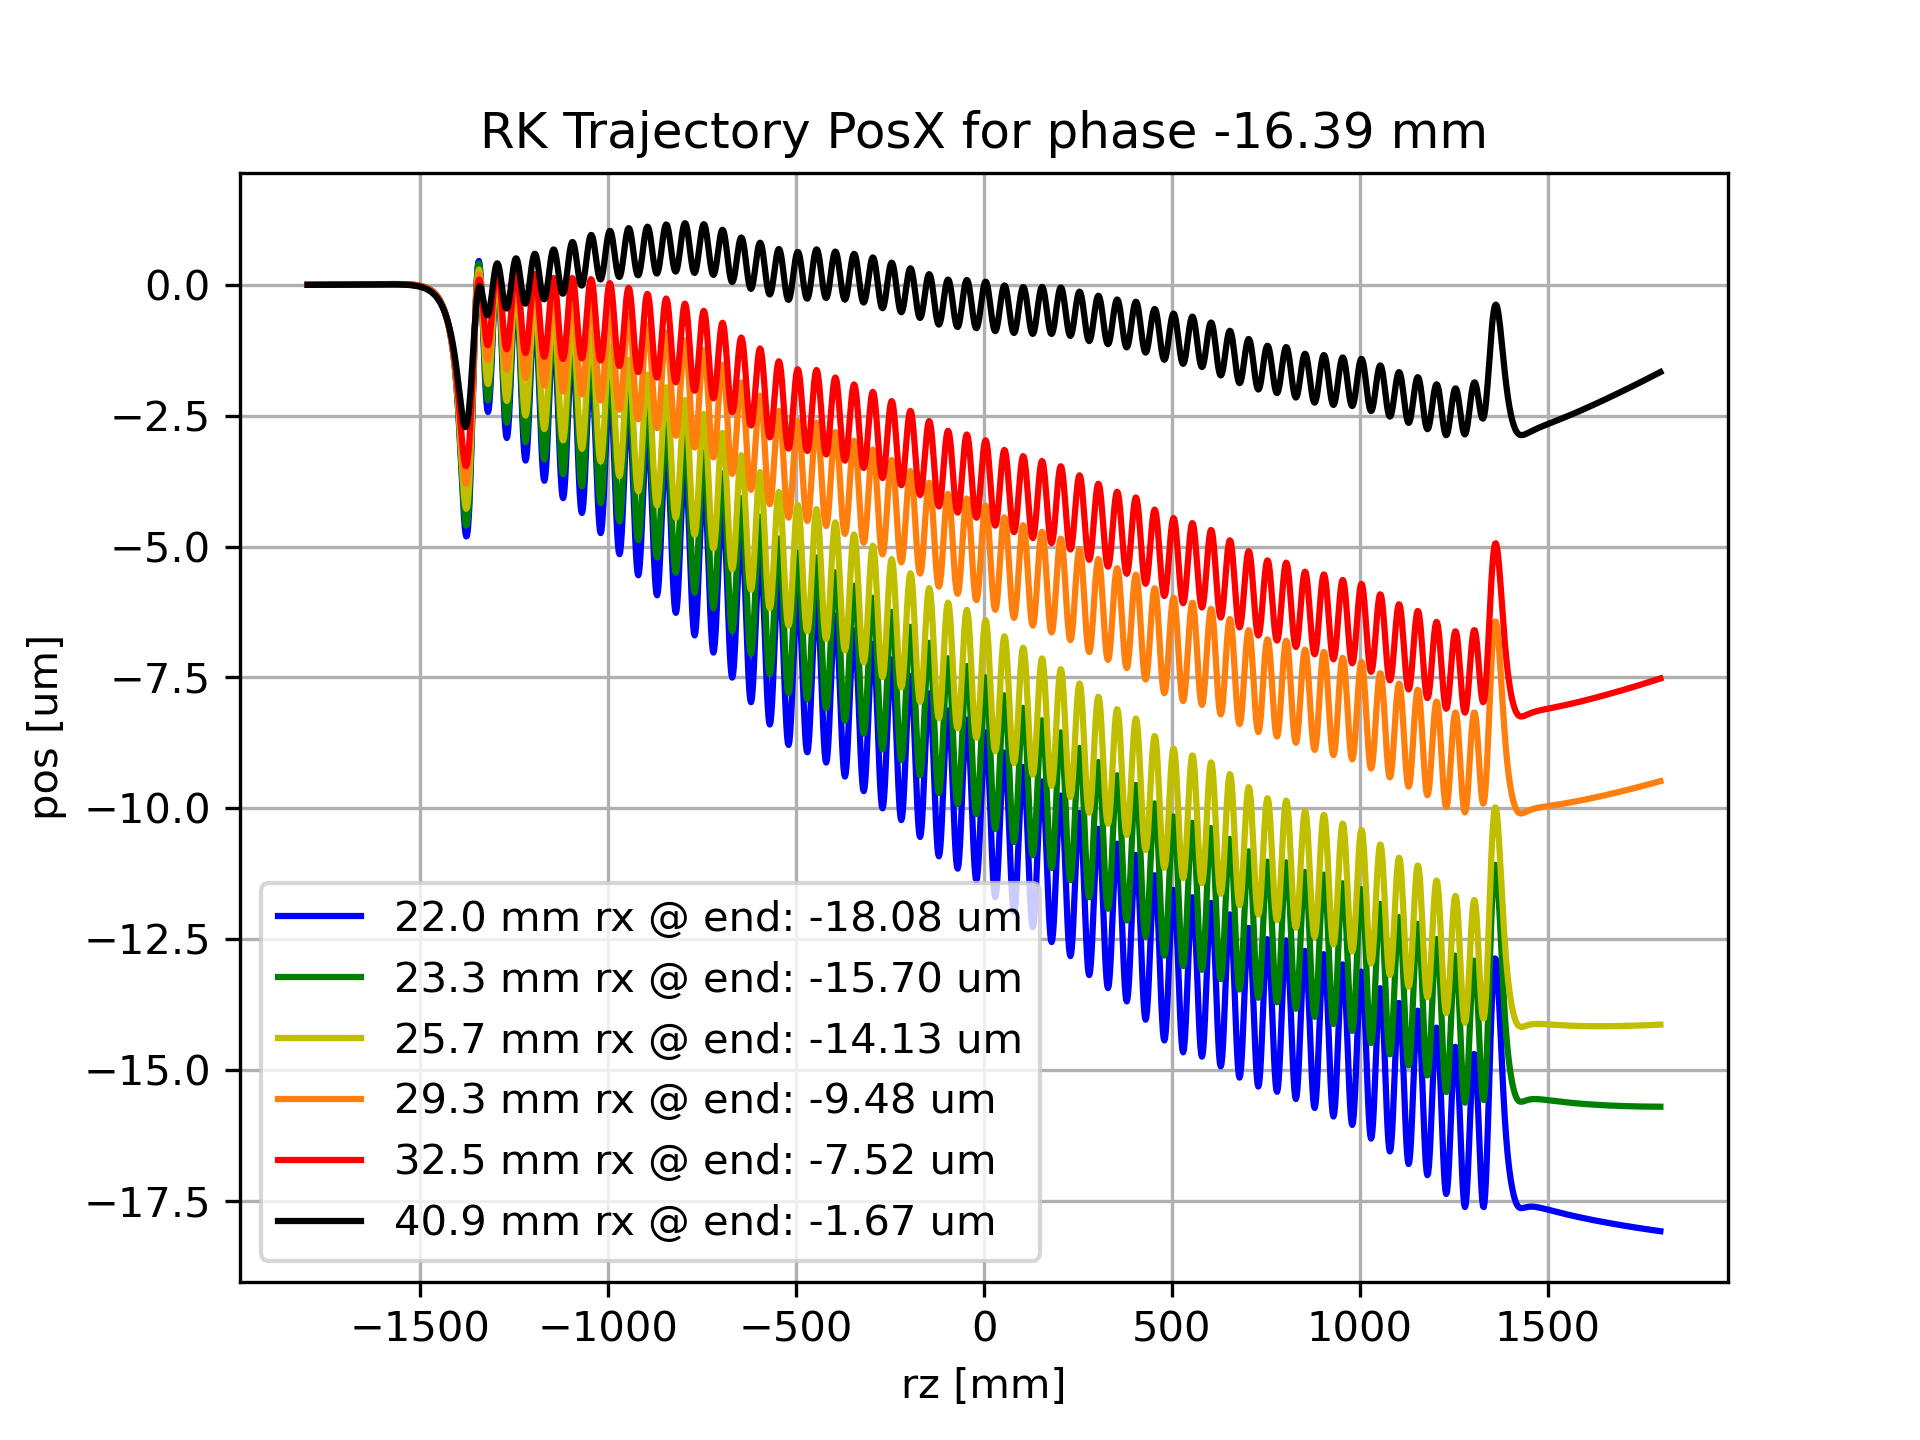
\includegraphics[width=0.9\linewidth, height=7cm]{figs/phase-16 RK Posx.png} 
\label{fig:subim1-16tx}
\end{subfigure}
\begin{subfigure}{0.5\textwidth}
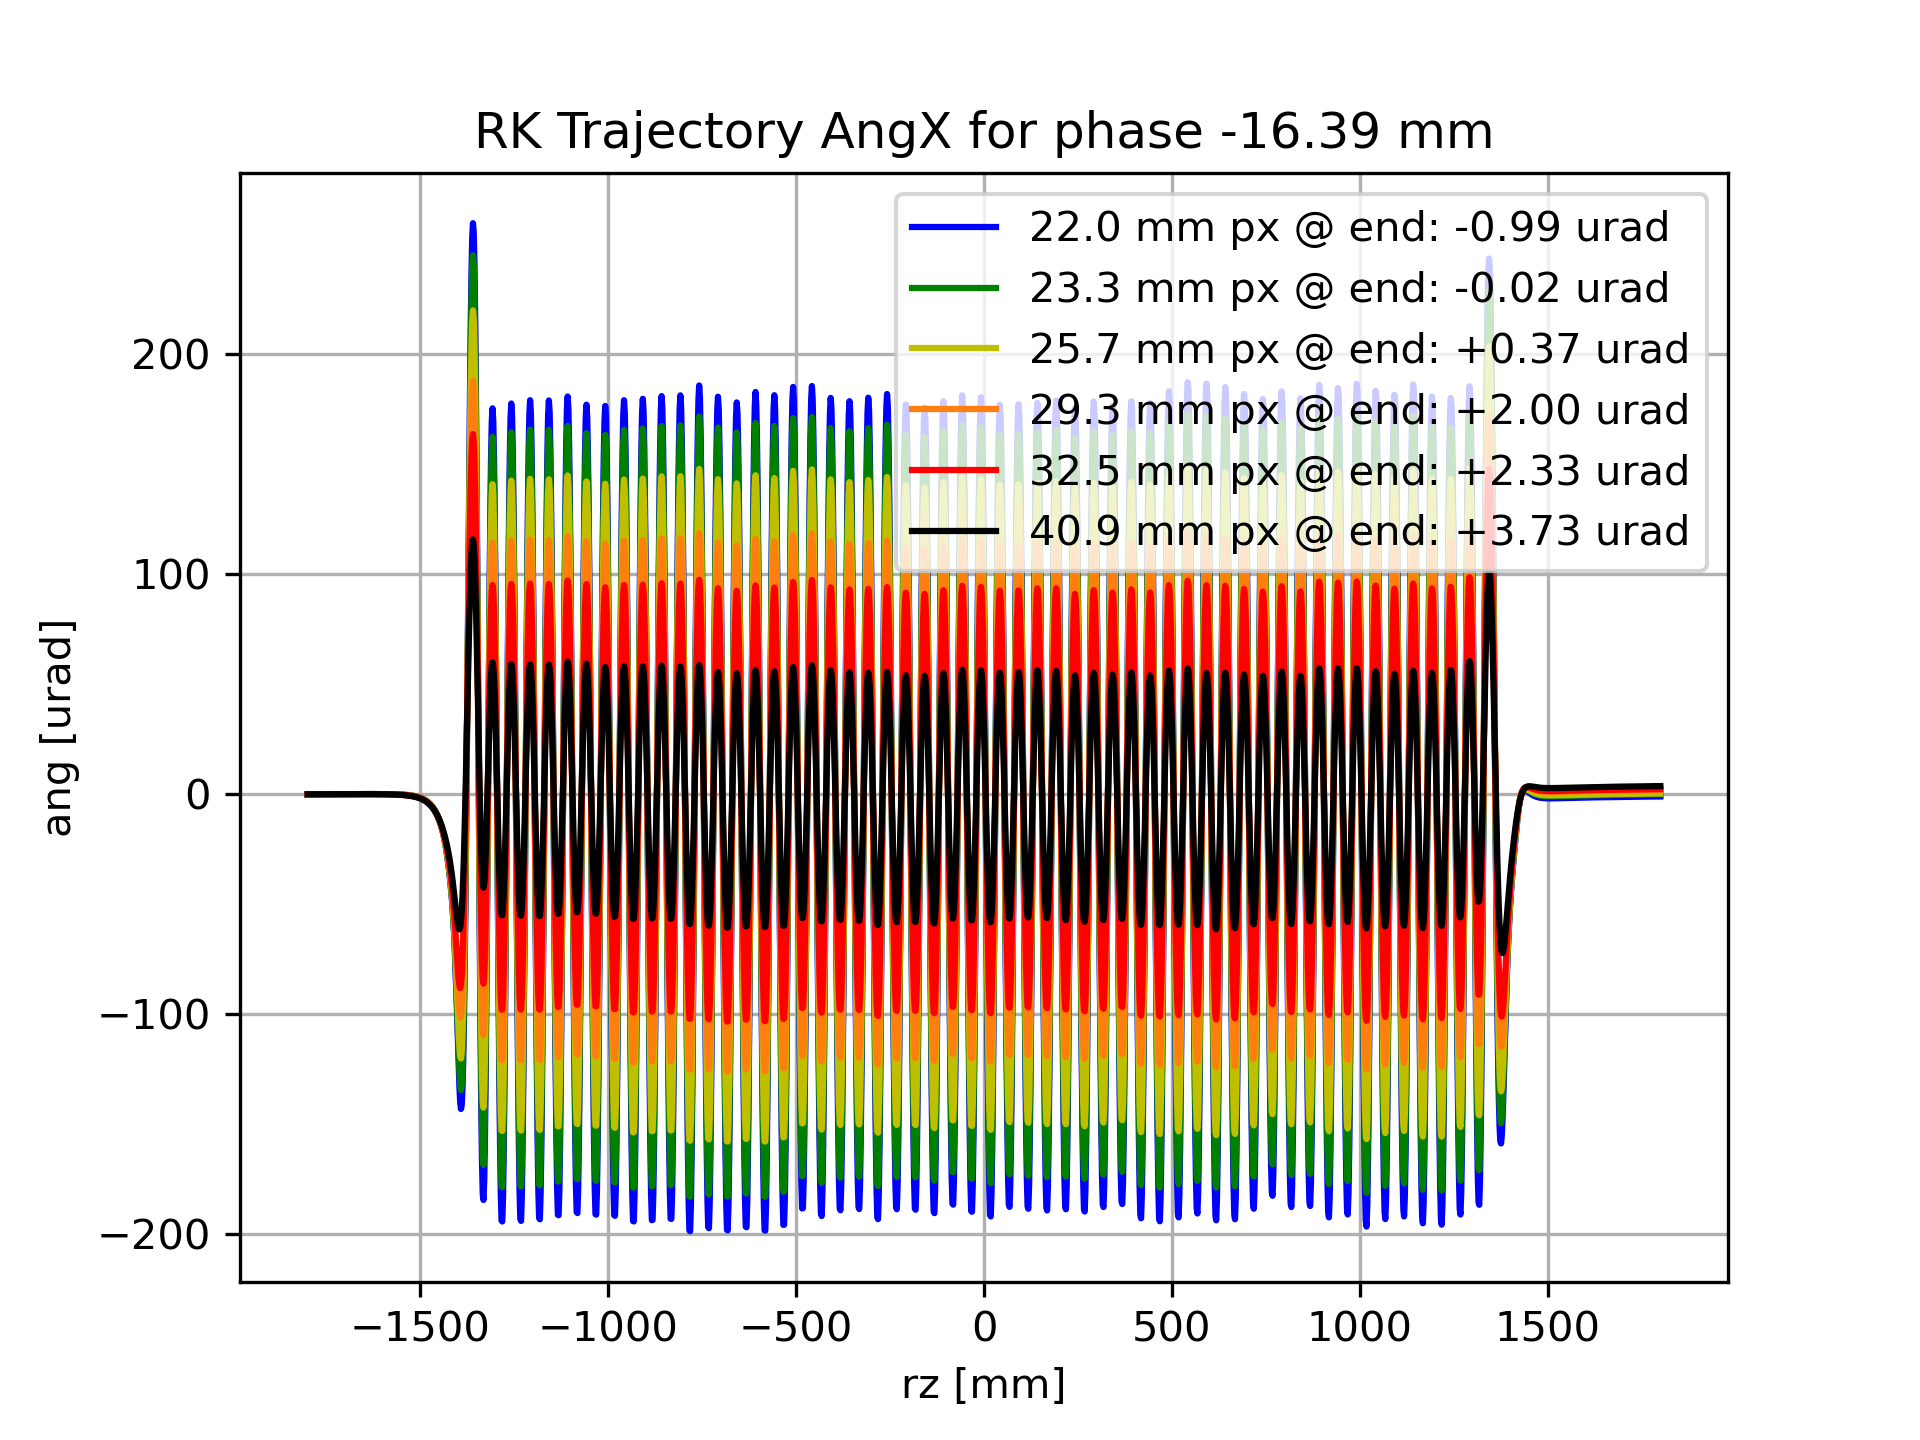
\includegraphics[width=0.9\linewidth, height=7cm]{figs/phase-16 RK Angx.png}
\label{fig:subim2-16tx}
\end{subfigure}
\caption{Trajetória X para fase -16.39 mm}
\label{fig:trajx-16}
\end{figure}

\begin{figure}[H]
\begin{subfigure}{0.5\textwidth}
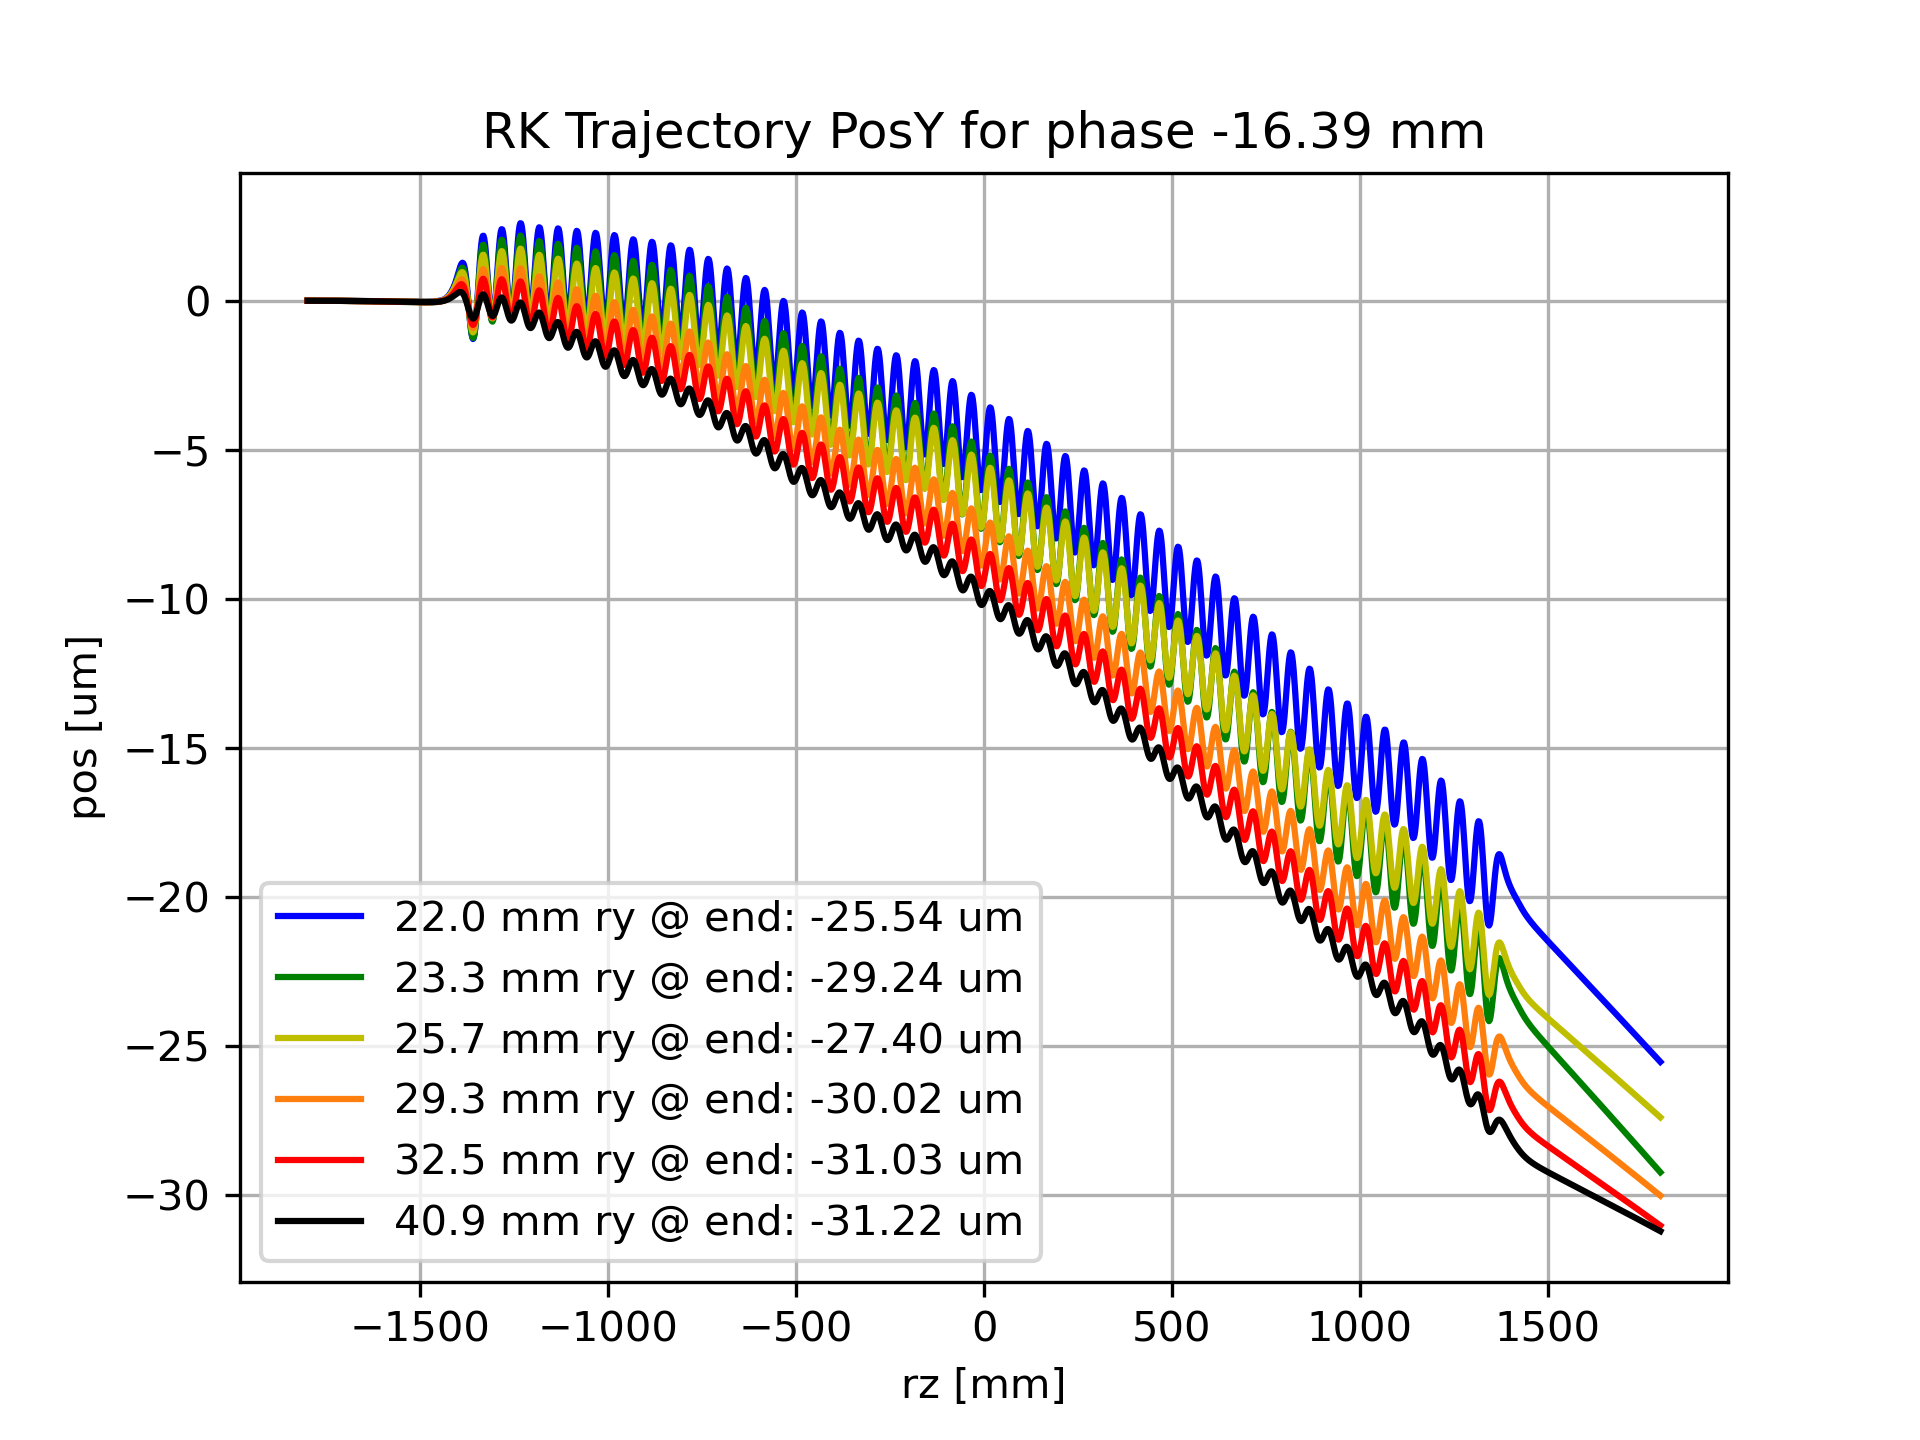
\includegraphics[width=0.9\linewidth, height=7cm]{figs/phase-16 RK Posy.png} 
\label{fig:subim1-16ty}
\end{subfigure}
\begin{subfigure}{0.5\textwidth}
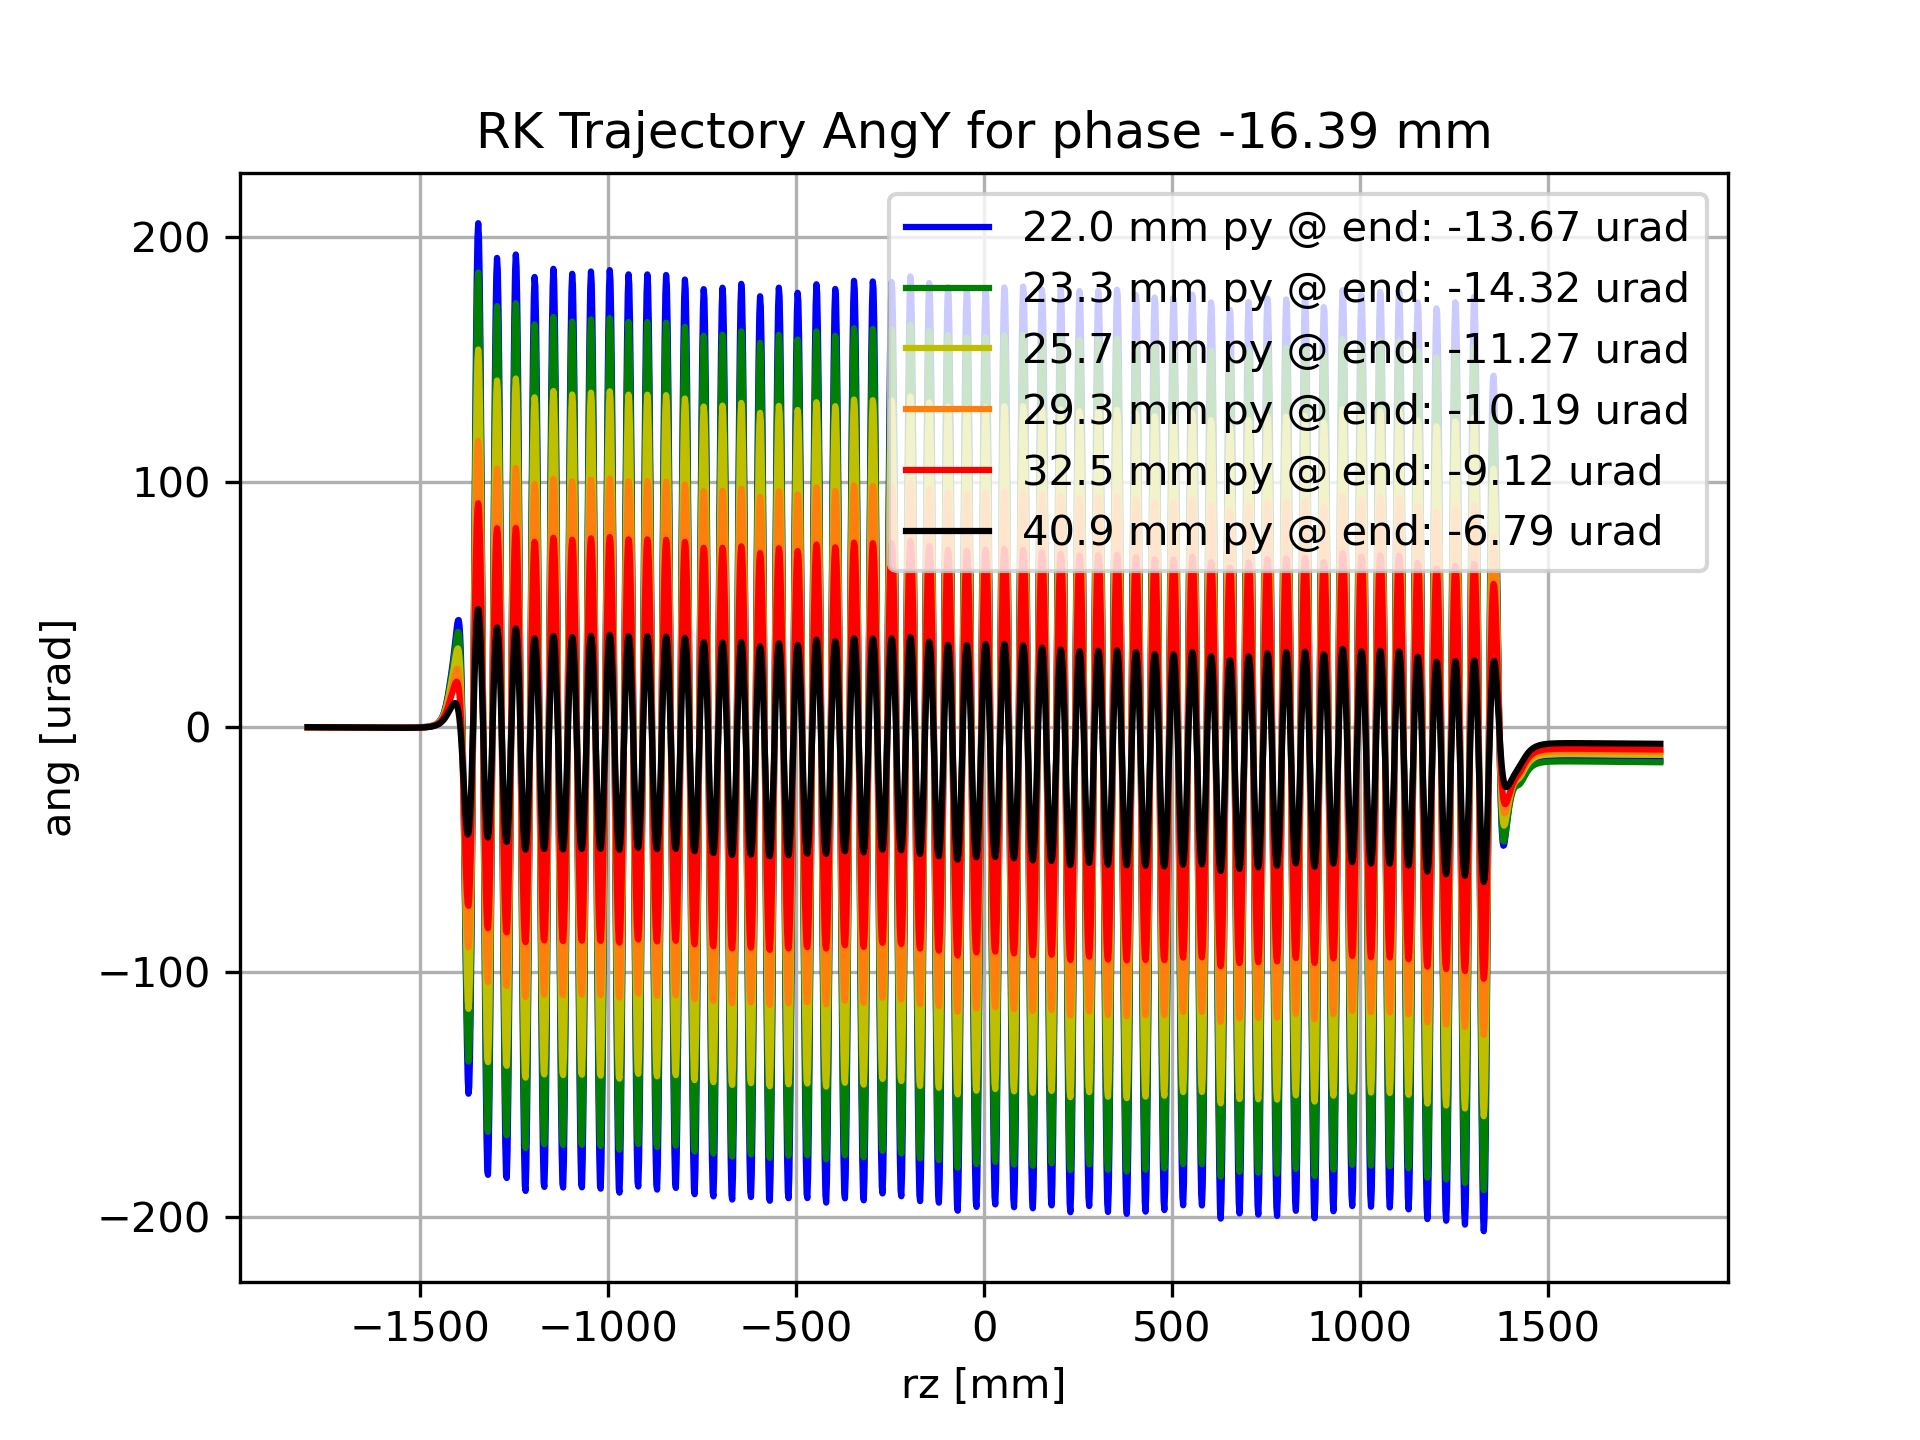
\includegraphics[width=0.9\linewidth, height=7cm]{figs/phase-16 RK Angy.png}
\label{fig:subim2-16ty}
\end{subfigure}
\caption{Trajetória Y para fase -16.39 mm}
\label{fig:trajy-16}
\end{figure}

Os valores finais de ângulo e trajetória mostrados nas figuras acima estão resumidos nas tabelas abaixo, em conjunto com as integrais de campo.


\begin{table}[H]
\centering
\caption{Primeiras integrais de campo}
\begin{tabular}{|c|c|c|}
\hline
   Gap [mm] & Bx 1st integral [G cm] / $\Delta$ py [$\mu$rad] & By 1st integral [G cm] / $\Delta$ px [$\mu$rad] \\
\hline
    22.0 & +138.0 / -13.67 & -13.2 / -0.99 \\
    23.3 & +144.2 / -14.32 &  -2.8 / -0.02 \\
    25.7 & +113.5 / -11.27 &  +1.9 / +0.37 \\
    29.3 & +102.4 / -10.19 & +19.0 / +2.00 \\
    32.5 & +91.5 / -9.12 & +22.7 / +2.33 \\
    40.9 & +68.0 / -6.79 & +37.1 / +3.73 \\
\hline
\end{tabular}
\end{table}

\begin{table}[H]
\centering
\caption{Segundas integrais de campo}
\begin{tabular}{|c|c|c|}
\hline
   Gap [mm] & Bx 2nd integral [G cm²] / $\Delta$ y [$\mu$m] & By 2nd integral [G cm²] / $\Delta$ x [$\mu$m]   \\
\hline
    22.0 & +2.58e+04 / -25.54 & -1.86e+04 / -18.08 \\
    23.3 & +2.94e+04 / -29.24 & -1.61e+04 / -15.70 \\
    25.7 & +2.75e+04 / -27.40 & -1.44e+04 / -14.13 \\
    29.3 & +3.01e+04 / -30.02 & -9.65e+03 / -9.48 \\
    32.5 & +3.11e+04 / -31.03 & -7.62e+03 / -7.52 \\
    40.9 & +3.12e+04 / -31.22 & -1.69e+03 / -1.67 \\
\hline
\end{tabular}
\end{table}

\subsubsection{Multipolos}
As figuras abaixo exibem os multipolos ao longo da trajetória do elétron no ID para diversos gaps.

\begin{figure}[H]
\begin{subfigure}{0.5\textwidth}
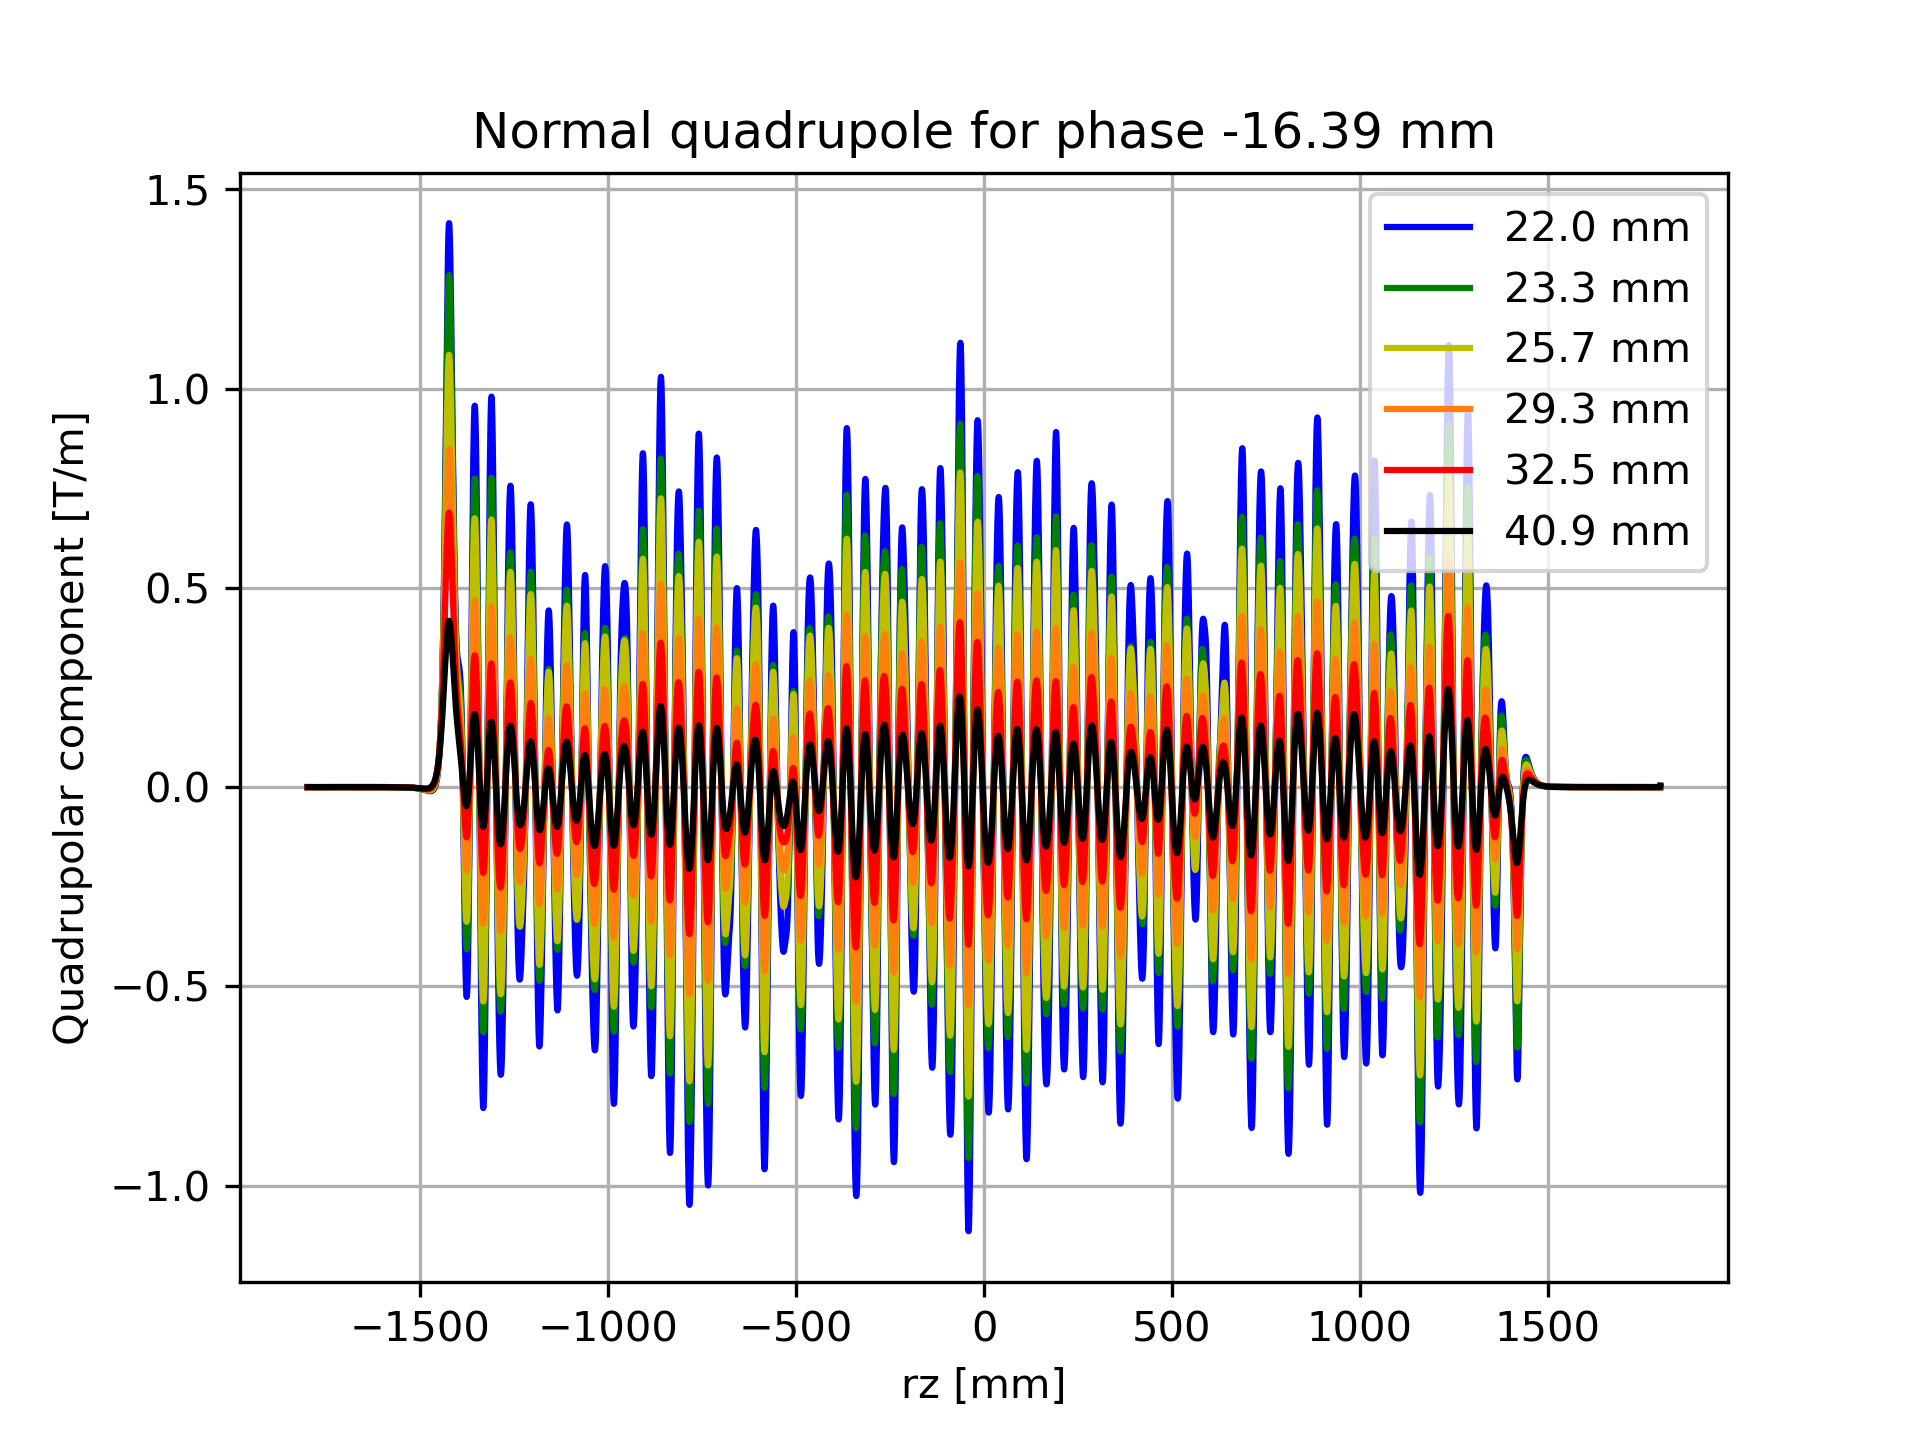
\includegraphics[width=0.9\linewidth, height=7cm]{figs/phase-16 Normal quadrupole.png} 
\label{fig:subim1-16q}
\end{subfigure}
\begin{subfigure}{0.5\textwidth}
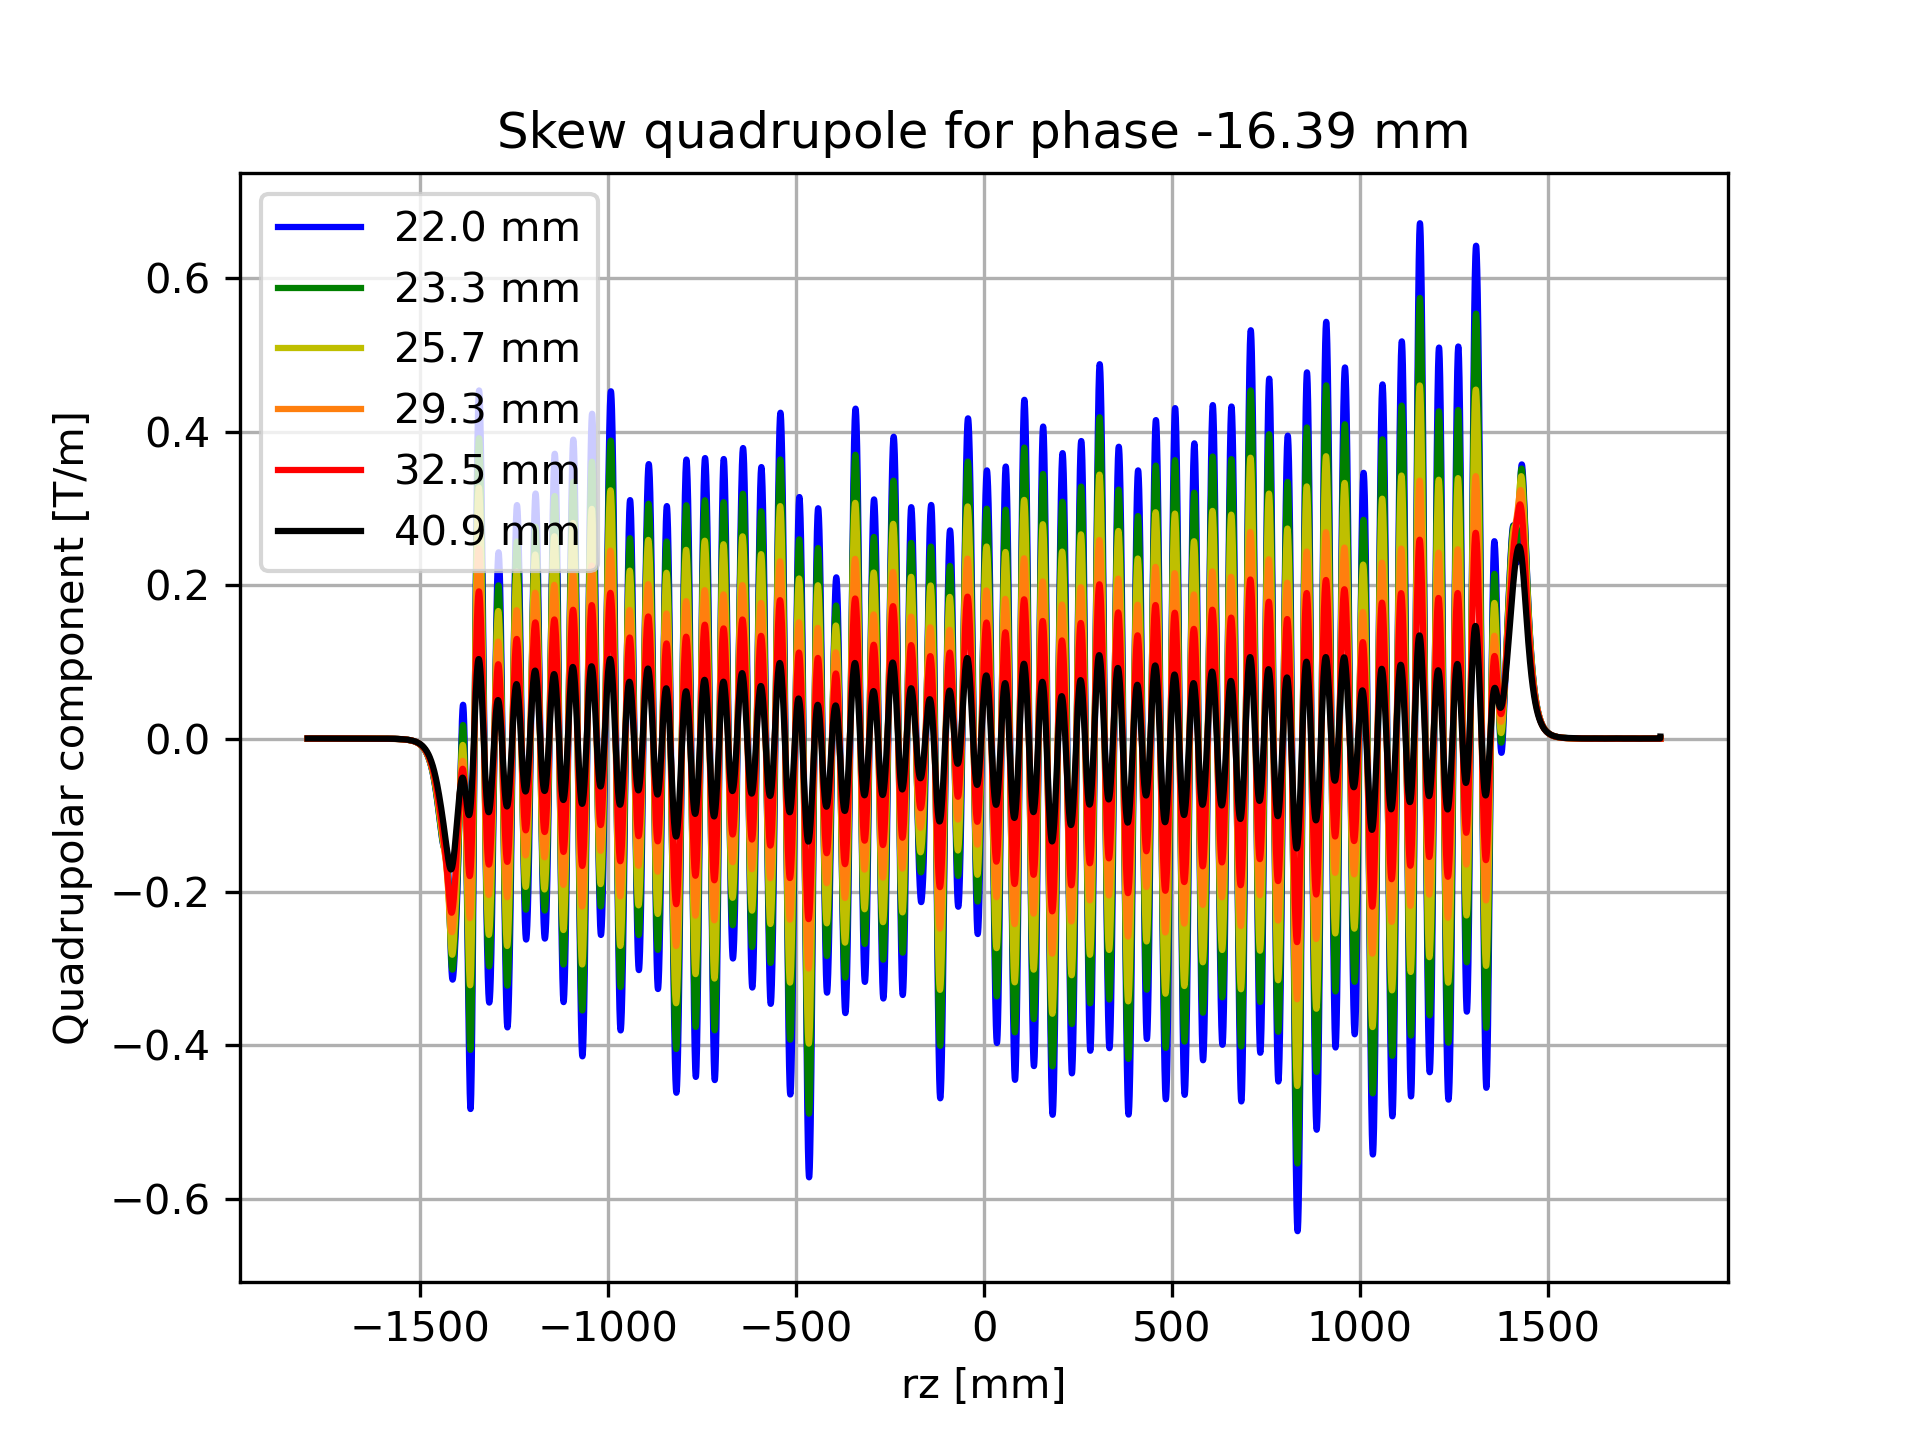
\includegraphics[width=0.9\linewidth, height=7cm]{figs/phase-16 Skew quadrupole.png}
\label{fig:subim2-16q}
\end{subfigure}
\caption{Componentes quadrupolares de campo}
\label{fig:quad-16}
\end{figure}

\begin{figure}[H]
\begin{subfigure}{0.5\textwidth}
\includegraphics[width=0.9\linewidth, height=7cm]{figs/phase-16 Normal sextupole.png} 
\label{fig:subim1-16s}
\end{subfigure}
\begin{subfigure}{0.5\textwidth}
\includegraphics[width=0.9\linewidth, height=7cm]{figs/phase-16 Skew sextupole.png}
\label{fig:subim2-16s}
\end{subfigure}
\caption{Componentes sextupolares de campo}
\label{fig:sext-16}
\end{figure}

Os valores dos multipolos integrados para esta fase encontram-se detalhados na tabela abaixo.

\begin{table}[H]\footnotesize
\caption{Integrais das componentes multipolares}
\centering
\begin{tabular}{|c|c|c|c|c|}
\hline
   Gap [mm] &   Normal quadrupole [T] &   Skew quadrupole [T] &   Normal sextupole [T/m] &   Skew sextupole [T/m] \\
\hline
22.0 & +0.0175 & +0.0024 & +0.6014 & -0.8092 \\
23.3 & +0.0148 & +0.0019 & +0.3391 & -0.6958 \\
25.7 & +0.0116 & +0.0013 & +0.5316 & -0.5389 \\
29.3 & +0.0082 & +0.0003 & +0.2060 & -0.4226 \\
32.5 & +0.0064 & -0.0000 & +0.1783 & -0.2095 \\
40.9 & +0.0022 & -0.0005 & +0.2274 & +0.0801 \\
\hline
\end{tabular}
\end{table}





\subsection{Fase 16.39 mm}

\subsubsection{Campo vs gap}
\begin{figure}[H]
\hspace{4cm}
\includegraphics[width=0.5\textwidth]{figs/phase16 B vs gap.png}
\caption{Beff vs gap fase = 16.39 mm}
\label{fig:fieldgap16}
\end{figure}

\begin{table}[H]
\caption{Beff vs gap fase = 16.39 mm}
\centering
\begin{tabular}{|c|c|c|}
\hline
   Gap [mm] &   Bx [T] &   By [T] \\
\hline
       22.0 &     0.23 &     0.24 \\
       23.3 &     0.21 &     0.22 \\
       25.7 &     0.17 &     0.19 \\
       29.3 &     0.13 &     0.15 \\
       32.5 &    0.10 &    0.13 \\
       40.9 &     0.05 &     0.07 \\
\hline
\end{tabular}
\end{table}

\paragraph{} As figuras abaixo exibem os campos normalizados do ID na configuração em questão.

\begin{figure}[H]
\begin{subfigure}{0.5\textwidth}
\includegraphics[width=0.9\linewidth, height=7cm]{figs/phase16 Bx.png} 
\label{fig:subim116}
\end{subfigure}
\begin{subfigure}{0.5\textwidth}
\includegraphics[width=0.9\linewidth, height=7cm]{figs/phase16 By.png}
\label{fig:subim216}
\end{subfigure}
\caption{Componentes de campo horizontais (esquerda) e verticais (direita)}
\label{fig:bx_by_16}
\end{figure}


\begin{figure}[H]
\begin{center}
\includegraphics[width=0.5\textwidth]{figs/phase16 Bz.png}
\caption{Componente longitudinal de campo normalizada}
\label{fig:bz_16}
\end{center}
\end{figure}

\subsubsection{Correções de órbita}



\begin{table}[H]
\centering
\caption{Tabela de correção local}
\begin{tabular}{|c|c|c|c|c|}
\hline
Gap {[}mm{]} & $\Delta$px up {[}$\mu$rad{]} & $\Delta$px down {[}$\mu$rad{]} & $\Delta$py up {[}$\mu$rad{]} & $\Delta$py down {[}$\mu$rad{]} \\ \hline
22.0 & 6.41 & -2.24 & -12.81 & -10.16 \\ \hline
23.3 & 5.69  & -2.52 & -10.36 & -9.21 \\ \hline
25.7 & 5.07 & -2.50 & -8.46 & -9.62 \\ \hline
29.3 & 3.74  & -2.80 & -5.22 & -9.36 \\ \hline
32.5 &  3.08 & -2.53  & -3.03  & -9.21 \\ \hline
40.9 & 1.14  & -2.41 & 0.42 & -9.04 \\ \hline
\end{tabular}
\label{tab:corff16}
\end{table}


Os gráficos das figuras \ref{fig:-16corrx} e \ref{fig:-16corry} exibem a trajetória média após a correção com FOFB (gráficos da esquerda) e correções locais (gráficos da direita).

\begin{figure}[H]
\begin{subfigure}{0.5\textwidth}
\includegraphics[width=0.9\linewidth, height=7cm]{figs/phase16 horizontal-avg-traj-FOFB.png} 
\label{fig:subim10xc16}
\end{subfigure}
\begin{subfigure}{0.5\textwidth}
\includegraphics[width=0.9\linewidth, height=7cm]{figs/phase16 horizontal-avg-traj-LOCAL.png}
\label{fig:subim20xc16}
\end{subfigure}
\caption{Trajetória média horizontal após correções de órbita utilizando FOFB (esquerda) e feedforward (direita)}
\label{fig:16corrx}
\end{figure}

\begin{figure}[H]
\begin{subfigure}{0.5\textwidth}
\includegraphics[width=0.9\linewidth, height=7cm]{figs/phase16 vertical-avg-traj-FOFB.png} 
\label{fig:subim10yc16}
\end{subfigure}
\begin{subfigure}{0.5\textwidth}
\includegraphics[width=0.9\linewidth, height=7cm]{figs/phase16 vertical-avg-traj-LOCAL.png}
\label{fig:subim20yc16}
\end{subfigure}
\caption{Trajetória média vertical após correções de órbita utilizando FOFB (esquerda) e feedforward (direita)}
\label{fig:16corry}
\end{figure}



\subsubsection{Trajetória}

\begin{figure}[H]
\begin{subfigure}{0.5\textwidth}
\includegraphics[width=0.9\linewidth, height=7cm]{figs/phase16 RK Posx.png} 
\label{fig:subim116tx}
\end{subfigure}
\begin{subfigure}{0.5\textwidth}
\includegraphics[width=0.9\linewidth, height=7cm]{figs/phase16 RK Angx.png}
\label{fig:subim216tx}
\end{subfigure}
\caption{Trajetória X para fase 16.39 mm}
\label{fig:trajx_16}
\end{figure}

\begin{figure}[H]
\begin{subfigure}{0.5\textwidth}
\includegraphics[width=0.9\linewidth, height=7cm]{figs/phase16 RK Posy.png} 
\label{fig:subim116ty}
\end{subfigure}
\begin{subfigure}{0.5\textwidth}
\includegraphics[width=0.9\linewidth, height=7cm]{figs/phase16 RK Angy.png}
\label{fig:subim216ty}
\end{subfigure}
\caption{Trajetória Y para fase 16.39 mm}
\label{fig:trajy_16}
\end{figure}

Os valores finais de ângulo e trajetória mostrados nas figuras acima estão resumidos nas tabelas abaixo, em conjunto com as integrais de campo.


\begin{table}[H]
\centering
\caption{Primeiras integrais de campo}
\begin{tabular}{|c|c|c|}
\hline
   Gap [mm] & Bx 1st integral [G cm] / $\Delta$ py [$\mu$rad] & By 1st integral [G cm] / $\Delta$ px [$\mu$rad] \\
\hline
    22.0 & -227.5 / +22.63 & -33.8 / -3.16 \\
    23.3 & -190.7 / +18.95 & -22.4 / -2.06 \\
    25.7 & -176.8 / +17.61 & -15.9 / -1.47 \\
    29.3 & -140.6 / +14.02 &  +2.0 / +0.27 \\
    32.5 & -116.7 / +11.64 &  +5.8 / +0.62 \\
    40.9 & -80.5 / +8.04 & +24.6 / +2.47 \\
\hline
\end{tabular}
\end{table}

\begin{table}[H]
\centering
\caption{Segundas integrais de campo}
\begin{tabular}{|c|c|c|}
\hline
   Gap [mm] & Bx 2nd integral [G cm²] / $\Delta$ y [$\mu$m] & By 2nd integral [G cm²] / $\Delta$ x [$\mu$m]   \\
\hline
    22.0 & -4.64e+04 / +46.20 & -2.14e+04 / -20.96 \\
    23.3 & -3.74e+04 / +37.20 & -1.86e+04 / -18.26 \\
    25.7 & -3.11e+04 / +31.00 & -1.64e+04 / -16.16 \\
    29.3 & -1.98e+04 / +19.71 & -1.15e+04 / -11.41 \\
    32.5 & -1.22e+04 / +12.15 & -9.37e+03 / -9.30 \\
    40.9 & -3.05e+02 / +0.29 & -2.74e+03 / -2.72 \\
\hline
\end{tabular}
\end{table}


\subsubsection{Multipolos}
As figuras abaixo exibem os multipolos ao longo da trajetória do elétron no ID para diversos gaps.

\begin{figure}[H]
\begin{subfigure}{0.5\textwidth}
\includegraphics[width=0.9\linewidth, height=7cm]{figs/phase16 Normal quadrupole.png} 
\label{fig:subim116q}
\end{subfigure}
\begin{subfigure}{0.5\textwidth}
\includegraphics[width=0.9\linewidth, height=7cm]{figs/phase16 Skew quadrupole.png}
\label{fig:subim216q}
\end{subfigure}
\caption{Componentes quadrupolares de campo}
\label{fig:quad16}
\end{figure}

\begin{figure}[H]
\begin{subfigure}{0.5\textwidth}
\includegraphics[width=0.9\linewidth, height=7cm]{figs/phase16 Normal sextupole.png} 
\label{fig:subim116s}
\end{subfigure}
\begin{subfigure}{0.5\textwidth}
\includegraphics[width=0.9\linewidth, height=7cm]{figs/phase16 Skew sextupole.png}
\label{fig:subim216s}
\end{subfigure}
\caption{Componentes sextupolares de campo}
\label{fig:sext16}
\end{figure}

Os valores dos multipolos integrados para esta fase encontram-se detalhados na tabela abaixo.

\begin{table}[H]\footnotesize
\caption{Integrais das componentes multipolares}
\centering
\begin{tabular}{|c|c|c|c|c|}
\hline
   Gap [mm] &   Normal quadrupole [T] &   Skew quadrupole [T] &   Normal sextupole [T/m] &   Skew sextupole [T/m] \\
\hline
22.0 & +0.0159 & -0.0027 & +0.6605 & +1.8722 \\
23.3 & +0.0142 & -0.0024 & +0.5638 & +1.6695 \\
25.7 & +0.0106 & -0.0025 & +0.4100 & +1.3513 \\
29.3 & +0.0077 & -0.0024 & +0.3266 & +0.7606 \\
32.5 & +0.0051 & -0.0023 & +0.3596 & +0.5711 \\
40.9 & +0.0020 & -0.0020 & +0.0582 & +0.2692 \\
\hline
\end{tabular}
\end{table}





\subsection{Fase -25.00 mm}

\subsubsection{Campo vs gap}

\begin{figure}[H]
\hspace{4cm}
\includegraphics[width=0.5\textwidth]{figs/phase-25 B vs gap.png}
\caption{Beff vs gap fase = -25 mm}
\label{fig:fieldgap-25}
\end{figure}

\begin{table}[H]
\caption{Beff vs gap fase = -25 mm}
\centering
\begin{tabular}{|c|c|}
\hline
   Gap [mm] &   Bx [T] \\
\hline
       22.0   &     0.27      \\
       23.3 &     0.25      \\
       25.7 &     0.20       \\
       29.3 &     0.15      \\
       32.5 &     0.12          \\
       40.9 &     0.06          \\
\hline
\end{tabular}
\end{table}

\paragraph{} As figuras abaixo exibem os campos normalizados do ID na configuração em questão.

\begin{figure}[H]
\begin{center}
\includegraphics[width=0.5\textwidth]{figs/phase-25 Bx.png}
\caption{Componente horizontal de campo normalizada}
\label{fig:bx-25}
\end{center}
\end{figure}


\begin{figure}[H]
\begin{subfigure}{0.5\textwidth}
\includegraphics[width=0.9\linewidth, height=7cm]{figs/phase-25 By.png} 
\label{fig:subim1-25}
\end{subfigure}
\begin{subfigure}{0.5\textwidth}
\includegraphics[width=0.9\linewidth, height=7cm]{figs/phase-25 Bz.png}
\label{fig:subim2-25}
\end{subfigure}
\caption{Componentes de campo verticais (esquerda) e longitudinais (direita)}
\label{fig:by_bz-25}
\end{figure}

\subsubsection{Correções de órbita}

\begin{table}[H]
\centering
\caption{Tabela de correção local}
\begin{tabular}{|c|c|c|c|c|}
\hline
Gap {[}mm{]} & $\Delta$px up {[}$\mu$rad{]} & $\Delta$px down {[}$\mu$rad{]} & $\Delta$py up {[}$\mu$rad{]} & $\Delta$py down {[}$\mu$rad{]} \\ \hline
22.0 & 4.45  & -2.75 & 0.23 & 2.87 \\ \hline
23.3 & 3.93 & -3.05 & 1.65 & 2.66 \\ \hline
25.7 & 3.50  & -3.07 & 2.24 & 0.75 \\ \hline
29.3 & 2.57  & -3.24 & 3.73 & -0.89 \\ \hline
32.5 & 2.03  & -3.05 & 4.76 & -1.95 \\ \hline
40.9 & 0.29  & -2.99 & 6.35 & -3.63 \\ \hline
\end{tabular}
\label{tab:corff-25}
\end{table}

Os gráficos das figuras \ref{fig:-25corrx} e \ref{fig:-25corry} exibem a trajetória média após a correção com FOFB (gráficos da esquerda) e correções locais (gráficos da direita).

\begin{figure}[H]
\begin{subfigure}{0.5\textwidth}
\includegraphics[width=0.9\linewidth, height=7cm]{figs/phase-25 horizontal-avg-traj-FOFB.png} 
\label{fig:subim10xc-25}
\end{subfigure}
\begin{subfigure}{0.5\textwidth}
\includegraphics[width=0.9\linewidth, height=7cm]{figs/phase-25 horizontal-avg-traj-LOCAL.png}
\label{fig:subim20xc-25}
\end{subfigure}
\caption{Trajetória média horizontal após correções de órbita utilizando FOFB (esquerda) e feedforward (direita)}
\label{fig:-25corrx}
\end{figure}

\begin{figure}[H]
\begin{subfigure}{0.5\textwidth}
\includegraphics[width=0.9\linewidth, height=7cm]{figs/phase-25 vertical-avg-traj-FOFB.png} 
\label{fig:subim10yc25}
\end{subfigure}
\begin{subfigure}{0.5\textwidth}
\includegraphics[width=0.9\linewidth, height=7cm]{figs/phase-25 vertical-avg-traj-LOCAL.png}
\label{fig:subim20yc25}
\end{subfigure}
\caption{Trajetória média vertical após correções de órbita utilizando FOFB (esquerda) e feedforward (direita)}
\label{fig:-25corry}
\end{figure}


\subsubsection{Trajetória}


\begin{figure}[H]
\begin{subfigure}{0.5\textwidth}
\includegraphics[width=0.9\linewidth, height=7cm]{figs/phase-25 RK Posx.png} 
\label{fig:subim1-25tx}
\end{subfigure}
\begin{subfigure}{0.5\textwidth}
\includegraphics[width=0.9\linewidth, height=7cm]{figs/phase-25 RK Angx.png}
\label{fig:subim2-25tx}
\end{subfigure}
\caption{Trajetória X para fase -25 mm}
\label{fig:trajx-25}
\end{figure}

\begin{figure}[H]
\begin{subfigure}{0.5\textwidth}
\includegraphics[width=0.9\linewidth, height=7cm]{figs/phase-25 RK Posy.png} 
\label{fig:subim1-25ty}
\end{subfigure}
\begin{subfigure}{0.5\textwidth}
\includegraphics[width=0.9\linewidth, height=7cm]{figs/phase-25 RK Angy.png}
\label{fig:subim2-25ty}
\end{subfigure}
\caption{Trajetória Y para fase -25 mm}
\label{fig:trajy-25}
\end{figure}

Os valores finais de ângulo e trajetória mostrados nas figuras acima estão resumidos nas tabelas abaixo, em conjunto com as integrais de campo.


\begin{table}[H]
\centering
\caption{Primeiras integrais de campo}
\begin{tabular}{|c|c|c|}
\hline
   Gap [mm] & Bx 1st integral [G cm] / $\Delta$ py [$\mu$rad] & By 1st integral [G cm] / $\Delta$ px [$\mu$rad] \\
\hline
        22.0 & +33.6 / -3.37 & -11.3 / -0.76 \\
        23.3 & +48.2 / -4.83 &  -1.7 / +0.12 \\
        25.7 & +33.8 / -3.39 &  +3.0 / +0.50 \\
        29.3 & +32.7 / -3.27 & +15.0 / +1.61 \\
        32.5 & +32.5 / -3.25 & +18.4 / +1.90 \\
        40.9 & +31.9 / -3.19 & +36.0 / +3.62 \\
\hline
\end{tabular}
\end{table}

\begin{table}[H]
\centering
\caption{Segundas integrais de campo}
\begin{tabular}{|c|c|c|}
\hline
   Gap [mm] & Bx 2nd integral [G cm²] / $\Delta$ y [$\mu$m] & By 2nd integral [G cm²] / $\Delta$ x [$\mu$m]   \\
\hline
        22.0 & +2.11e+03 / -2.12 & -1.46e+04 / -13.94 \\
        23.3 & +7.23e+03 / -7.25 & -1.26e+04 / -12.04 \\
        25.7 & +8.54e+03 / -8.55 & -1.10e+04 / -10.67 \\
        29.3 & +1.32e+04 / -13.25 & -7.64e+03 / -7.44 \\
        32.5 & +1.65e+04 / -16.49 & -5.87e+03 / -5.75 \\
        40.9 & +2.15e+04 / -21.54 & +2.04e+02 / +0.24 \\
\hline
\end{tabular}
\end{table}

\subsubsection{Multipolos}
As figuras abaixo exibem os multipolos ao longo da trajetória do elétron no ID para diversos gaps.

\begin{figure}[H]
\begin{subfigure}{0.5\textwidth}
\includegraphics[width=0.9\linewidth, height=7cm]{figs/phase-25 Normal quadrupole.png} 
\label{fig:subim1-25q}
\end{subfigure}
\begin{subfigure}{0.5\textwidth}
\includegraphics[width=0.9\linewidth, height=7cm]{figs/phase-25 Skew quadrupole.png}
\label{fig:subim2-25q}
\end{subfigure}
\caption{Componentes quadrupolares de campo}
\label{fig:quad-25}
\end{figure}

\begin{figure}[H]
\begin{subfigure}{0.5\textwidth}
\includegraphics[width=0.9\linewidth, height=7cm]{figs/phase-25 Normal sextupole.png} 
\label{fig:subim1-25s}
\end{subfigure}
\begin{subfigure}{0.5\textwidth}
\includegraphics[width=0.9\linewidth, height=7cm]{figs/phase-25 Skew sextupole.png}
\label{fig:subim2-25s}
\end{subfigure}
\caption{Componentes sextupolares de campo}
\label{fig:sext-25}
\end{figure}

Os valores dos multipolos integrados para esta fase encontram-se detalhados na tabela abaixo.

\begin{table}[H]\footnotesize
\caption{Integrais das componentes multipolares}
\centering
\begin{tabular}{|c|c|c|c|c|}
\hline
   Gap [mm] &   Normal quadrupole [T] &   Skew quadrupole [T] &   Normal sextupole [T/m] &   Skew sextupole [T/m] \\
\hline
        22.0 & +0.0164 & -0.0020 & +0.1887 & +0.4409 \\
        23.3 & +0.0145 & -0.0015 & +0.6119 & +0.4303 \\
        25.7 & +0.0113 & -0.0017 & +0.3960 & +0.4033 \\
        29.3 & +0.0079 & -0.0014 & +0.4576 & +0.2011 \\
        32.5 & +0.0062 & -0.0013 & +0.3254 & +0.1177 \\
        40.9 & +0.0027 & -0.0015 & +0.1970 & -0.0181 \\
\hline
\end{tabular}
\end{table}




\subsection{Fase 25.00 mm}

\subsubsection{Campo vs gap}
\begin{figure}[H]
\hspace{4cm}
\includegraphics[width=0.5\textwidth]{figs/phase25 B vs gap.png}
\caption{Beff vs gap fase = 25.00 mm}
\label{fig:fiedlgap25}
\end{figure}

\begin{table}[H]
\caption{Beff vs gap fase = 25.00 mm}
\centering
\begin{tabular}{|c|c|c|}
\hline
   Gap [mm] &   Bx [T]  \\
\hline
       22.0   &     0.27       \\
       23.3 &     0.25       \\
       25.7 &     0.20       \\
       29.3 &     0.15       \\
       32.5 &     0.12         \\
       40.9 &     0.06          \\
\hline
\end{tabular}
\end{table}

\paragraph{} As figuras abaixo exibem os campos normalizados do ID na configuração em questão.


\begin{figure}[H]
\begin{center}
\includegraphics[width=0.5\textwidth]{figs/phase25 Bx.png}
\caption{Componente horizontal de campo normalizada}
\label{fig:bx_25}
\end{center}
\end{figure}

\begin{figure}[H]
\begin{subfigure}{0.5\textwidth}
\includegraphics[width=0.9\linewidth, height=7cm]{figs/phase25 By.png} 
\label{fig:subim125}
\end{subfigure}
\begin{subfigure}{0.5\textwidth}
\includegraphics[width=0.9\linewidth, height=7cm]{figs/phase25 Bz.png}
\label{fig:subim225}
\end{subfigure}
\caption{Componentes de campo verticais (esquerda) e longitudinais (direita)}
\label{fig:by_bz_25}
\end{figure}

\subsubsection{Correções de órbita}

\begin{table}[H]
\centering
\caption{Tabela de correção local}
\begin{tabular}{|c|c|c|c|c|}
\hline
Gap {[}mm{]} & $\Delta$px up {[}$\mu$rad{]} & $\Delta$px down {[}$\mu$rad{]} & $\Delta$py up {[}$\mu$rad{]} & $\Delta$py down {[}$\mu$rad{]} \\ \hline
22.0 & 4.90 & -1.17 & -7.26 & -6.79 \\ \hline
23.3 & 4.29  & -1.51 & -5.33 & -6.42 \\ \hline
25.7 & 4.00  & -1.43 & -3.99 & -7.44 \\ \hline
29.3 & 2.77  & -1.91 & -1.46 & -7.82 \\ \hline
32.5 &  2.07 & -1.83 & 0.24 & -8.09  \\ \hline
40.9 & 0.49  & -1.74 & 2.94 & -8.35 \\ \hline
\end{tabular}
\label{tab:corff25}
\end{table}

Os gráficos das figuras \ref{fig:25corrx} e \ref{fig:25corry} exibem a trajetória média após a correção com FOFB (gráficos da esquerda) e correções locais (gráficos da direita).

\begin{figure}[H]
\begin{subfigure}{0.5\textwidth}
\includegraphics[width=0.9\linewidth, height=7cm]{figs/phase25 horizontal-avg-traj-FOFB.png} 
\label{fig:subim10xc25}
\end{subfigure}
\begin{subfigure}{0.5\textwidth}
\includegraphics[width=0.9\linewidth, height=7cm]{figs/phase25 horizontal-avg-traj-LOCAL.png}
\label{fig:subim20xc25}
\end{subfigure}
\caption{Trajetória média horizontal após correções de órbita utilizando FOFB (esquerda) e feedforward (direita)}
\label{fig:25corrx}
\end{figure}

\begin{figure}[H]
\begin{subfigure}{0.5\textwidth}
\includegraphics[width=0.9\linewidth, height=7cm]{figs/phase25 vertical-avg-traj-FOFB.png} 
\label{fig:subim10yc25}
\end{subfigure}
\begin{subfigure}{0.5\textwidth}
\includegraphics[width=0.9\linewidth, height=7cm]{figs/phase25 vertical-avg-traj-LOCAL.png}
\label{fig:subim20yc25}
\end{subfigure}
\caption{Trajetória média vertical após correções de órbita utilizando FOFB (esquerda) e feedforward (direita)}
\label{fig:25corry}
\end{figure}



\subsubsection{Trajetória}


\begin{figure}[H]
\begin{subfigure}{0.5\textwidth}
\includegraphics[width=0.9\linewidth, height=7cm]{figs/phase25 RK Posx.png} 
\label{fig:subim125tx}
\end{subfigure}
\begin{subfigure}{0.5\textwidth}
\includegraphics[width=0.9\linewidth, height=7cm]{figs/phase25 RK Angx.png}
\label{fig:subim225tx}
\end{subfigure}
\caption{Trajetória X para fase 25.00 mm}
\label{fig:trajx_25}
\end{figure}

\begin{figure}[H]
\begin{subfigure}{0.5\textwidth}
\includegraphics[width=0.9\linewidth, height=7cm]{figs/phase25 RK Posy.png} 
\label{fig:subim125ty}
\end{subfigure}
\begin{subfigure}{0.5\textwidth}
\includegraphics[width=0.9\linewidth, height=7cm]{figs/phase25 RK Angy.png}
\label{fig:subim225ty}
\end{subfigure}
\caption{Trajetória Y para fase 25.00 mm}
\label{fig:trajy_25}
\end{figure}

Os valores finais de ângulo e trajetória mostrados nas figuras acima estão resumidos nas tabelas abaixo, em conjunto com as integrais de campo.


\begin{table}[H]
\centering
\caption{Primeiras integrais de campo}
\begin{tabular}{|c|c|c|}
\hline
   Gap [mm] & Bx 1st integral [G cm] / $\Delta$ py [$\mu$rad] & By 1st integral [G cm] / $\Delta$ px [$\mu$rad] \\
\hline
    22.0 & -135.2 / +13.51 & -28.7 / -2.50 \\
    23.3 & -110.1 / +11.00 & -18.0 / -1.50 \\
    25.7 & -108.4 / +10.83 & -15.6 / -1.37 \\
    29.3 & -86.1 / +8.61 &  +3.3 / +0.44 \\
    32.5 & -71.7 / +7.16 &  +9.7 / +1.04 \\
    40.9 & -47.2 / +4.72 & +25.2 / +2.54 \\
\hline
\end{tabular}
\end{table}

\begin{table}[H]
\centering
\caption{Segundas integrais de campo}
\begin{tabular}{|c|c|c|}
\hline
   Gap [mm] & Bx 2nd integral [G cm²] / $\Delta$ y [$\mu$m] & By 2nd integral [G cm²] / $\Delta$ x [$\mu$m]   \\
\hline
    22.0 & -2.61e+04 / +26.12 & -1.65e+04 / -15.83 \\
    23.3 & -1.91e+04 / +19.10 & -1.41e+04 / -13.58 \\
    25.7 & -1.50e+04 / +15.02 & -1.31e+04 / -12.74 \\
    29.3 & -6.38e+03 / +6.37 & -8.52e+03 / -8.32 \\
    32.5 & -6.20e+02 / +0.62 & -6.10e+03 / -5.98 \\
    40.9 & +8.59e+03 / -8.59 & -7.19e+02 / -0.69 \\
\hline
\end{tabular}
\end{table}

\subsubsection{Multipolos}
As figuras abaixo exibem os multipolos ao longo da trajetória do elétron no ID para diversos gaps.

\begin{figure}[H]
\begin{subfigure}{0.5\textwidth}
\includegraphics[width=0.9\linewidth, height=7cm]{figs/phase25 Normal quadrupole.png} 
\label{fig:subim125q}
\end{subfigure}
\begin{subfigure}{0.5\textwidth}
\includegraphics[width=0.9\linewidth, height=7cm]{figs/phase25 Skew quadrupole.png}
\label{fig:sub1quad_25}
\end{subfigure}
\caption{Componentes quadrupolares de campo}
\label{fig:quad_25}
\end{figure}

\begin{figure}[H]
\begin{subfigure}{0.5\textwidth}
\includegraphics[width=0.9\linewidth, height=7cm]{figs/phase25 Normal sextupole.png} 
\label{fig:subim125s}
\end{subfigure}
\begin{subfigure}{0.5\textwidth}
\includegraphics[width=0.9\linewidth, height=7cm]{figs/phase25 Skew sextupole.png}
\label{fig:subim225s}
\end{subfigure}
\caption{Componentes sextupolares de campo}
\label{fig:sext25}
\end{figure}

Os valores dos multipolos integrados para esta fase encontram-se detalhados na tabela abaixo.

\begin{table}[H]\footnotesize
\caption{Integrais das componentes multipolares}
\centering
\begin{tabular}{|c|c|c|c|c|}
\hline
   Gap [mm] &   Normal quadrupole [T] &   Skew quadrupole [T] &   Normal sextupole [T/m] &   Skew sextupole [T/m] \\
\hline
22.0 & +0.0169 & -0.0019 & +0.2860 & +0.9940 \\
23.3 & +0.0151 & -0.0024 & +0.6635 & +0.7948 \\
25.7 & +0.0121 & -0.0023 & +0.7180 & +0.5893 \\
29.3 & +0.0085 & -0.0021 & +0.2052 & +0.4706 \\
32.5 & +0.0067 & -0.0024 & +0.1528 & +0.4185 \\
40.9 & +0.0027 & -0.0021 & +0.1737 & +0.2311 \\
\hline
\end{tabular}
\end{table}

\section{Análise de óptica}
\subsection{Correções}
\subsubsection{Fase 00.00 mm}

Além da análise de campos, também foi verificado o efeito do EPU na óptica do SIRIUS, para isso foram realizadas simulações utilizando o modelo computacional do anél de armazenamento. Os desvios de sintonia para cada gap da fase em questão estão detalhados na tabela \ref{tab:coropt0}.

\begin{table}[H]
\centering
\caption{Desvio de sintonia}
\begin{tabular}{|c|c|c|c|c|}
\hline
Gap {[}mm{]} & $\Delta \nu$x & $\Delta \nu$y\\ \hline
22.0 & +6e-05 & 0\\ \hline
23.3 & +7e-05 & 0\\ \hline
25.7 & +2e-05 & 0\\ \hline
29.3 & +8e-06 & 0\\ \hline
32.5 & -2e-05 & 0\\ \hline
40.9 & +6e-06 & 0\\ \hline
\end{tabular}
\label{tab:coropt0}
\end{table}

\paragraph{} O gap nominal de operação do ID foi configurado para 36mm, o que garante uma amplitude de campo de 2T, nesse configuração não foi observado desvio de sintonia durante o comissionamento, o que está de acordo com os resultados da tabela \ref{tab:coropt0}.

As figuras abaixo exibem o beta beating antes e após a simetrização da óptica e correção de sintonias para cada gap.

\textbf{Gap 22.0 mm} \\

\begin{figure}[H]
\begin{subfigure}{0.5\textwidth}
\includegraphics[width=0.9\linewidth, height=7cm]{figs/phase0 gap22 uncorrected-optics.png} 
\label{fig:subim1022}
\end{subfigure}
\begin{subfigure}{0.5\textwidth}
\includegraphics[width=0.9\linewidth, height=7cm]{figs/phase0 gap22 corrected-optics-tunes.png}
\label{fig:subim2022}
\end{subfigure}
\caption{Beta beating antes da correção (esquerda) e após correção (direita) - gap 22.0 mm}
\label{fig:bb0_22}
\end{figure}

\textbf{Gap 23.3 mm} \\

\begin{figure}[H]
\begin{subfigure}{0.5\textwidth}
\includegraphics[width=0.9\linewidth, height=7cm]{figs/phase0 gap23 uncorrected-optics.png} 
\label{fig:subim1023}
\end{subfigure}
\begin{subfigure}{0.5\textwidth}
\includegraphics[width=0.9\linewidth, height=7cm]{figs/phase0 gap23 corrected-optics-tunes.png}
\label{fig:subim2023}
\end{subfigure}
\caption{Beta beating antes da correção (esquerda) e após correção (direita) - gap 23.3 mm}
\label{fig:bb0_23}
\end{figure}

\textbf{Gap 25.7 mm} \\

\begin{figure}[H]
\begin{subfigure}{0.5\textwidth}
\includegraphics[width=0.9\linewidth, height=7cm]{figs/phase0 gap25 uncorrected-optics.png} 
\label{fig:subim1025}
\end{subfigure}
\begin{subfigure}{0.5\textwidth}
\includegraphics[width=0.9\linewidth, height=7cm]{figs/phase0 gap25 corrected-optics-tunes.png}
\label{fig:subim2025}
\end{subfigure}
\caption{Beta beating antes da correção (esquerda) e após correção (direita) - gap 25.7 mm}
\label{fig:bb0_25}
\end{figure}

\textbf{Gap 29.3 mm} \\

\begin{figure}[H]
\begin{subfigure}{0.5\textwidth}
\includegraphics[width=0.9\linewidth, height=7cm]{figs/phase0 gap29 uncorrected-optics.png} 
\label{fig:subim1029}
\end{subfigure}
\begin{subfigure}{0.5\textwidth}
\includegraphics[width=0.9\linewidth, height=7cm]{figs/phase0 gap29 corrected-optics-tunes.png}
\label{fig:subim2029}
\end{subfigure}
\caption{Beta beating antes da correção (esquerda) e após correção (direita) - gap 29.3 mm}
\label{fig:bb0_29}
\end{figure}

\textbf{Gap 32.5 mm} \\

\begin{figure}[H]
\begin{subfigure}{0.5\textwidth}
\includegraphics[width=0.9\linewidth, height=7cm]{figs/phase0 gap32 uncorrected-optics.png} 
\label{fig:subim1032}
\end{subfigure}
\begin{subfigure}{0.5\textwidth}
\includegraphics[width=0.9\linewidth, height=7cm]{figs/phase0 gap32 corrected-optics-tunes.png}
\label{fig:subim2032}
\end{subfigure}
\caption{Beta beating antes da correção (esquerda) e após correção (direita) - gap 32.5 mm}
\label{fig:bb0_32}
\end{figure}

\textbf{Gap 40.9 mm} \\

\begin{figure}[H]
\begin{subfigure}{0.5\textwidth}
\includegraphics[width=0.9\linewidth, height=7cm]{figs/phase0 gap40 uncorrected-optics.png} 
\label{fig:subim1040}
\end{subfigure}
\begin{subfigure}{0.5\textwidth}
\includegraphics[width=0.9\linewidth, height=7cm]{figs/phase0 gap40 corrected-optics-tunes.png}
\label{fig:subim2040}
\end{subfigure}
\caption{Beta beating antes da correção (esquerda) e após correção (direita) - gap 40.9 mm}
\label{fig:bb0_40}
\end{figure}

\subsubsection{Fase -16.39 mm}

\begin{table}[H]
\centering
\caption{Desvio de sintonia}
\begin{tabular}{|c|c|c|c|c|}
\hline
Gap {[}mm{]} & $\Delta \nu$x & $\Delta \nu$y\\ \hline
22.0 & -5e-05 & 0\\ \hline
23.3 & -4e-05 & 0\\ \hline
25.7 & -4e-05 & 0\\ \hline
29.3 & -6e-05 & 0\\ \hline
32.5 & -6e-05 & 0 \\ \hline
40.9 & -8e-06 & 0\\ \hline
\end{tabular}
\label{tab:coropt-16}
\end{table}

\textbf{Gap 22.0 mm} \\

\begin{figure}[H]
\begin{subfigure}{0.5\textwidth}
\includegraphics[width=0.9\linewidth, height=7cm]{figs/phase-16 gap22 uncorrected-optics.png} 
\label{fig:subim1-1622}
\end{subfigure}
\begin{subfigure}{0.5\textwidth}
\includegraphics[width=0.9\linewidth, height=7cm]{figs/phase-16 gap22 corrected-optics-tunes.png}
\label{fig:subim2-1622}
\end{subfigure}
\caption{Beta beating antes da correção (esquerda) e após correção (direita) - gap 22.0 mm}
\label{fig:bb-16_22}
\end{figure}

\textbf{Gap 23.3 mm} \\

\begin{figure}[H]
\begin{subfigure}{0.5\textwidth}
\includegraphics[width=0.9\linewidth, height=7cm]{figs/phase-16 gap23 uncorrected-optics.png} 
\label{fig:subim1-1623}
\end{subfigure}
\begin{subfigure}{0.5\textwidth}
\includegraphics[width=0.9\linewidth, height=7cm]{figs/phase-16 gap23 corrected-optics-tunes.png}
\label{fig:subim2-1623}
\end{subfigure}
\caption{Beta beating antes da correção (esquerda) e após correção (direita) - gap 23.3 mm}
\label{fig:bb-16_23}
\end{figure}

\textbf{Gap 25.7 mm} \\

\begin{figure}[H]
\begin{subfigure}{0.5\textwidth}
\includegraphics[width=0.9\linewidth, height=7cm]{figs/phase-16 gap25 uncorrected-optics.png} 
\label{fig:subim1-1625}
\end{subfigure}
\begin{subfigure}{0.5\textwidth}
\includegraphics[width=0.9\linewidth, height=7cm]{figs/phase-16 gap25 corrected-optics-tunes.png}
\label{fig:subim2-1625}
\end{subfigure}
\caption{Beta beating antes da correção (esquerda) e após correção (direita) - gap 25.7 mm}
\label{fig:bb-16_25}
\end{figure}

\textbf{Gap 29.3 mm} \\

\begin{figure}[H]
\begin{subfigure}{0.5\textwidth}
\includegraphics[width=0.9\linewidth, height=7cm]{figs/phase-16 gap29 uncorrected-optics.png} 
\label{fig:subim1-1629}
\end{subfigure}
\begin{subfigure}{0.5\textwidth}
\includegraphics[width=0.9\linewidth, height=7cm]{figs/phase-16 gap29 corrected-optics-tunes.png}
\label{fig:subim2-1629}
\end{subfigure}
\caption{Beta beating antes da correção (esquerda) e após correção (direita) - gap 29.3 mm}
\label{fig:bb-16_29}
\end{figure}

\textbf{Gap 32.5 mm} \\

\begin{figure}[H]
\begin{subfigure}{0.5\textwidth}
\includegraphics[width=0.9\linewidth, height=7cm]{figs/phase-16 gap32 uncorrected-optics.png} 
\label{fig:subim1-1632}
\end{subfigure}
\begin{subfigure}{0.5\textwidth}
\includegraphics[width=0.9\linewidth, height=7cm]{figs/phase-16 gap32 corrected-optics-tunes.png}
\label{fig:subim2-1632}
\end{subfigure}
\caption{Beta beating antes da correção (esquerda) e após correção (direita) - gap 32.5 mm}
\label{fig:bb-16_32}
\end{figure}

\textbf{Gap 40.9 mm} \\

\begin{figure}[H]
\begin{subfigure}{0.5\textwidth}
\includegraphics[width=0.9\linewidth, height=7cm]{figs/phase-16 gap40 uncorrected-optics.png} 
\label{fig:subim1-1640}
\end{subfigure}
\begin{subfigure}{0.5\textwidth}
\includegraphics[width=0.9\linewidth, height=7cm]{figs/phase-16 gap40 corrected-optics-tunes.png}
\label{fig:subim2-1640}
\end{subfigure}
\caption{Beta beating antes da correção (esquerda) e após correção (direita) - gap 40.9 mm}
\label{fig:bb-16_40}
\end{figure}

\subsubsection{Fase 16.39 mm}

\begin{table}[H]
\centering
\caption{Desvio de sintonia}
\begin{tabular}{|c|c|c|c|c|}
\hline
Gap {[}mm{]} & $\Delta \nu$x & $\Delta \nu$y\\ \hline
22.0 & +1e-05 & 0\\ \hline
23.3 & -2e-05 & 0\\ \hline
25.7 & +2e-05 & 0\\ \hline
29.3 & -4e-05 & 0\\ \hline
32.5 & -3e-05 & 0\\ \hline
40.9 & -8e-06 & 0\\ \hline
\end{tabular}
\label{tab:coropt16}
\end{table}

\textbf{Gap 22.0 mm} \\

\begin{figure}[H]
\begin{subfigure}{0.5\textwidth}
\includegraphics[width=0.9\linewidth, height=7cm]{figs/phase16 gap22 uncorrected-optics.png} 
\label{fig:subim11622}
\end{subfigure}
\begin{subfigure}{0.5\textwidth}
\includegraphics[width=0.9\linewidth, height=7cm]{figs/phase16 gap22 corrected-optics-tunes.png}
\label{fig:subim21622}
\end{subfigure}
\caption{Beta beating antes da correção (esquerda) e após correção (direita) - gap 22.0 mm}
\label{fig:bb16_22}
\end{figure}

\textbf{Gap 23.3 mm} \\

\begin{figure}[H]
\begin{subfigure}{0.5\textwidth}
\includegraphics[width=0.9\linewidth, height=7cm]{figs/phase16 gap23 uncorrected-optics.png} 
\label{fig:subim11623}
\end{subfigure}
\begin{subfigure}{0.5\textwidth}
\includegraphics[width=0.9\linewidth, height=7cm]{figs/phase16 gap23 corrected-optics-tunes.png}
\label{fig:subim21623}
\end{subfigure}
\caption{Beta beating antes da correção (esquerda) e após correção (direita) - gap 23.3 mm}
\label{fig:bb16_23}
\end{figure}

\textbf{Gap 25.7 mm} \\

\begin{figure}[H]
\begin{subfigure}{0.5\textwidth}
\includegraphics[width=0.9\linewidth, height=7cm]{figs/phase16 gap25 uncorrected-optics.png} 
\label{fig:subim11625}
\end{subfigure}
\begin{subfigure}{0.5\textwidth}
\includegraphics[width=0.9\linewidth, height=7cm]{figs/phase16 gap25 corrected-optics-tunes.png}
\label{fig:subim21625}
\end{subfigure}
\caption{Beta beating antes da correção (esquerda) e após correção (direita) - gap 25.7 mm}
\label{fig:bb16_25}
\end{figure}

\textbf{Gap 29.3 mm} \\

\begin{figure}[H]
\begin{subfigure}{0.5\textwidth}
\includegraphics[width=0.9\linewidth, height=7cm]{figs/phase16 gap29 uncorrected-optics.png} 
\label{fig:subim11629}
\end{subfigure}
\begin{subfigure}{0.5\textwidth}
\includegraphics[width=0.9\linewidth, height=7cm]{figs/phase16 gap29 corrected-optics-tunes.png}
\label{fig:subim21629}
\end{subfigure}
\caption{Beta beating antes da correção (esquerda) e após correção (direita) - gap 29.3 mm}
\label{fig:bb16_29}
\end{figure}

\textbf{Gap 32.5 mm} \\

\begin{figure}[H]
\begin{subfigure}{0.5\textwidth}
\includegraphics[width=0.9\linewidth, height=7cm]{figs/phase16 gap32 uncorrected-optics.png} 
\label{fig:subim11632}
\end{subfigure}
\begin{subfigure}{0.5\textwidth}
\includegraphics[width=0.9\linewidth, height=7cm]{figs/phase16 gap32 corrected-optics-tunes.png}
\label{fig:subim216232}
\end{subfigure}
\caption{Beta beating antes da correção (esquerda) e após correção (direita) - gap 32.5 mm}
\label{fig:bb16_32}
\end{figure}

\textbf{Gap 40.9 mm} \\

\begin{figure}[H]
\begin{subfigure}{0.5\textwidth}
\includegraphics[width=0.9\linewidth, height=7cm]{figs/phase16 gap40 uncorrected-optics.png} 
\label{fig:subim11640}
\end{subfigure}
\begin{subfigure}{0.5\textwidth}
\includegraphics[width=0.9\linewidth, height=7cm]{figs/phase16 gap40 corrected-optics-tunes.png}
\label{fig:subim21640}
\end{subfigure}
\caption{Beta beating antes da correção (esquerda) e após correção (direita) - gap 40.9 mm}
\label{fig:bb16_40}
\end{figure}

\subsubsection{Fase -25.00 mm}

\begin{table}[H]
\centering
\caption{Desvio de sintonia}
\begin{tabular}{|c|c|c|c|c|}
\hline
Gap {[}mm{]} & $\Delta \nu$x & $\Delta \nu$y\\ \hline
22.0 & -1e-04 & 0\\ \hline
23.3 & -8e-05 & 0\\ \hline
25.7 & -7e-05 & 0\\ \hline
29.3 & -8e-05 & 0\\ \hline
32.5 & -9e-05 & 0\\ \hline
40.9 & -4e-05 & 0\\ \hline
\end{tabular}
\label{tab:coropt-25}
\end{table}

\textbf{Gap 22.0 mm} \\

\begin{figure}[H]
\begin{subfigure}{0.5\textwidth}
\includegraphics[width=0.9\linewidth, height=7cm]{figs/phase-25 gap22 uncorrected-optics.png} 
\label{fig:subim1-2522}
\end{subfigure}
\begin{subfigure}{0.5\textwidth}
\includegraphics[width=0.9\linewidth, height=7cm]{figs/phase-25 gap22 corrected-optics-tunes.png}
\label{fig:subim2-2522}
\end{subfigure}
\caption{Beta beating antes da correção (esquerda) e após correção (direita) - gap 22.0 mm}
\label{fig:bb-25_22}
\end{figure}

\textbf{Gap 23.3 mm} \\

\begin{figure}[H]
\begin{subfigure}{0.5\textwidth}
\includegraphics[width=0.9\linewidth, height=7cm]{figs/phase-25 gap23 uncorrected-optics.png} 
\label{fig:subim1-2523}
\end{subfigure}
\begin{subfigure}{0.5\textwidth}
\includegraphics[width=0.9\linewidth, height=7cm]{figs/phase-25 gap23 corrected-optics-tunes.png}
\label{fig:subim2-2523}
\end{subfigure}
\caption{Beta beating antes da correção (esquerda) e após correção (direita) - gap 23.3 mm}
\label{fig:bb-25_23}
\end{figure}

\textbf{Gap 25.7 mm} \\

\begin{figure}[H]
\begin{subfigure}{0.5\textwidth}
\includegraphics[width=0.9\linewidth, height=7cm]{figs/phase-25 gap25 uncorrected-optics.png} 
\label{fig:subim1-2525}
\end{subfigure}
\begin{subfigure}{0.5\textwidth}
\includegraphics[width=0.9\linewidth, height=7cm]{figs/phase-25 gap25 corrected-optics-tunes.png}
\label{fig:subim2-2525}
\end{subfigure}
\caption{Beta beating antes da correção (esquerda) e após correção (direita) - gap 25.7 mm}
\label{fig:bb-25_25}
\end{figure}

\textbf{Gap 29.3 mm} \\

\begin{figure}[H]
\begin{subfigure}{0.5\textwidth}
\includegraphics[width=0.9\linewidth, height=7cm]{figs/phase-25 gap29 uncorrected-optics.png} 
\label{fig:subim1-2529}
\end{subfigure}
\begin{subfigure}{0.5\textwidth}
\includegraphics[width=0.9\linewidth, height=7cm]{figs/phase-25 gap29 corrected-optics-tunes.png}
\label{fig:subim2-2529}
\end{subfigure}
\caption{Beta beating antes da correção (esquerda) e após correção (direita) - gap 29.3 mm}
\label{fig:bb-25_29}
\end{figure}

\textbf{Gap 32.5 mm} \\

\begin{figure}[H]
\begin{subfigure}{0.5\textwidth}
\includegraphics[width=0.9\linewidth, height=7cm]{figs/phase-25 gap32 uncorrected-optics.png} 
\label{fig:subim1-2532}
\end{subfigure}
\begin{subfigure}{0.5\textwidth}
\includegraphics[width=0.9\linewidth, height=7cm]{figs/phase-25 gap32 corrected-optics-tunes.png}
\label{fig:subim2-2532}
\end{subfigure}
\caption{Beta beating antes da correção (esquerda) e após correção (direita) - gap 32.5 mm}
\label{fig:bb-25_32}
\end{figure}

\textbf{Gap 40.9 mm} \\

\begin{figure}[H]
\begin{subfigure}{0.5\textwidth}
\includegraphics[width=0.9\linewidth, height=7cm]{figs/phase-25 gap40 uncorrected-optics.png} 
\label{fig:subim1-2540}
\end{subfigure}
\begin{subfigure}{0.5\textwidth}
\includegraphics[width=0.9\linewidth, height=7cm]{figs/phase-25 gap40 corrected-optics-tunes.png}
\label{fig:subim2-2540}
\end{subfigure}
\caption{Beta beating antes da correção (esquerda) e após correção (direita) - gap 40.9 mm}
\label{fig:bb-25_40}
\end{figure}


\subsubsection{Fase 25.00 mm}

\begin{table}[H]
\centering
\caption{Desvio de sintonia}
\begin{tabular}{|c|c|c|c|c|}
\hline
Gap {[}mm{]} & $\Delta \nu$x & $\Delta \nu$y\\ \hline
22.0 & -1e-04 & 0\\ \hline
23.3 & -1e-04 & 0\\ \hline
25.7 & -1e-04 & 0\\ \hline
29.3 & -8e-05 & 0\\ \hline
32.5 & -7e-05 & 0\\ \hline
40.9 & -3e-05 & 0\\ \hline
\end{tabular}
\label{tab:coropt25}
\end{table}

\textbf{Gap 22.0 mm} \\

\begin{figure}[H]
\begin{subfigure}{0.5\textwidth}
\includegraphics[width=0.9\linewidth, height=7cm]{figs/phase25 gap22 uncorrected-optics.png} 
\label{fig:subim12522}
\end{subfigure}
\begin{subfigure}{0.5\textwidth}
\includegraphics[width=0.9\linewidth, height=7cm]{figs/phase25 gap22 corrected-optics-tunes.png}
\label{fig:subim22522}
\end{subfigure}
\caption{Beta beating antes da correção (esquerda) e após correção (direita) - gap 22.0 mm}
\label{fig:bb25_22}
\end{figure}

\textbf{Gap 23.3 mm} \\

\begin{figure}[H]
\begin{subfigure}{0.5\textwidth}
\includegraphics[width=0.9\linewidth, height=7cm]{figs/phase25 gap23 uncorrected-optics.png} 
\label{fig:subim12523}
\end{subfigure}
\begin{subfigure}{0.5\textwidth}
\includegraphics[width=0.9\linewidth, height=7cm]{figs/phase25 gap23 corrected-optics-tunes.png}
\label{fig:subim22523}
\end{subfigure}
\caption{Beta beating antes da correção (esquerda) e após correção (direita) - gap 23.3 mm}
\label{fig:bb25_23}
\end{figure}

\textbf{Gap 25.7 mm} \\

\begin{figure}[H]
\begin{subfigure}{0.5\textwidth}
\includegraphics[width=0.9\linewidth, height=7cm]{figs/phase25 gap25 uncorrected-optics.png} 
\label{fig:subim12525}
\end{subfigure}
\begin{subfigure}{0.5\textwidth}
\includegraphics[width=0.9\linewidth, height=7cm]{figs/phase25 gap25 corrected-optics-tunes.png}
\label{fig:subim22525}
\end{subfigure}
\caption{Beta beating antes da correção (esquerda) e após correção (direita) - gap 25.7 mm}
\label{fig:bb25_25}
\end{figure}

\textbf{Gap 29.3 mm} \\

\begin{figure}[H]
\begin{subfigure}{0.5\textwidth}
\includegraphics[width=0.9\linewidth, height=7cm]{figs/phase25 gap29 uncorrected-optics.png} 
\label{fig:subim12529}
\end{subfigure}
\begin{subfigure}{0.5\textwidth}
\includegraphics[width=0.9\linewidth, height=7cm]{figs/phase25 gap29 corrected-optics-tunes.png}
\label{fig:subim22529}
\end{subfigure}
\caption{Beta beating antes da correção (esquerda) e após correção (direita) - gap 29.3 mm}
\label{fig:bb25_29}
\end{figure}

\textbf{Gap 32.5 mm} \\

\begin{figure}[H]
\begin{subfigure}{0.5\textwidth}
\includegraphics[width=0.9\linewidth, height=7cm]{figs/phase25 gap32 uncorrected-optics.png} 
\label{fig:subim12532}
\end{subfigure}
\begin{subfigure}{0.5\textwidth}
\includegraphics[width=0.9\linewidth, height=7cm]{figs/phase25 gap32 corrected-optics-tunes.png}
\label{fig:subim22532}
\end{subfigure}
\caption{Beta beating antes da correção (esquerda) e após correção (direita) - gap 32.5 mm}
\label{fig:bb25_32}
\end{figure}

\textbf{Gap 40.9 mm} \\

\begin{figure}[H]
\begin{subfigure}{0.5\textwidth}
\includegraphics[width=0.9\linewidth, height=7cm]{figs/phase25 gap40 uncorrected-optics.png} 
\label{fig:subim12540}
\end{subfigure}
\begin{subfigure}{0.5\textwidth}
\includegraphics[width=0.9\linewidth, height=7cm]{figs/phase25 gap40 corrected-optics-tunes.png}
\label{fig:subim22540}
\end{subfigure}
\caption{Beta beating antes da correção (esquerda) e após correção (direita) - gap 40.9 mm}
\label{fig:bb25-40}
\end{figure}

\bibliography{refs}
\bibliographystyle{apalike}
     \nocite{*}
\end{document}
